\chapter{Case Study: a 1/2-spin XYZ Heisenberg Chain Coupled to Two External Baths}
\label{Chapter3}

%%%%%%%%%%%%%%%%%%%%%%%%%%%%%%%%%%%%%%%%%%%%%%%%%%%%%%%%%%%%%%%%%%%%%
%%%%%%%%%%%%%%%%%%%%%%%%%%%%%%%%%%%%%%%%%%%%%%%%%%%%%%%%%%%%%%%%%%%%%
%%%%%%%%%%%%%%%%%%%%%%%%%%%%%%%%%%%%%%%%%%%%%%%%%%%%%%%%%%%%%%%%%%%%%
\section{The Model}
\label{sec:model}
The model under consideration is a Heisenberg XYZ chain of N $\frac{1}{2}$-spin, coupled to two external reservoirs positioned at its boundaries. The density matrix describing the chain evolves according to the Lindblad master equation
\begin{equation}
    \frac{d\rho}{dt} = -i[H, \rho] - \sum_{a=1}^{N}\gamma_a\Bigl(\frac{1}{2}L_a^{\dagger}L_a\rho + \frac{1}{2}\rho L_a^{\dagger}L_a - L_a\rho L_a^{\dagger}\Bigl),
\end{equation}
where the bath-coupling strength parameters $\gamma_a \neq 0$ only for $a = 1, N$ and
$H$ being the Hamiltonian of the model:
\begin{equation}
\label{ham_chain}
    H = \sum_{i = 1}^{N-1} (J_x \sigma_i^x \sigma_{i+1}^x + J_y \sigma_i^y \sigma_{i+1}^y + J_z \sigma_i^z \sigma_{i+1}^z).
\end{equation}
The coupling constant are choose to be $J_x = 1$, $J_y = 0.5$ all over the dissertation, while $J_z$ will be varied as it will see in the following sections.
The $L_a$ are the Lindblad operators representing the single-spin bath coupled to the first and the last spin of the chain:
\begin{equation}
\label{dissipators}
    L_1 = \frac{1}{2}(\sigma_x + i\sigma_y), \quad L_2 = \frac{1}{2}(\sigma_x - i\sigma_y).
\end{equation}


In the following sections, we will study three fundamental observables for the analysis of a XYZ Heisenberg chain: the magnetization profile, the two-point correlation function, the spin current; in particular, we will examine them in chains of different size: 8, 12, 16 sites. 

All fits in the present chapter are made by~\cite{root_cern} with Minuit/Migrad and Linear minimizers.

%%%%%%%%%%%%%%%%%%%%%%%%%%%%%%%%%%%%%%%%%%%%%%%%%%%%%%%%%%%%%%%%%%
%%%%%%%%%%%%%%%%%%%%%%%%%%%%%%%%%%%%%%%%%%%%%%%%%%%%%%%%%%%%%%%%%%
%%%%%%%%%%%%%%%%%%%%%%%%%%%%%%%%%%%%%%%%%%%%%%%%%%%%%%%%%%%%%%%%%%
\section{The CSR Method: Limitations and Usability}
The CSR method, described in section~\ref{chapter3_csr}, has been studied and implemented in order to analyze the model described in the last section. The algorithm is written in pseudocode in appendix~\ref{AppendixA}.

In this section, it is shown that the CSR method is not a suitable method for investigating systems described by a model such as the one under consideration.

In order to reveal this, we can easily see the case of a 4-sites chain for the proposed model. In particular, we can study the magnetization profile of the chain, i.e. the steady-state expectation value $\langle \sigma^z \rangle$ of the Pauli spin- matrix $\sigma^z$ for each site:
\begin{equation*}
    \langle \sigma^z \rangle = \Tr(\sigma^z \rho),
\end{equation*}
being $\rho$ the steady-state density matrix of the system.

\begin{figure}[H]
    \centering
    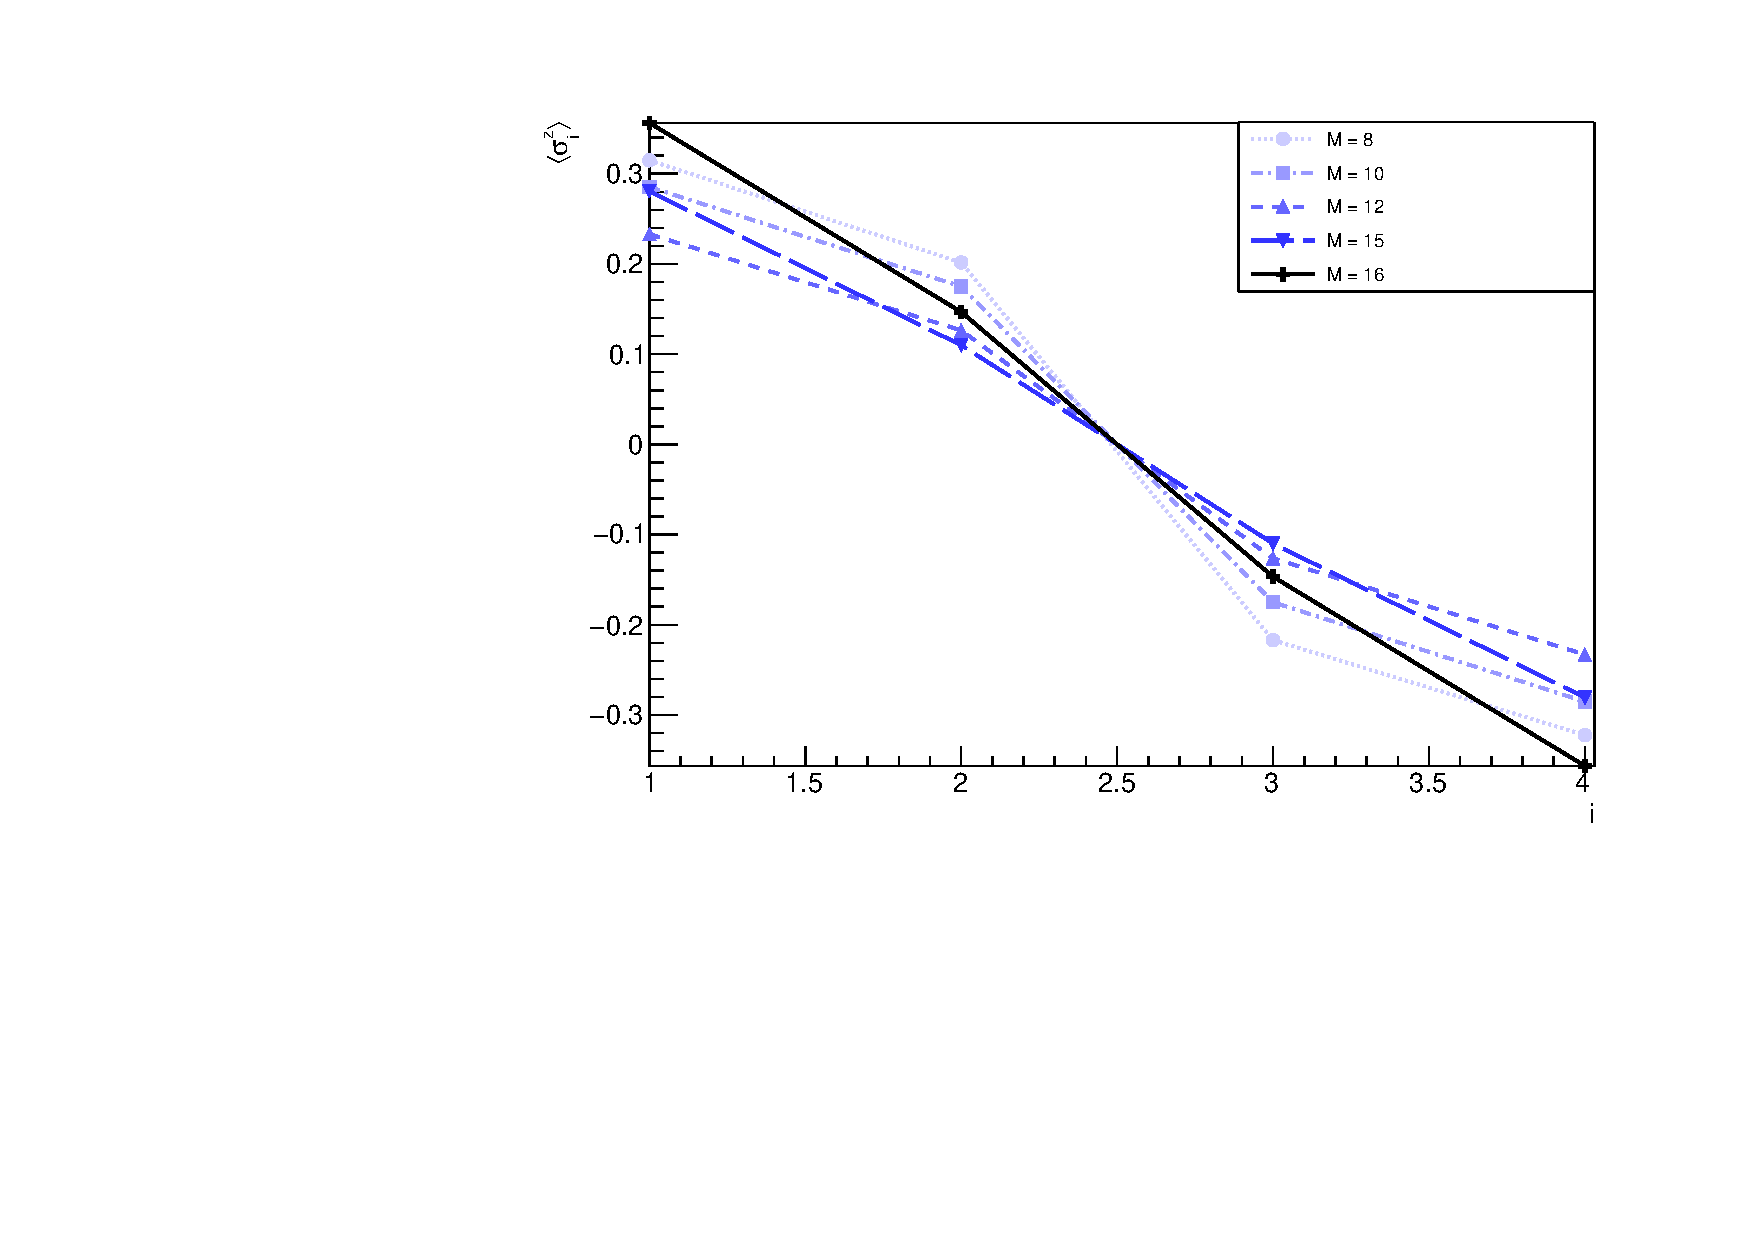
\includegraphics[scale=0.7]{Figures/4sites/4sites_LM_convergenceIncreasingM.pdf}
    \caption{Spin profile of a 4-sites chain for the model described above with $J_z=1$ for several values of corner-space dimensions $M \times M$. The cyan markers are those representing the expectation value of the magnetization calculated by means of a complete set of states of Hilbert space (which has dimension $2^4$).}
    \label{fig:4sites_LM_convergenceIncreasingM}
\end{figure}

As shown in figure~\ref{fig:4sites_LM_convergenceIncreasingM}, it is clear that for such a system the convergence has not been reached. Even for $M = 15$, that covers almost the total Hilbert space dimension, the results are not the convergent ones.

On the other hand, if we consider a model in which every site is coupled to a dissipator, we can see how the magnetization profile gets to convergence starting from $M = 9$ already.


\begin{figure}[H]
    \centering
    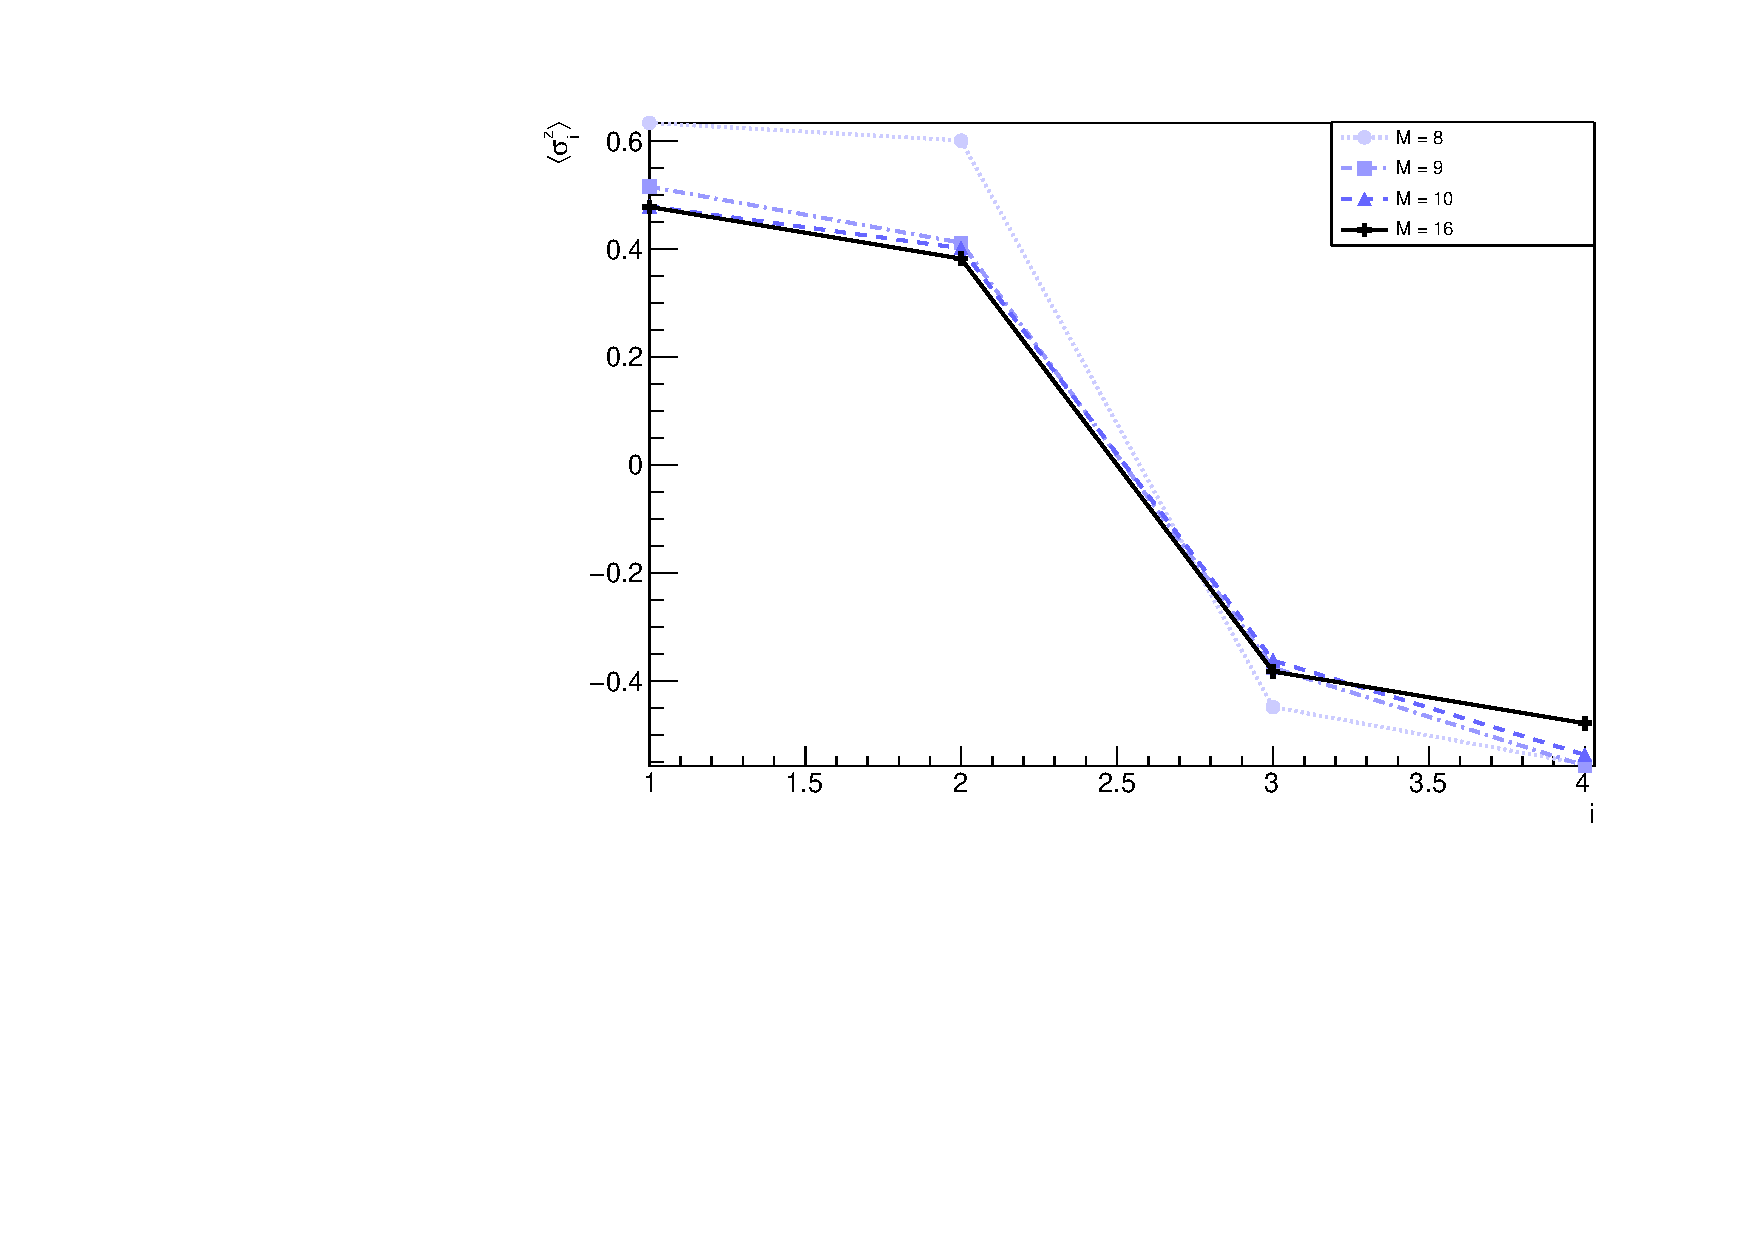
\includegraphics[scale=0.7]{Figures/4sites/4sites_totalDissipators.pdf}
    \caption{Spin profile of a 4-sites chain in which every spin of the chain is coupled to a dissipator. In this case, the convergence is reached for $M<\text{dim}(\mathcal{H})$.}
    \label{fig:4sites_totalDissipators}
\end{figure}

In order to confirm the limitations of this method, the same comparison is done for a longer chain, made up by 8 sites. In this case, the results of CSR method are compared to those of MPO method, since a brute-force diagonalization of the Liouvillian operator would not be possible: it would require a huge amount of memory. We have reason to believe that the results obtained from MPO method are plausible, as we will see in the next sections.

\begin{figure}[H]
    \centering
    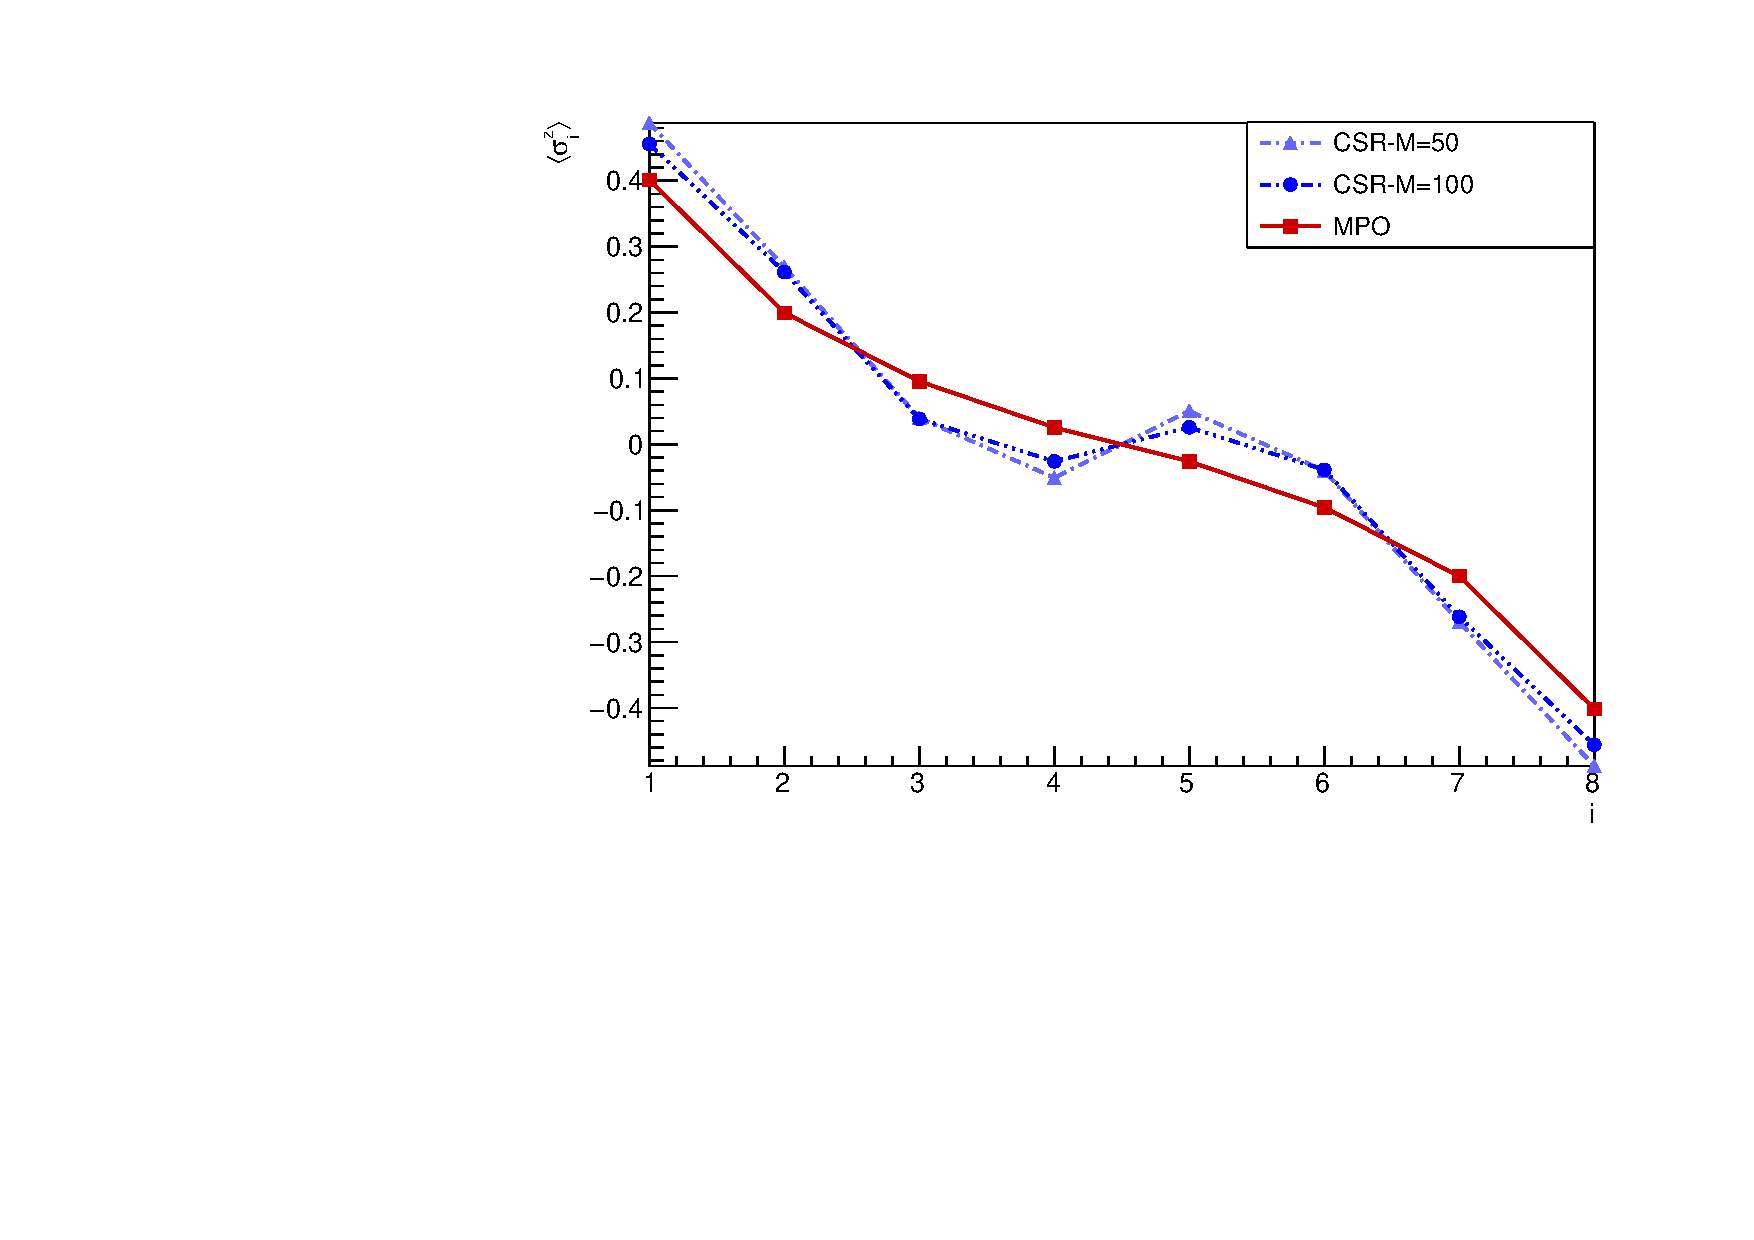
\includegraphics[scale=0.7]{Figures/8sites/1U1D_comparisonCSR_MPO_8site.pdf}
    \caption{Spin profile of a 8-sites chain for the model described in sec.\ref{sec:model}. Significant differences between the data obtained for $M=50$ and $M=100$ are not noticed.}
    \label{fig:1U1D_comparisonCSR_MPO_8site}
\end{figure}

\begin{figure}[H]
    \centering
    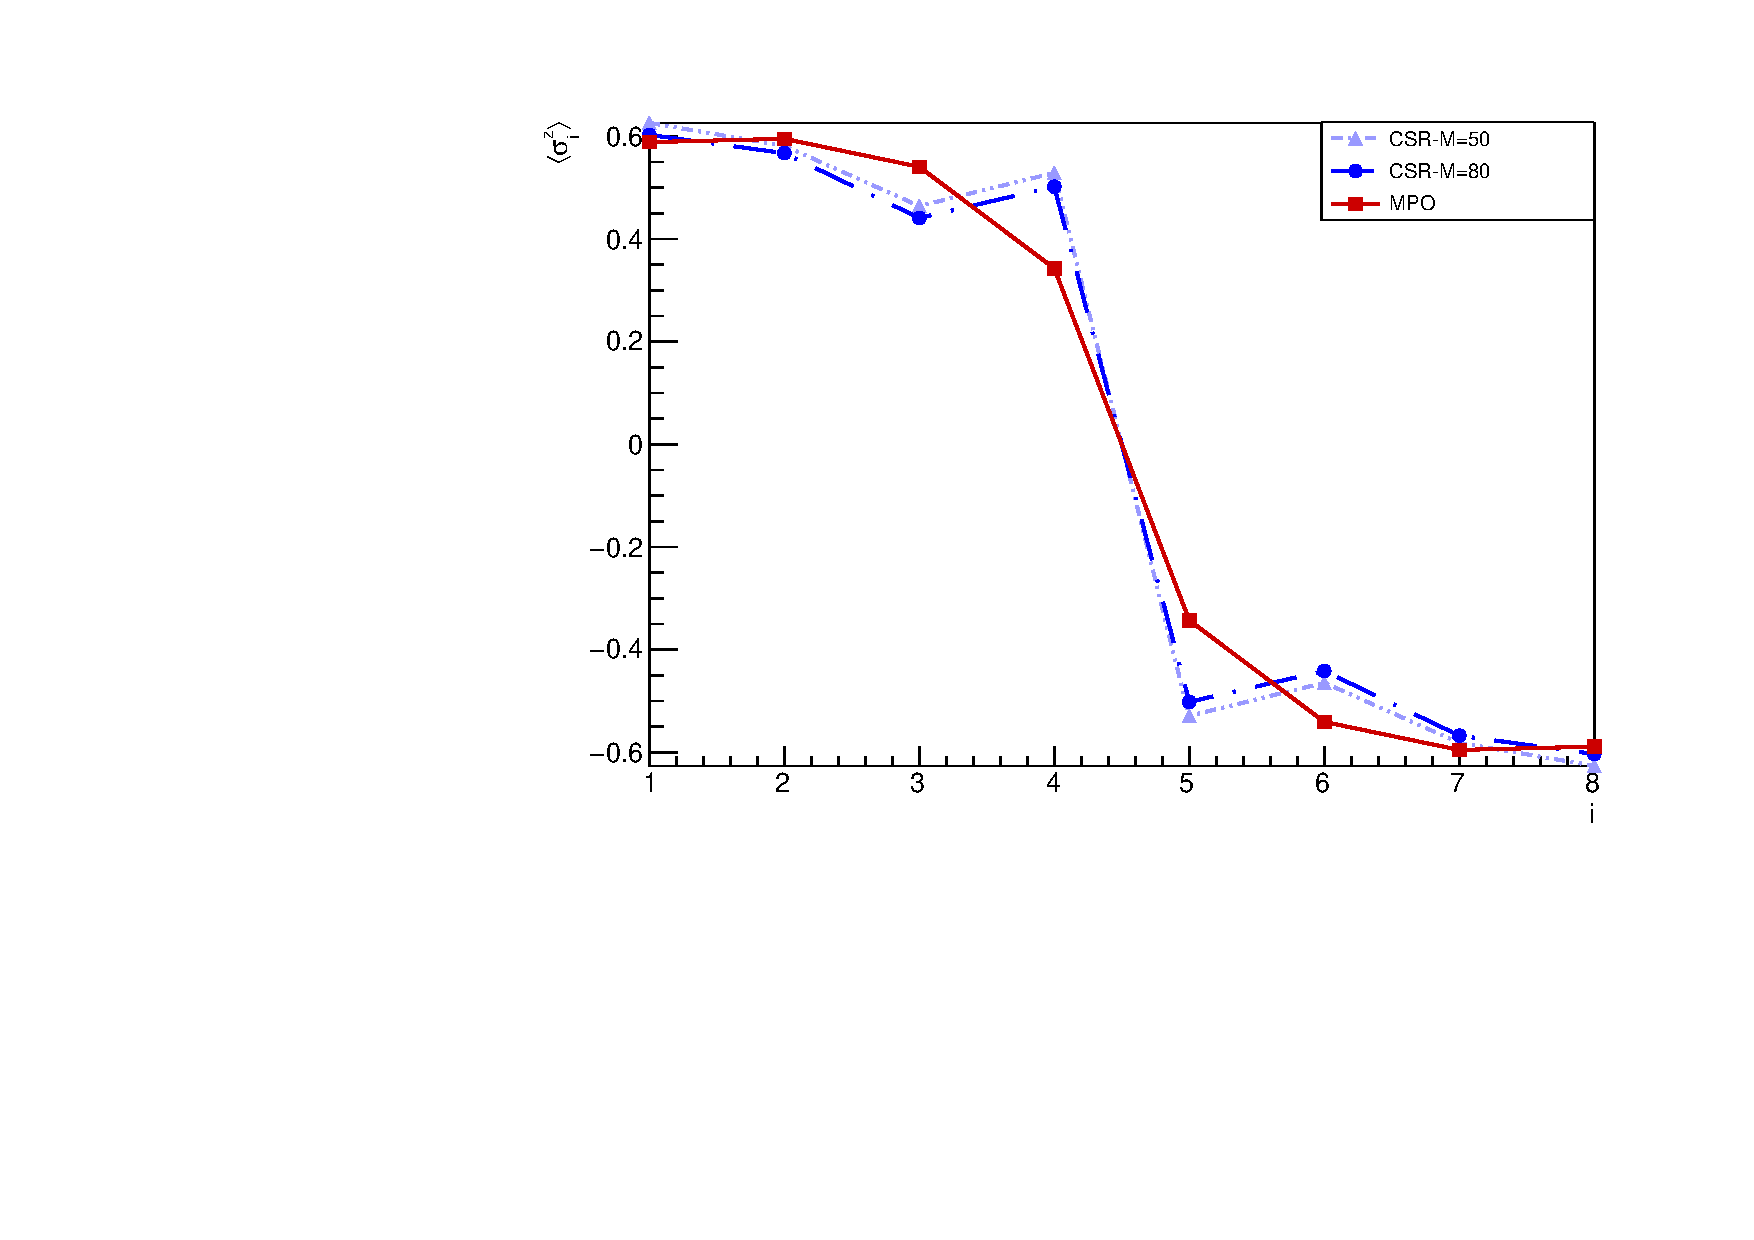
\includegraphics[scale=0.7]{Figures/8sites/8sites_MPOvsCORNER_4U4D.pdf}
    \caption{Spin profile of a 8-sites chain in which every spin of the chain is coupled to a dissipator.}
    \label{fig:8sites_MPOvsCORNER_4U4D}
\end{figure}

In conclusion, in fig.~\ref{fig:LMComparison16s1051} it is displayed the magnetization profile of a 16-sites chain obtained by CSR and MPO methods. It is clear that 

\begin{figure}[H]
    \centering
    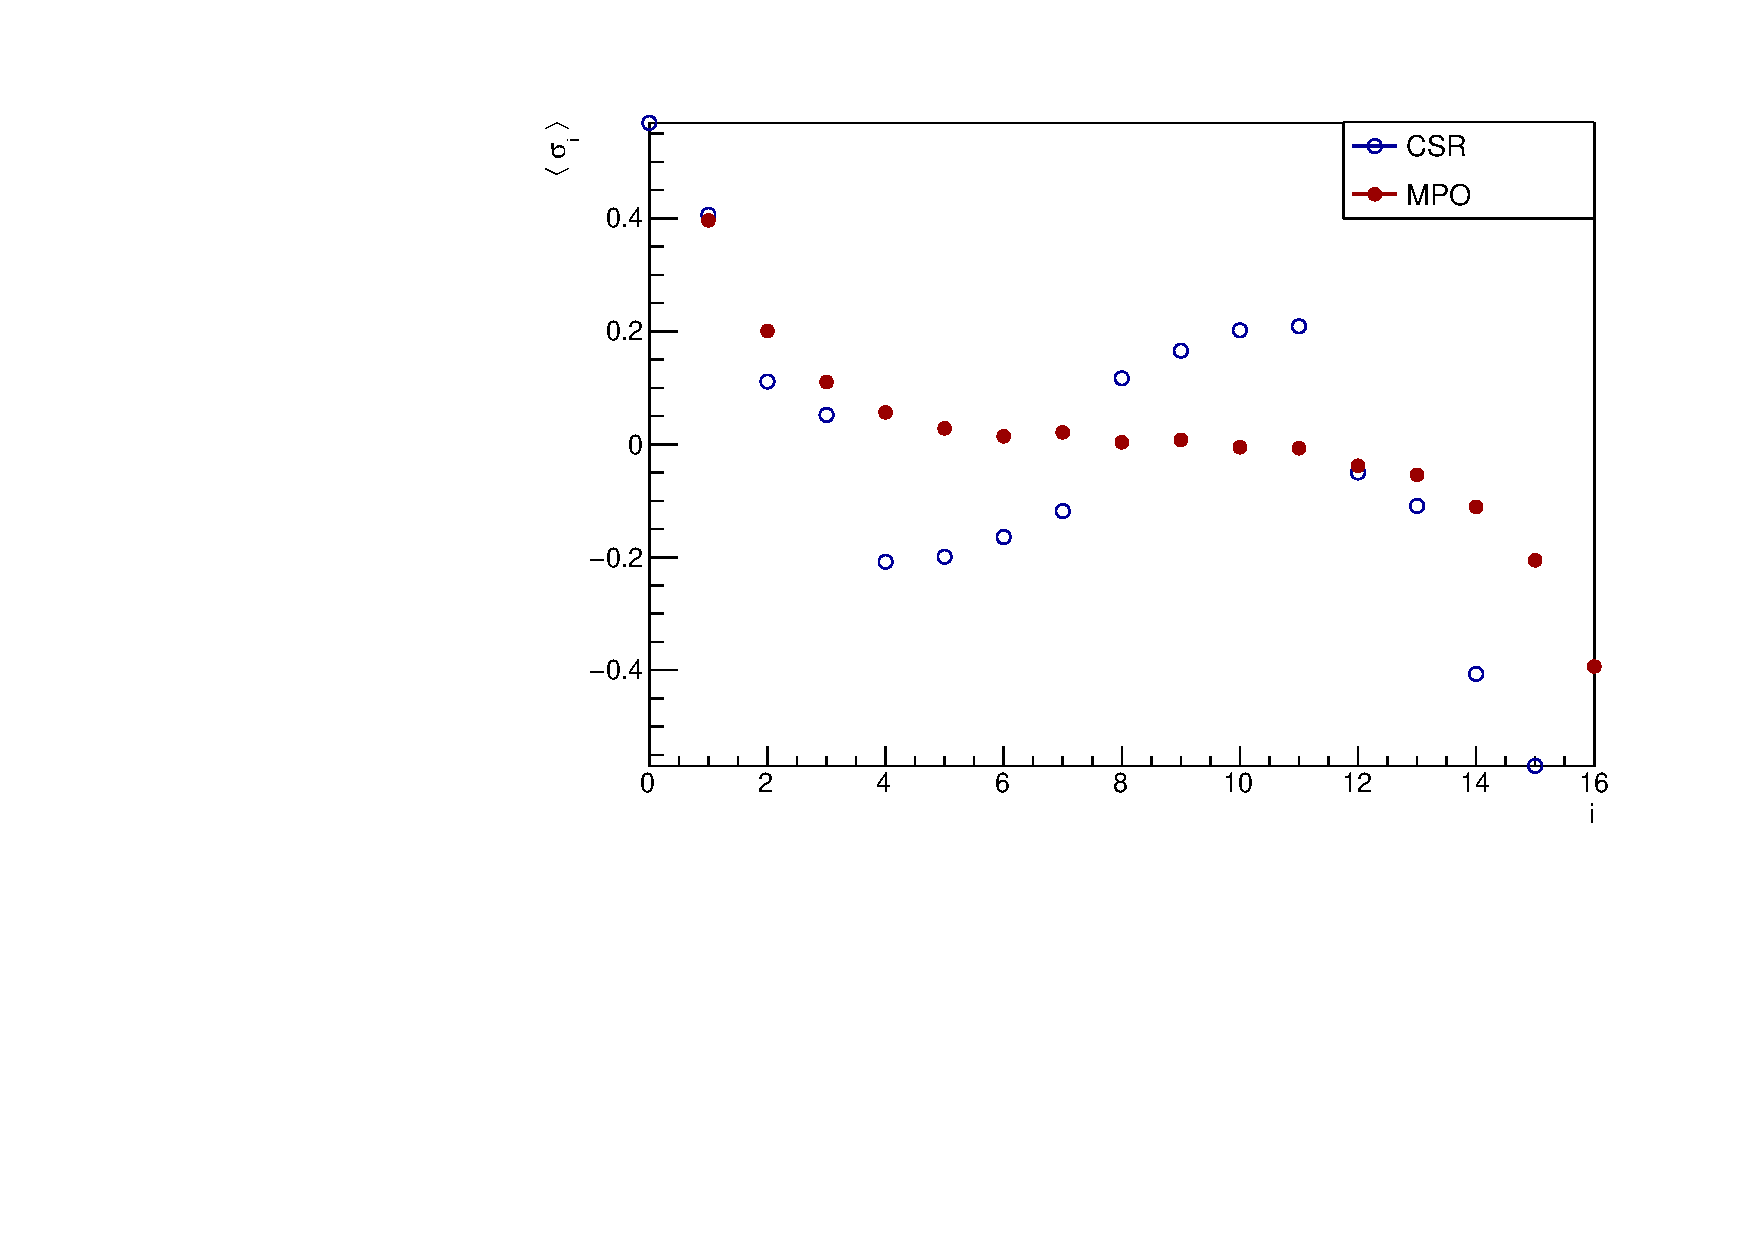
\includegraphics[scale=0.7]{Figures/16sites/LMComparison16s1051.pdf}
    \caption{Spin profile for a 16-sites chain for the model described in section~\ref{sec:model}. Data in red are obtained from MPO method, with m = 80 and T = 2000 and data in blue are obtained from CSR method, with M = 65. It is self-evident the inadequacy of the corner-space size: the complete Hilbert space for such a system has a dimension of $2^{16} \times 2^{16}$.}
    \label{fig:LMComparison16s1051}
\end{figure}



%%%%%%%%%%%%%%%%%%%%%%%%%%%%%%%%%%%%%%%%%%%%%%%%%%%%%%%%%%%%%%%%%%
%%%%%%%%%%%%%%%%%%%%%%%%%%%%%%%%%%%%%%%%%%%%%%%%%%%%%%%%%%%%%%%%%%
%%%%%%%%%%%%%%%%%%%%%%%%%%%%%%%%%%%%%%%%%%%%%%%%%%%%%%%%%%%%%%%%%%
\section{Convergence and Errors}
In order to obtain plausible results, one should make sure of using data 

\begin{figure}[H]
    \label{fig:convergence_mpo_8sites}
    \centering
    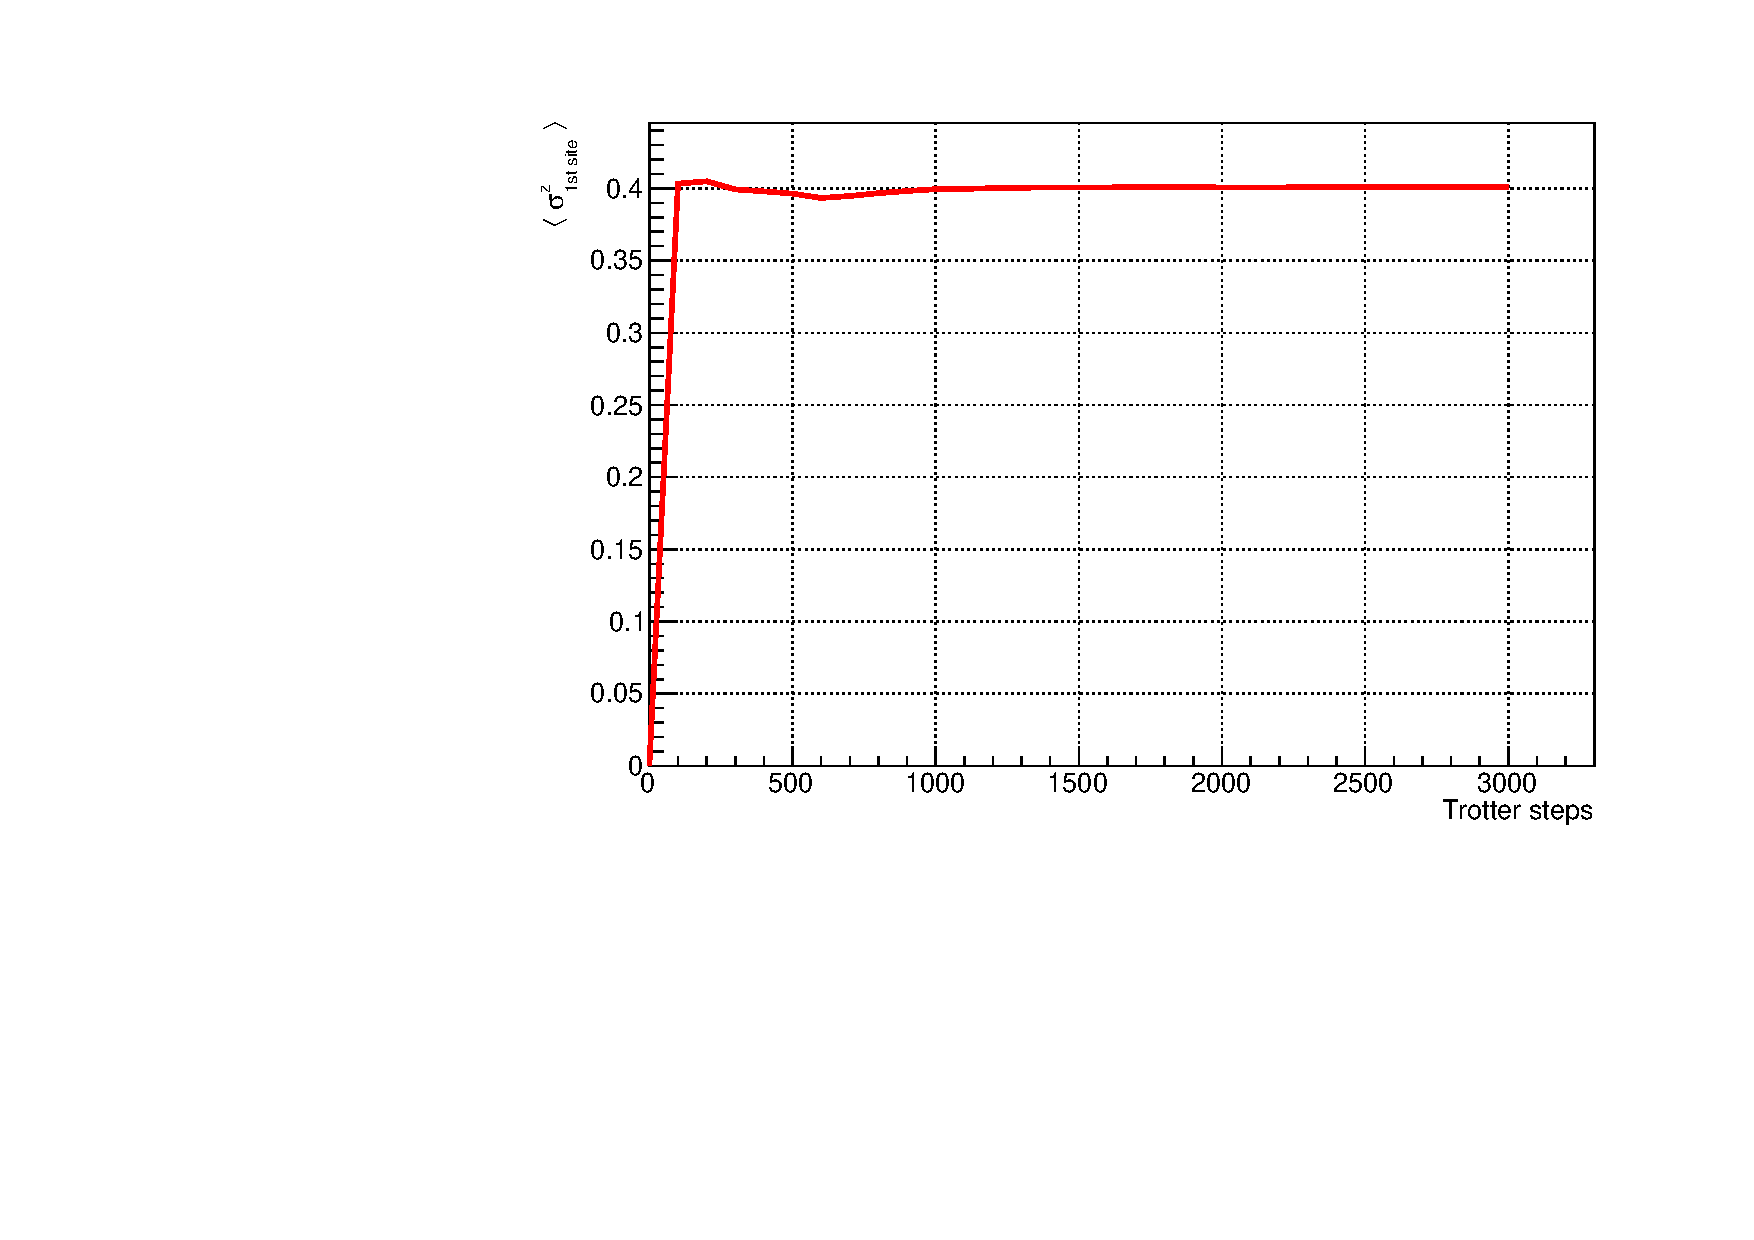
\includegraphics[scale=0.7]{Figures/convergence/Convergence_s8T3000J1051.pdf}
    \caption{Study of convergence of the MPO method for a 8-sites chain, for bond dimension m = 100 and T = 3000.}
    \label{fig:convergenceMPO_8sites}
\end{figure}

\begin{figure}[H]
    \label{fig:convergence_mpo_8sites}
    \centering
    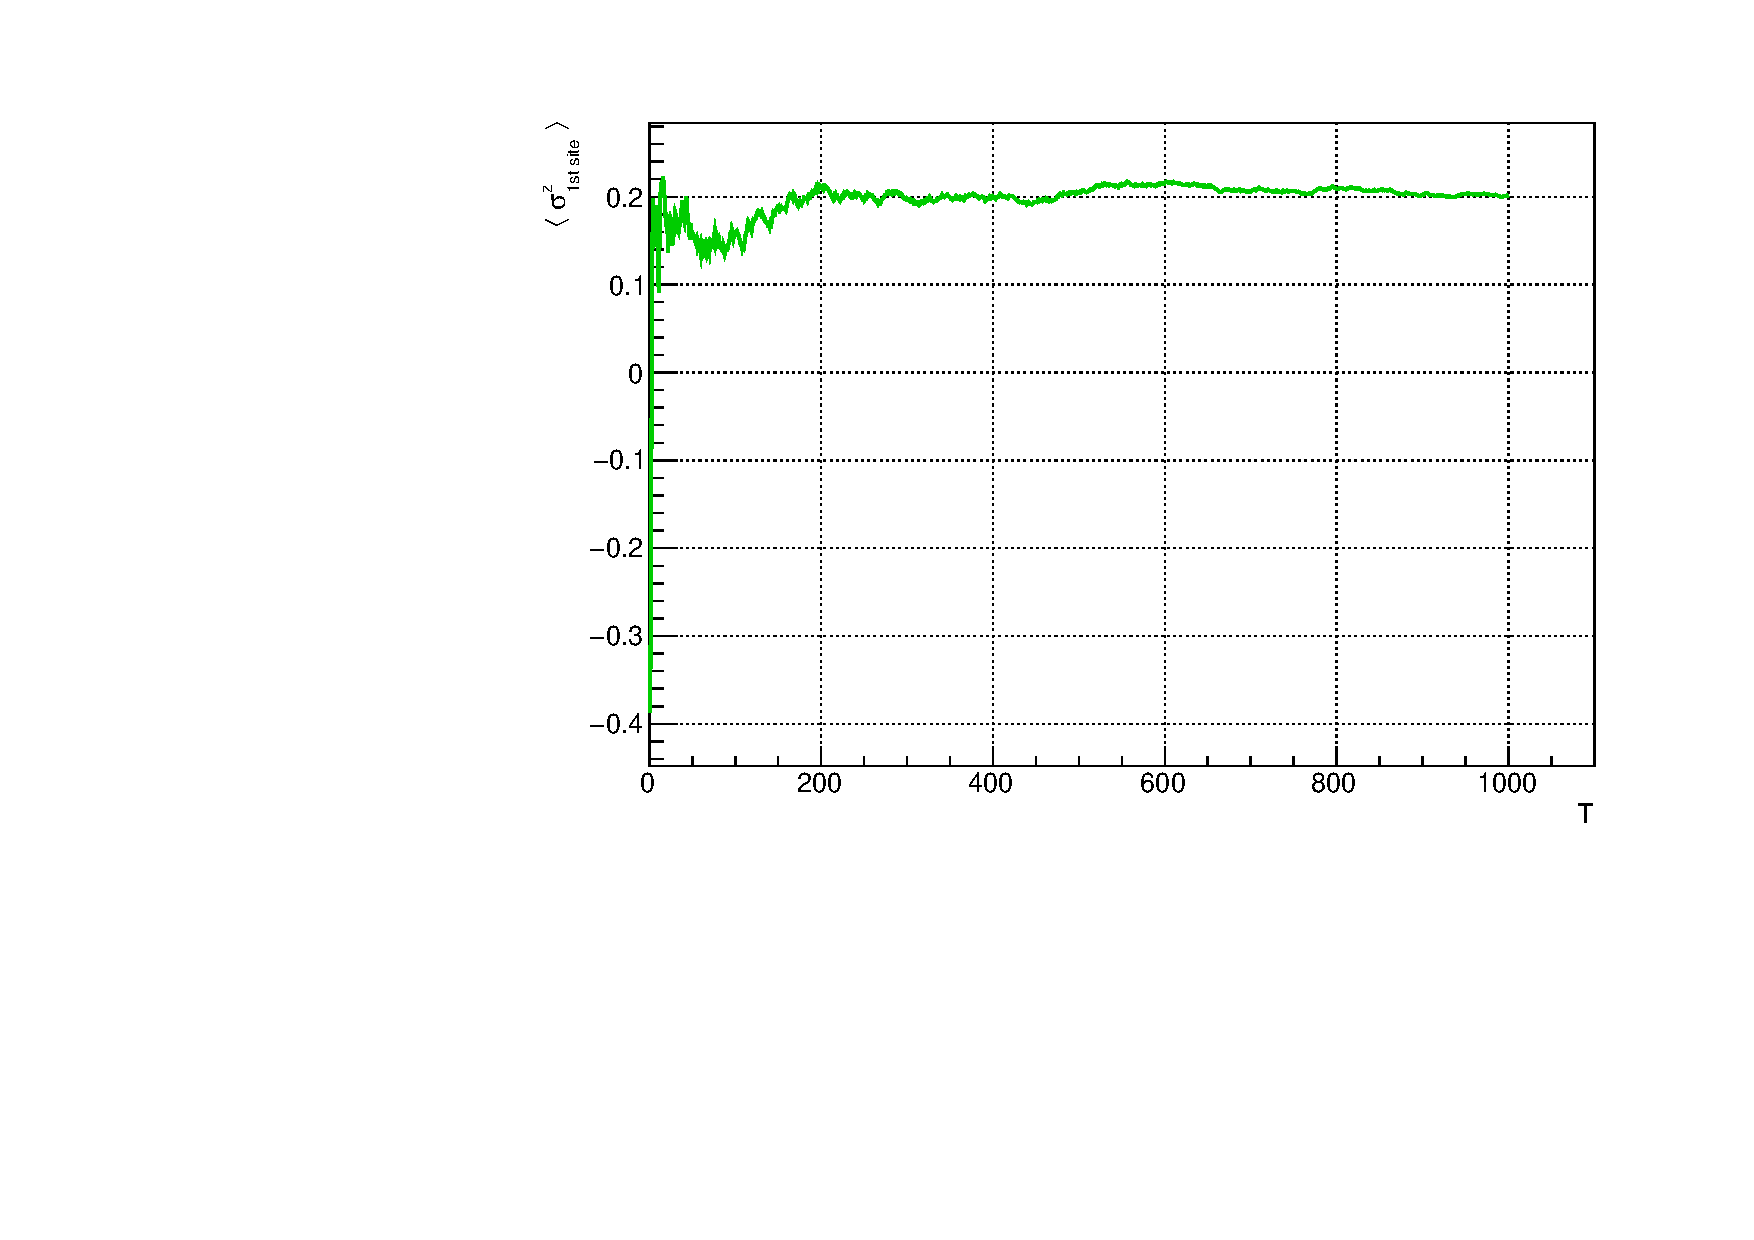
\includegraphics[scale=0.7]{Figures/convergence/Convergence_s8J10505.pdf}
    \caption{Study of convergence of the QT method for a 8-sites chain, for time step $dt=0.1$, T being the whole elapsed time.}
    \label{fig:convergenceMPO_8sites}
\end{figure}

\begin{figure}[H]
    \centering
    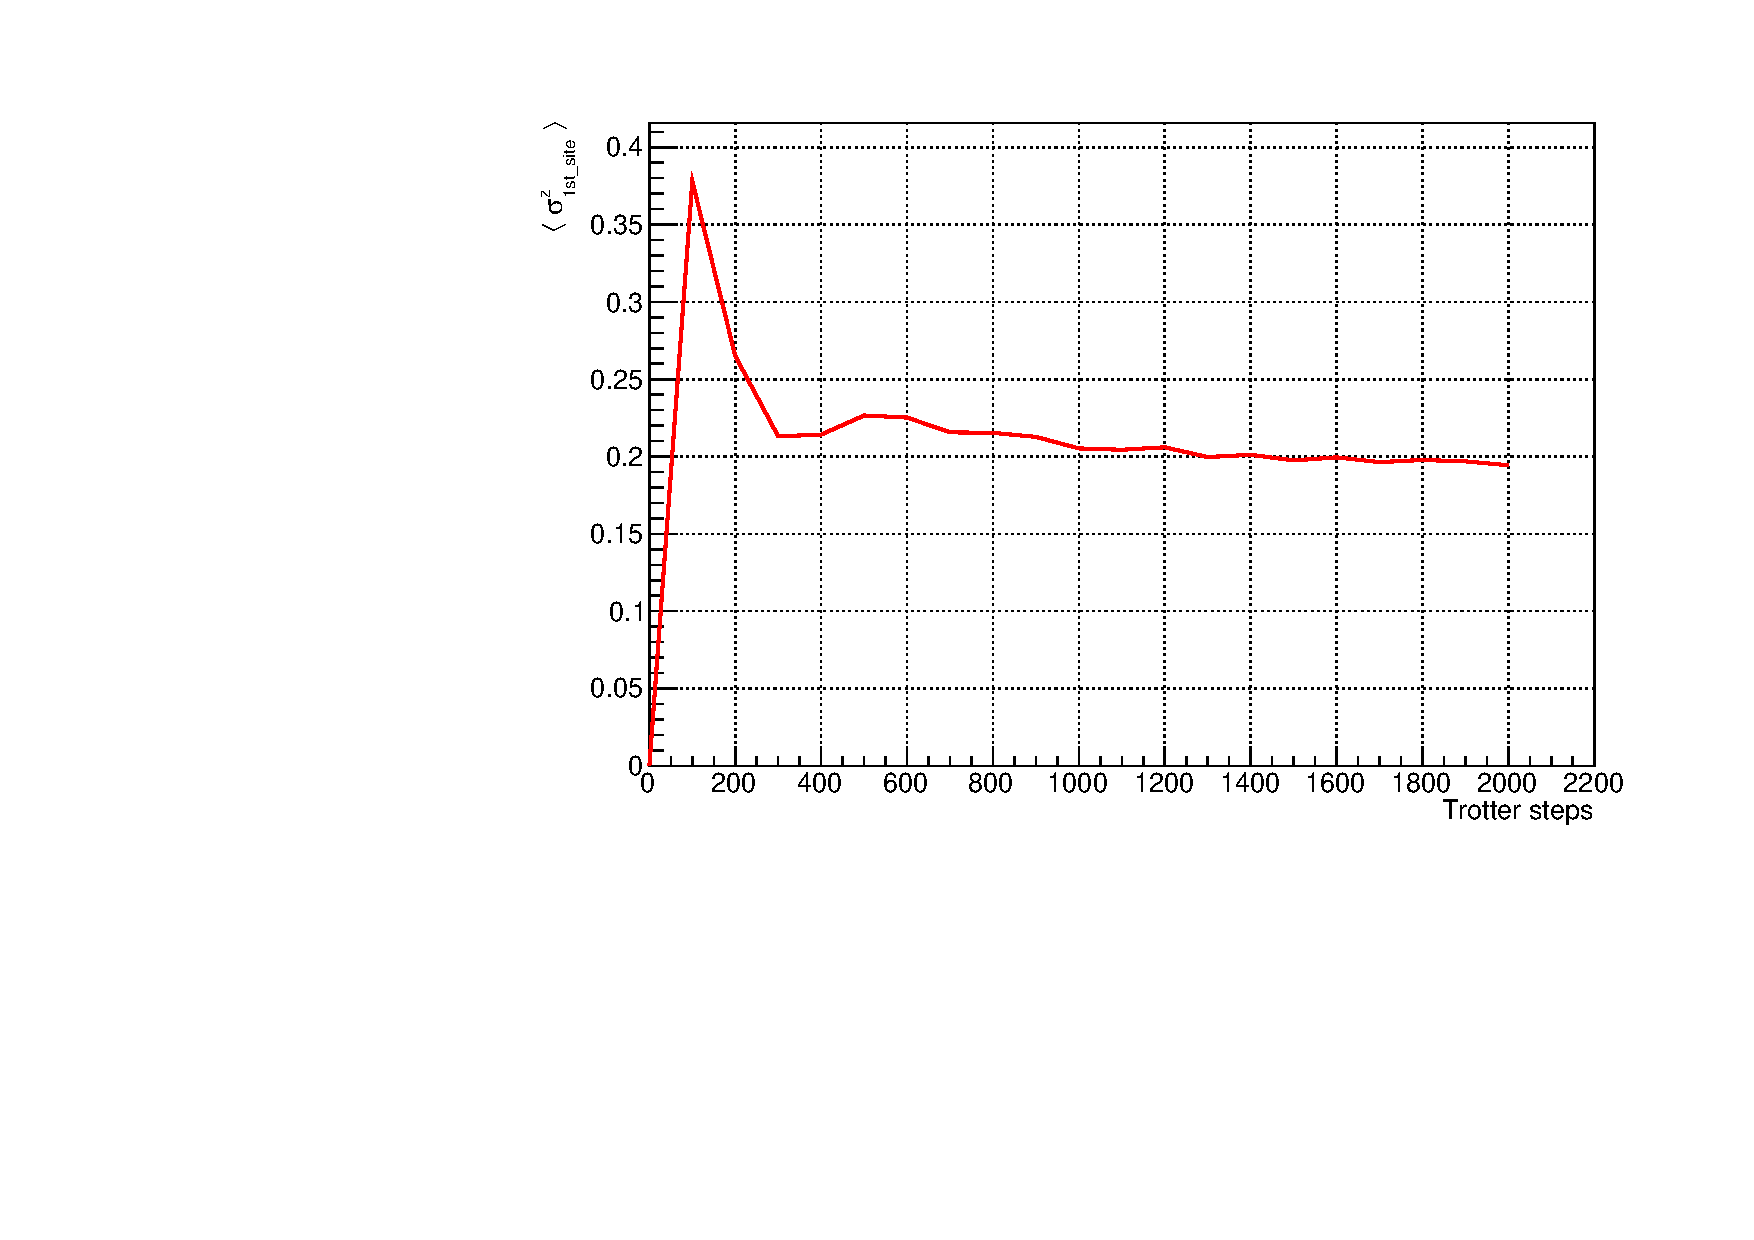
\includegraphics[scale=0.7]{Figures/12sites/ConvergenceLML012m060Time002000_J10505.pdf}
    \caption{Study of convergence of the MPO method for a 12-sites chain, for bond dimension m = 60 and T = 2000.}
    \label{fig:my_label}
\end{figure}

\textcolor{red}{NUMERICAL ERRORS?}

%%%%%%%%%%%%%%%%%%%%%%%%%%%%%%%%%%%%%%%%%%%%%%%%%%%%%%%%%%%%%%%%%%
%%%%%%%%%%%%%%%%%%%%%%%%%%%%%%%%%%%%%%%%%%%%%%%%%%%%%%%%%%%%%%%%%%
%%%%%%%%%%%%%%%%%%%%%%%%%%%%%%%%%%%%%%%%%%%%%%%%%%%%%%%%%%%%%%%%%%
\section{Magnetization Profile}
\label{sec:magn_profile}
The first observable examined is the magnetization of the chain, i.e. the expectation value $\langle \sigma^z \rangle$ of the Pauli matrix $\sigma^z$ for each site. 

\subsection{MPO and QT Comparison}
First of all, a comparison between MPO and QT methods can be done for a 8-sites chain. As it can seen in 

\begin{figure}[H]
    \centering
    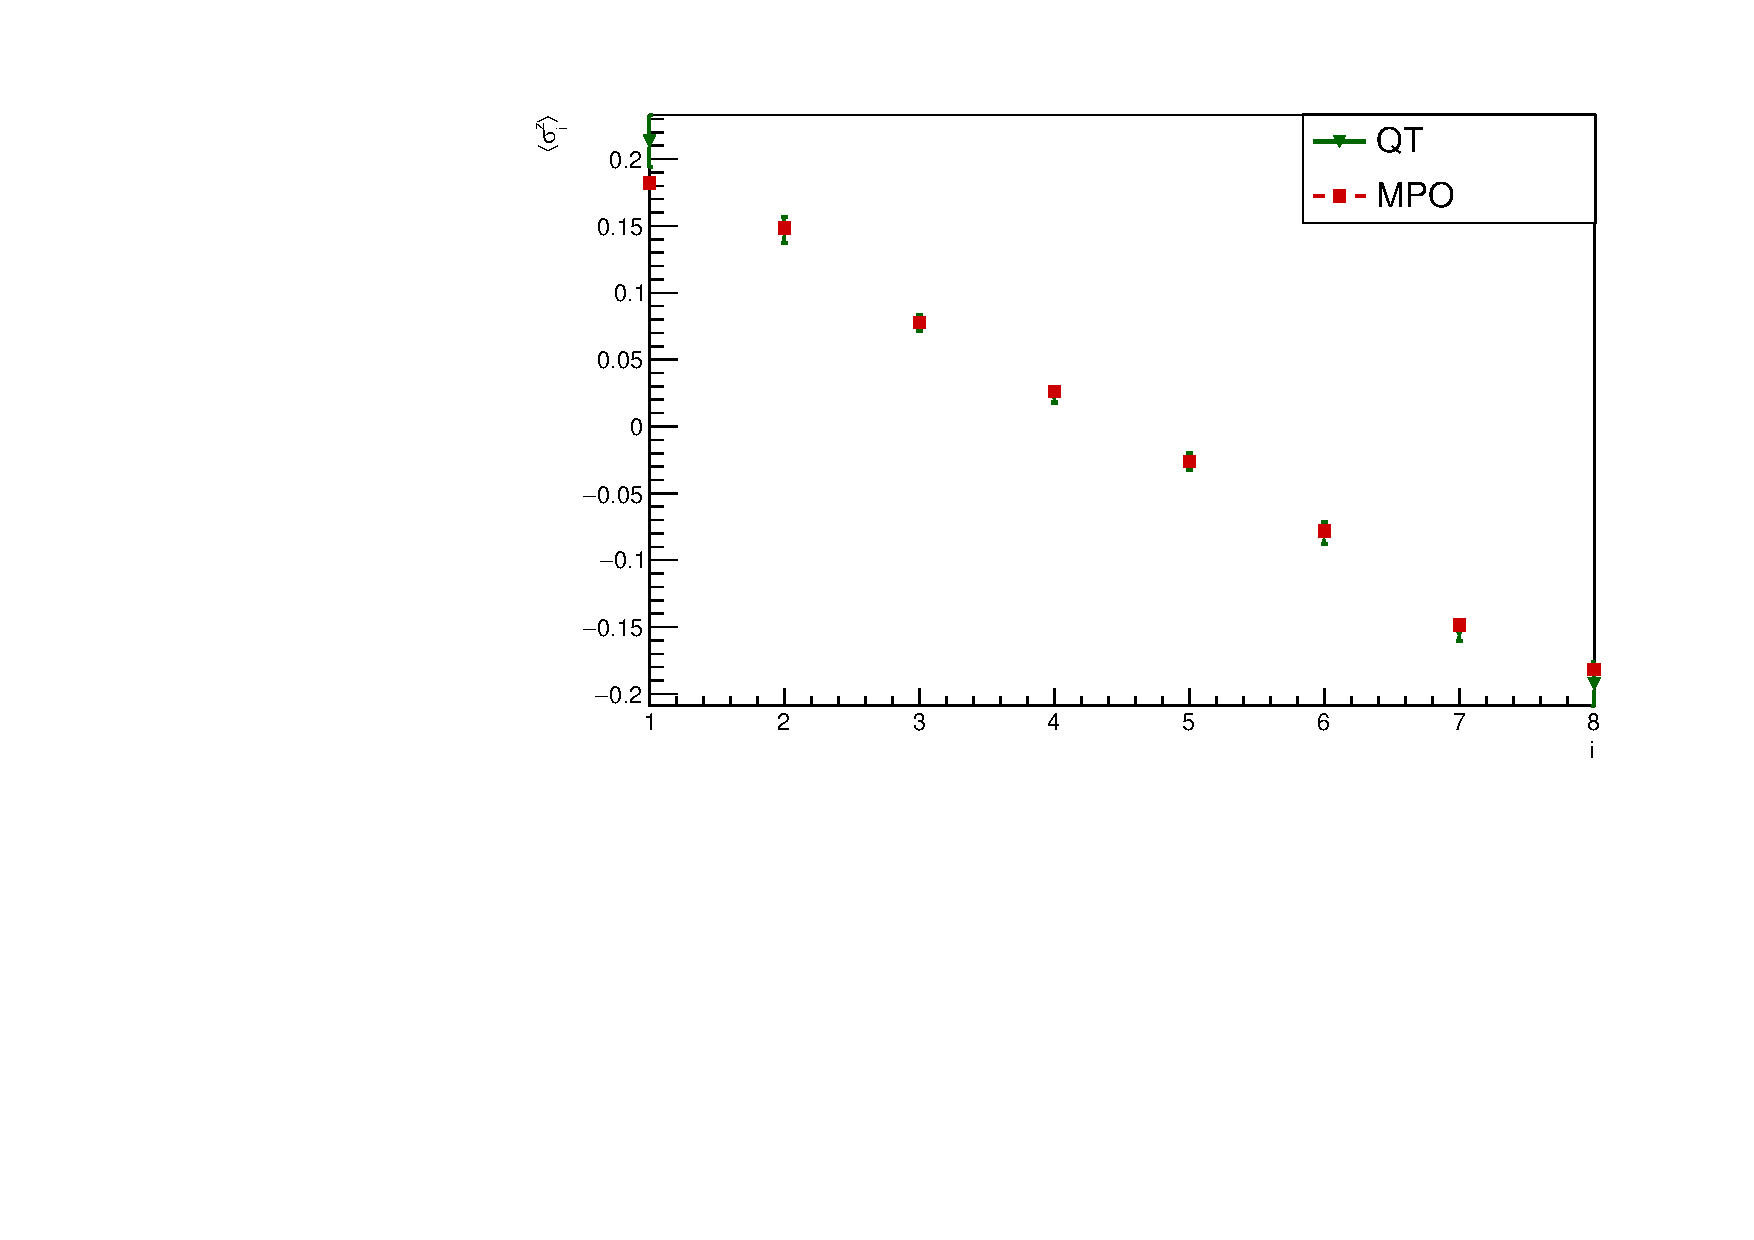
\includegraphics[scale=0.7]{Figures/8sites/LMComparison_8sJ10505.pdf}
    \caption{Spin profile for a 8-sites chain characterized by $\gamma~=~1, J_x=1, J_y=0.5, J_z=0.5$; \emph{i} stands for the site index.}
    \label{fig:8sites_LMcomparisonJz05}
\end{figure}

\begin{figure}[H]
    \centering
    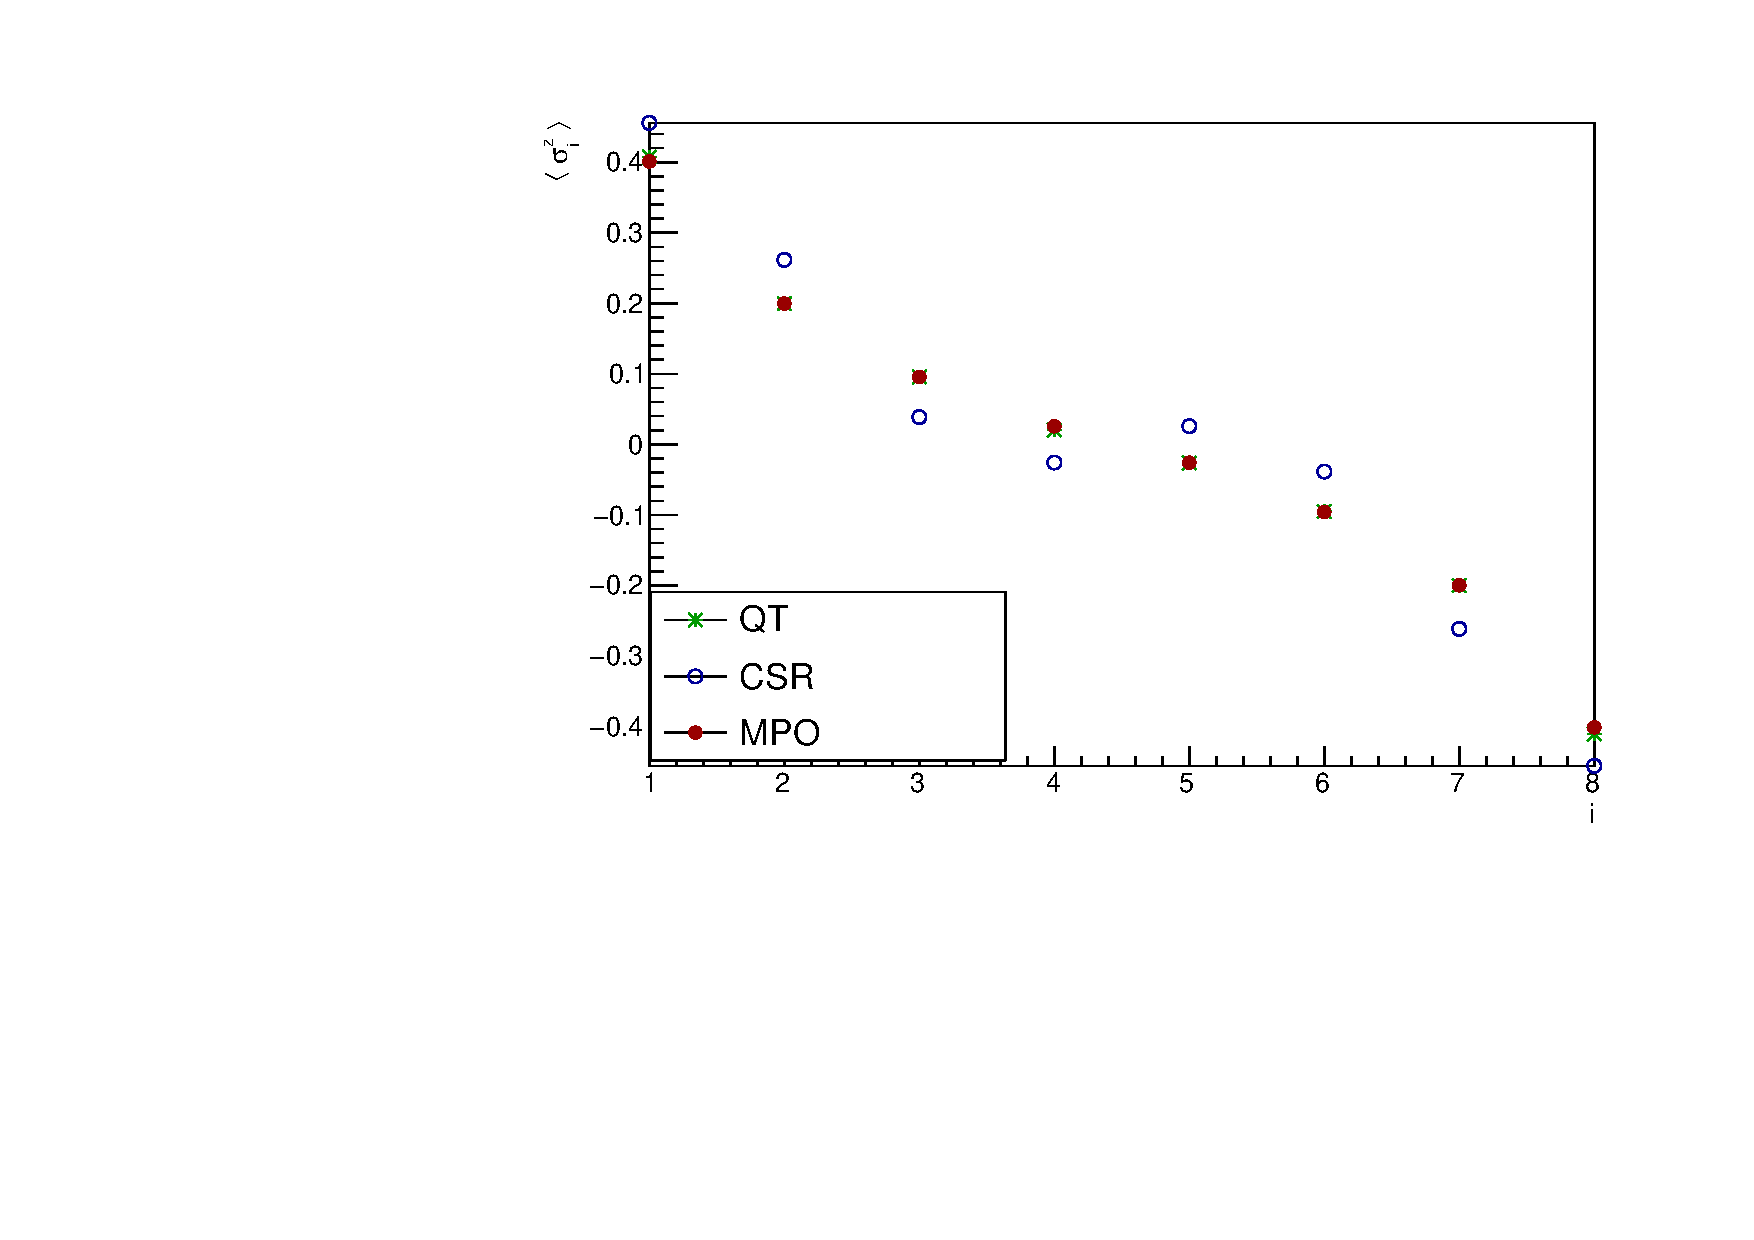
\includegraphics[scale=0.7]{Figures/8sites/LMComparison_8sJ1051.pdf}
    \caption{Spin profile for a 8-sites chain characterized by $\gamma~=~1, J_x=1, J_y=0.5, J_z=1$; \emph{i} stands for the site index.}
    \label{fig:8sites_LMcomparisonJz1}
\end{figure}

\begin{figure}[H]
    \centering
    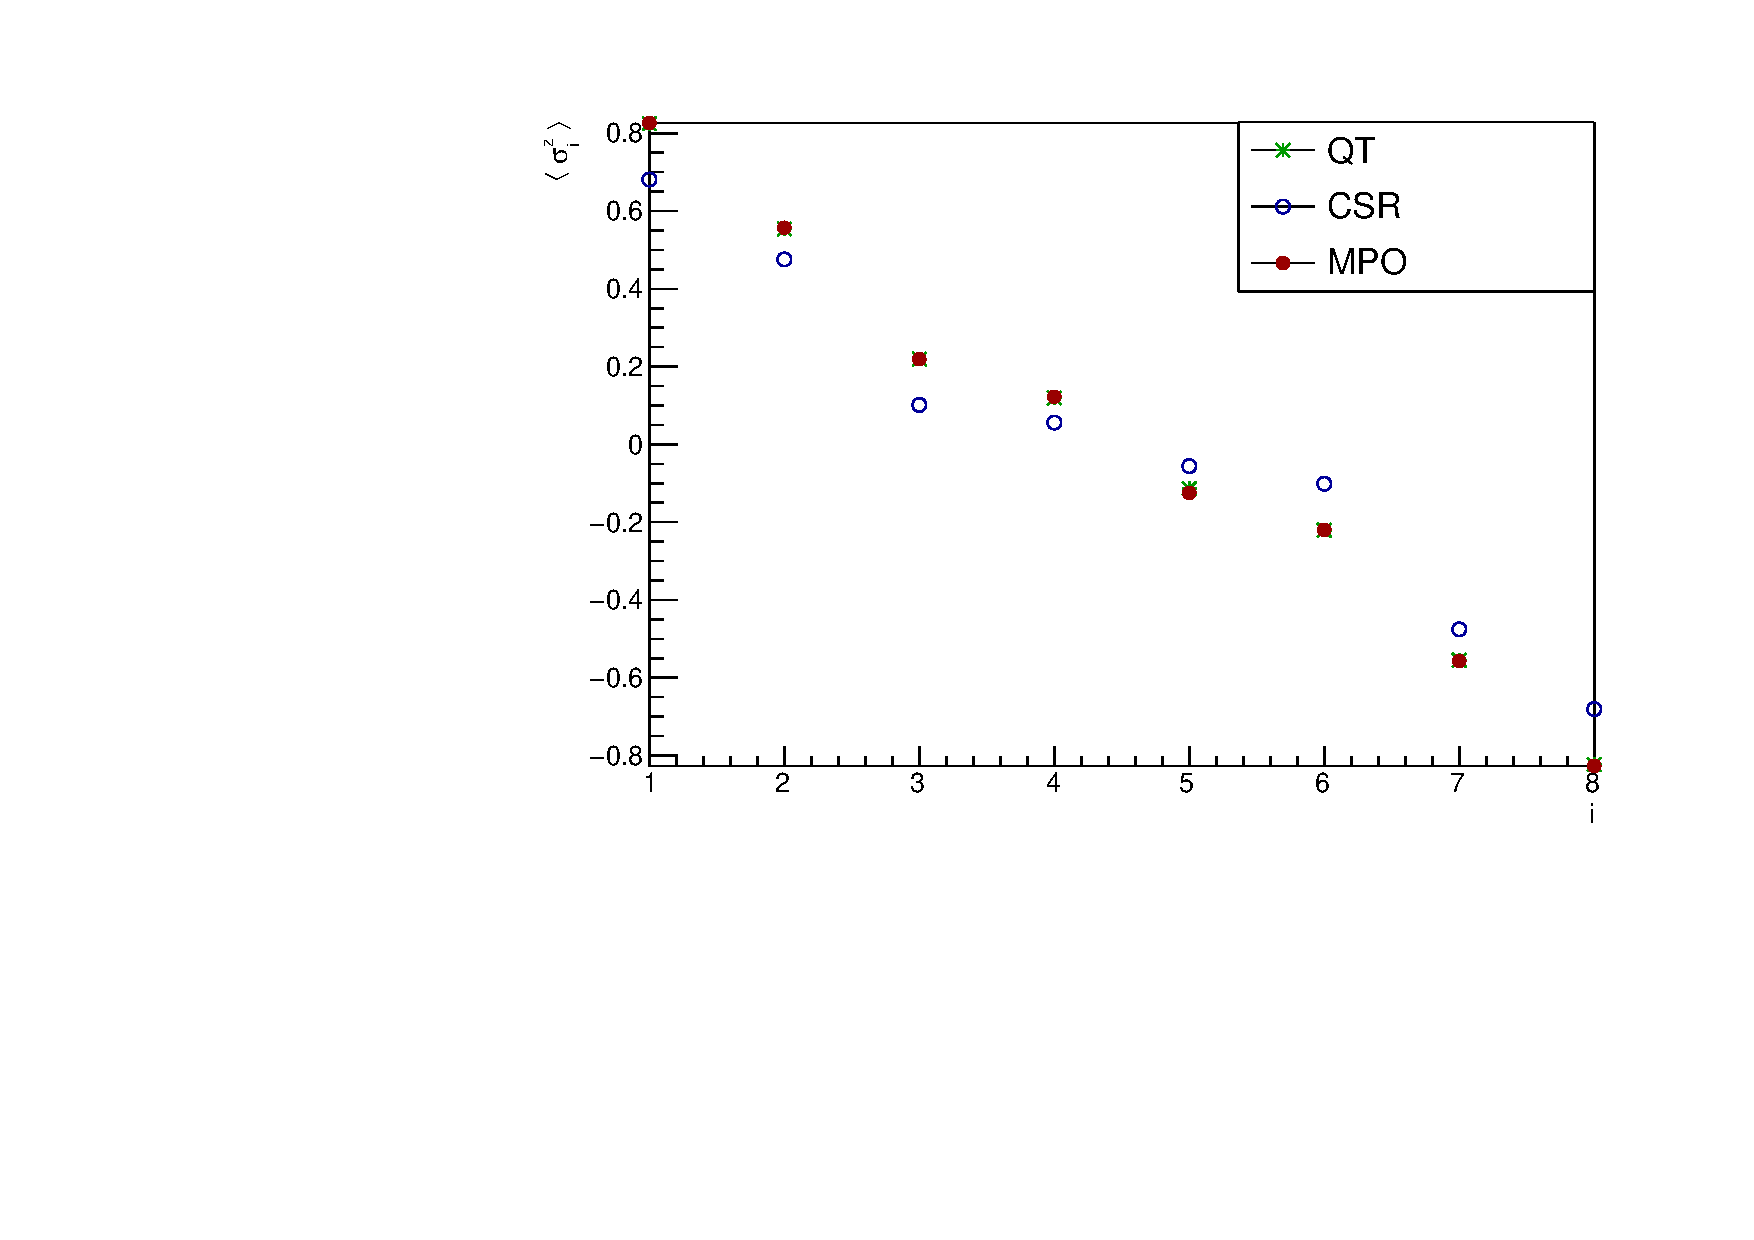
\includegraphics[scale=0.7]{Figures/8sites/LM_8s_J10515.pdf}
    \caption{Spin profile for a 8-sites chain characterized by $\gamma~=~1, J_x=1, J_y=0.5, J_z=1.5$.}
    \label{fig:my_label}
\end{figure}

It can be interesting seeing if the magnetization changes its profile for different chain lengths; now let us see the case of a \textbf{12-sites} chain for different values of $J_z$ as done previously. The following data are obtained from MPO method.

\begin{figure}[H]
    \centering
    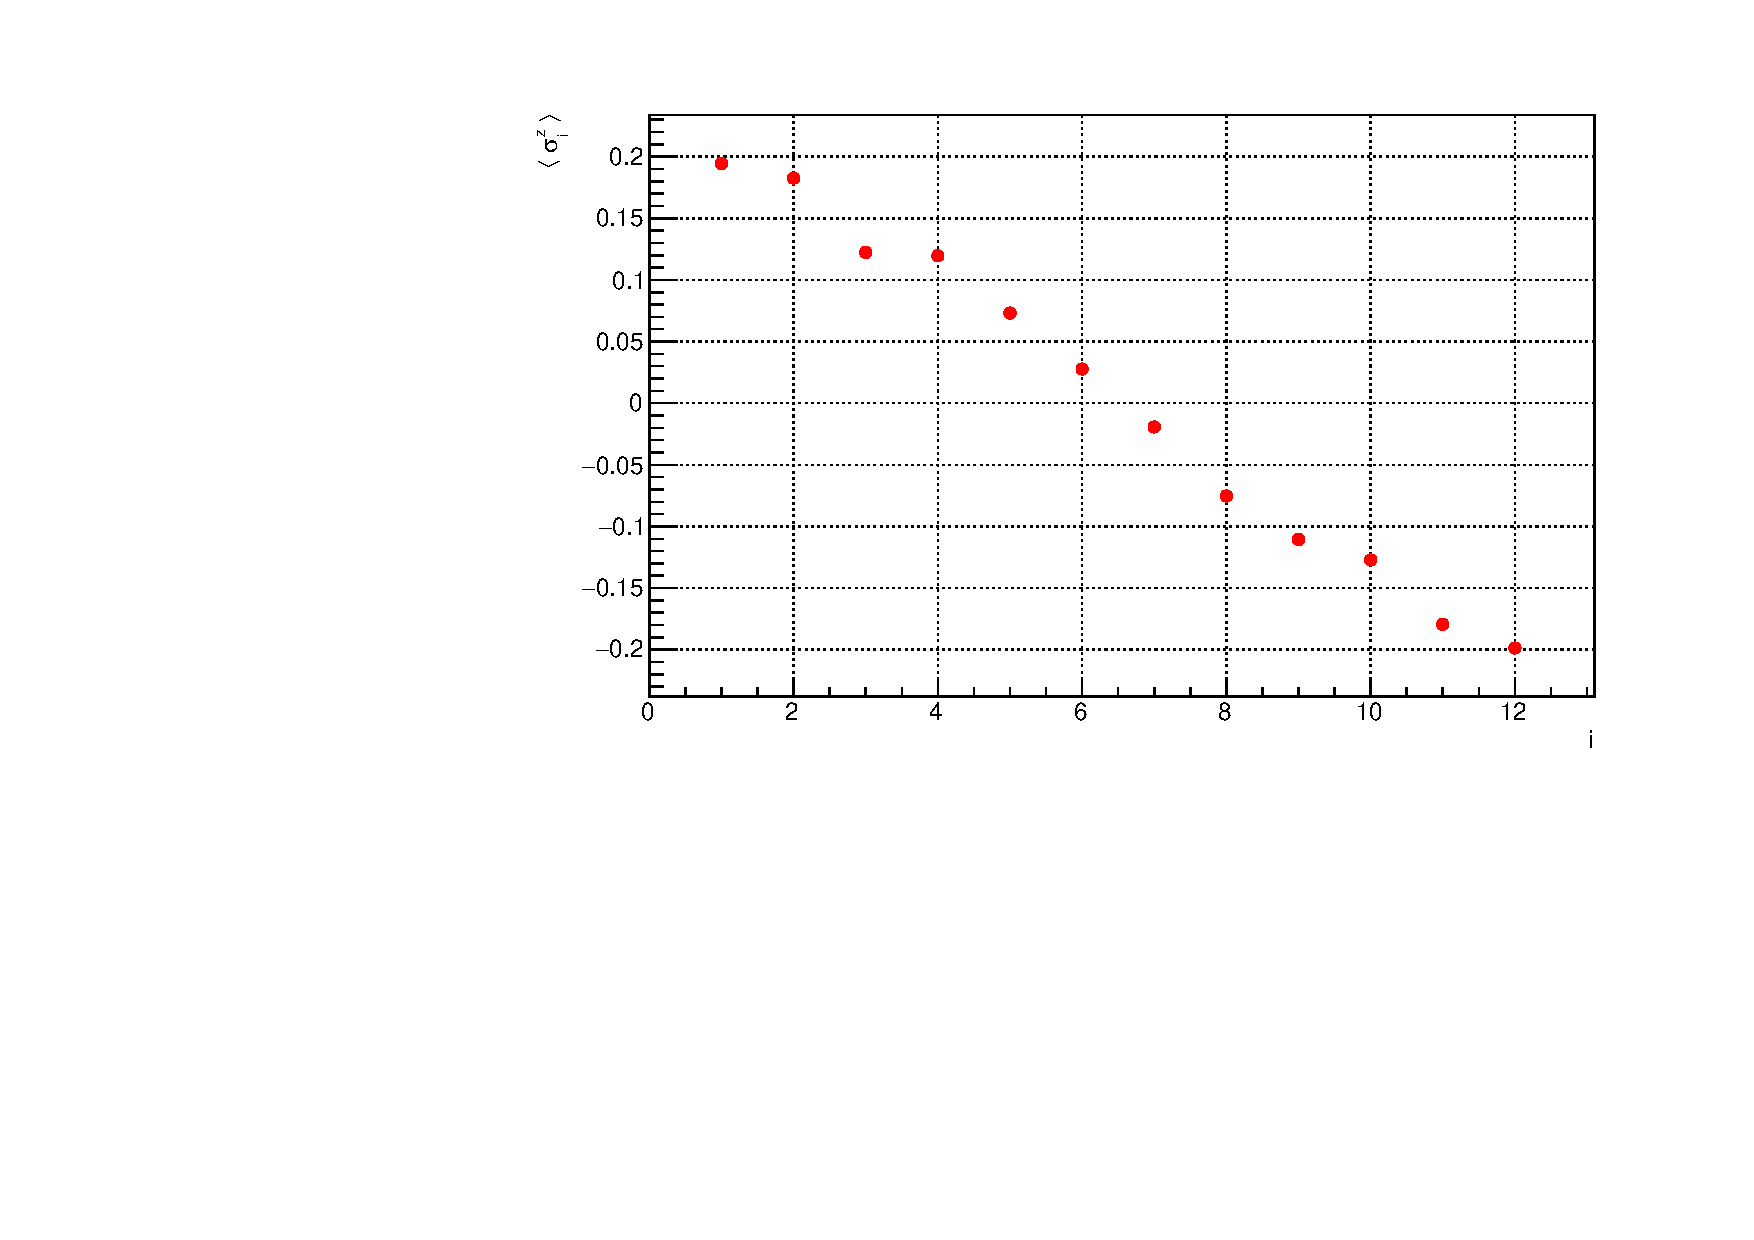
\includegraphics[scale=0.7]{Figures/12sites/LML012m060Time002000_J10505.pdf}
    \caption{Spin profile for a 12-sites chain characterized by $\gamma~=~1, J_x=1, J_y=0.5, J_z=0.5$. Data are obtained from MPO method, with m = 60 and T = 2000.}
    \label{fig:my_label}
\end{figure}

\begin{figure}[H]
    \centering
    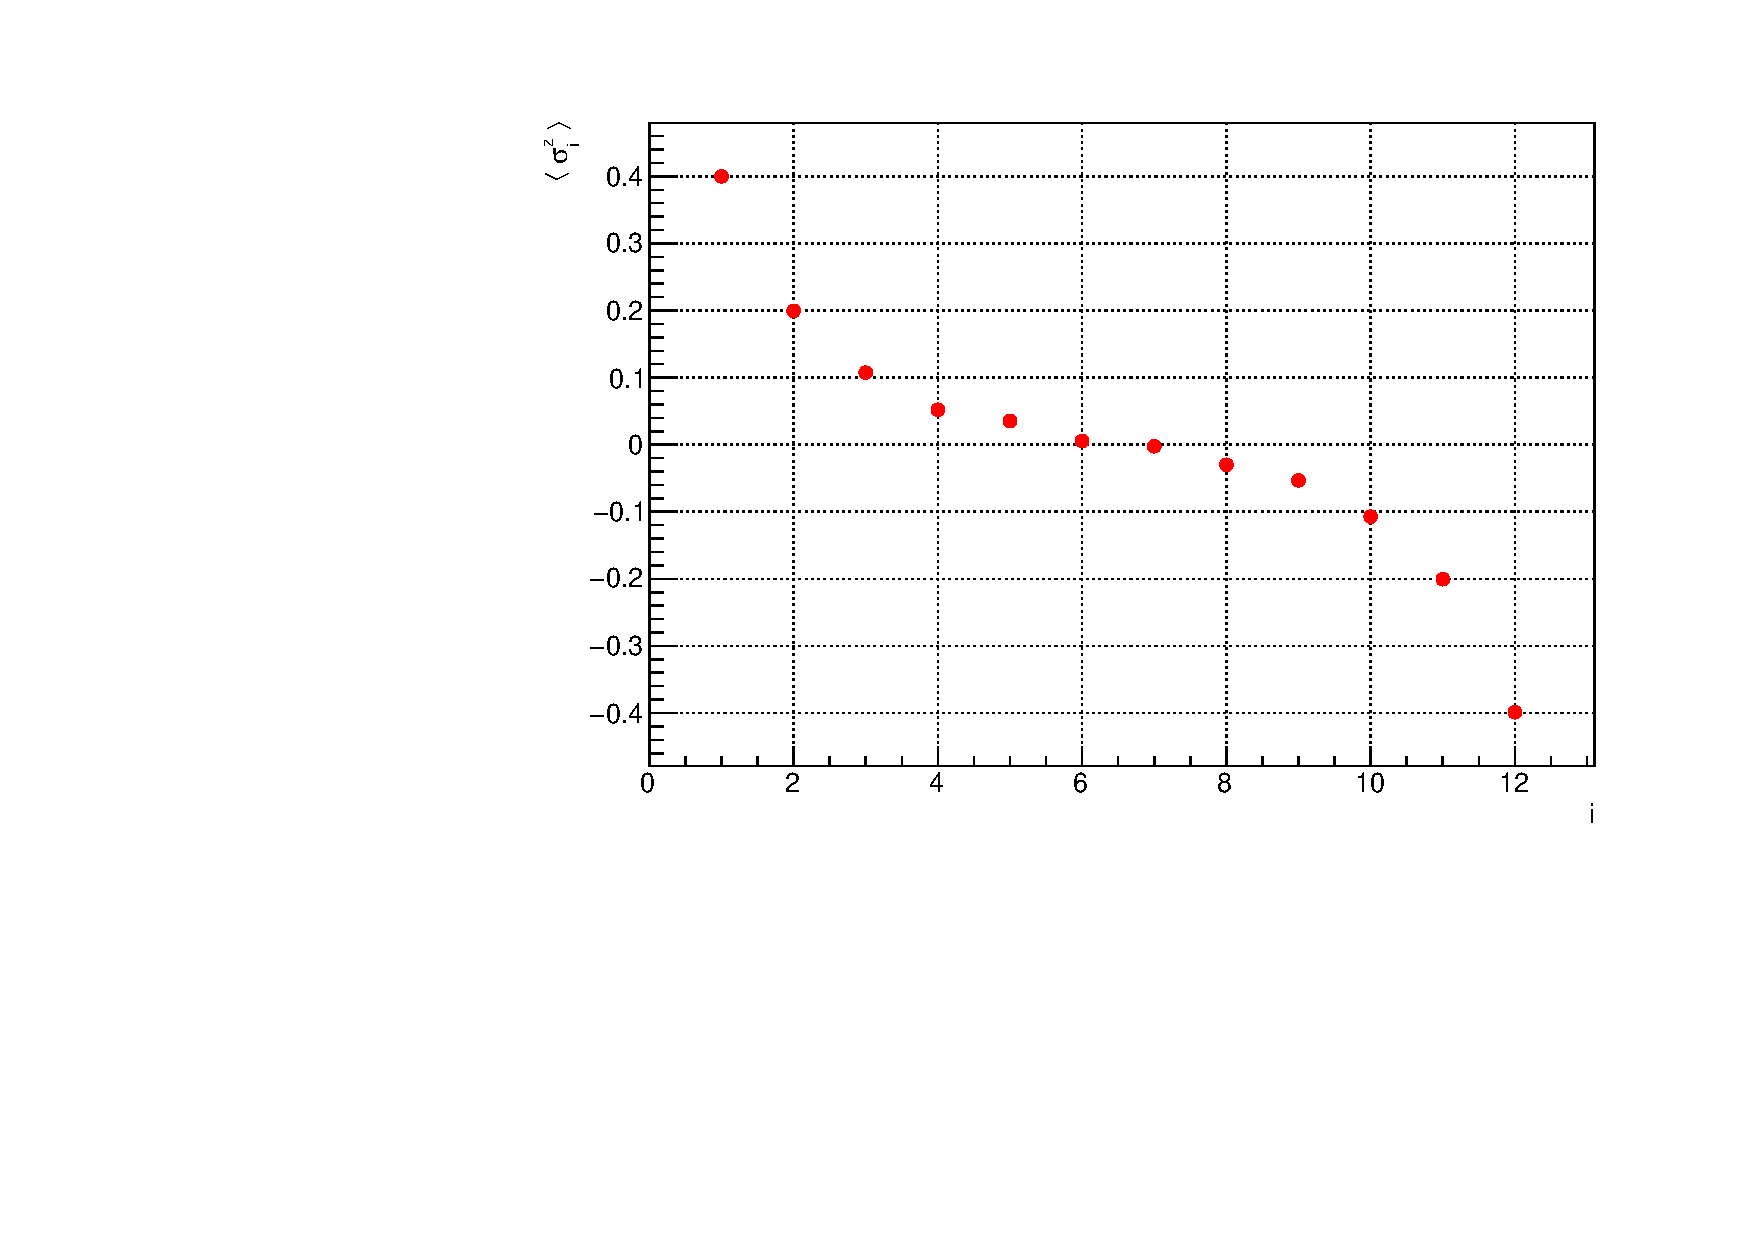
\includegraphics[scale=0.7]{Figures/12sites/LML012m060Time002000_J1051.pdf}
    \caption{Spin profile for a 12-sites chain characterized by $\gamma~=~1, J_x=1, J_y=0.5, J_z=1.$. Data are obtained from MPO method, with m = 60 and T = 2000.}
    \label{fig:my_label}
\end{figure}

\begin{figure}[H]
    \centering
    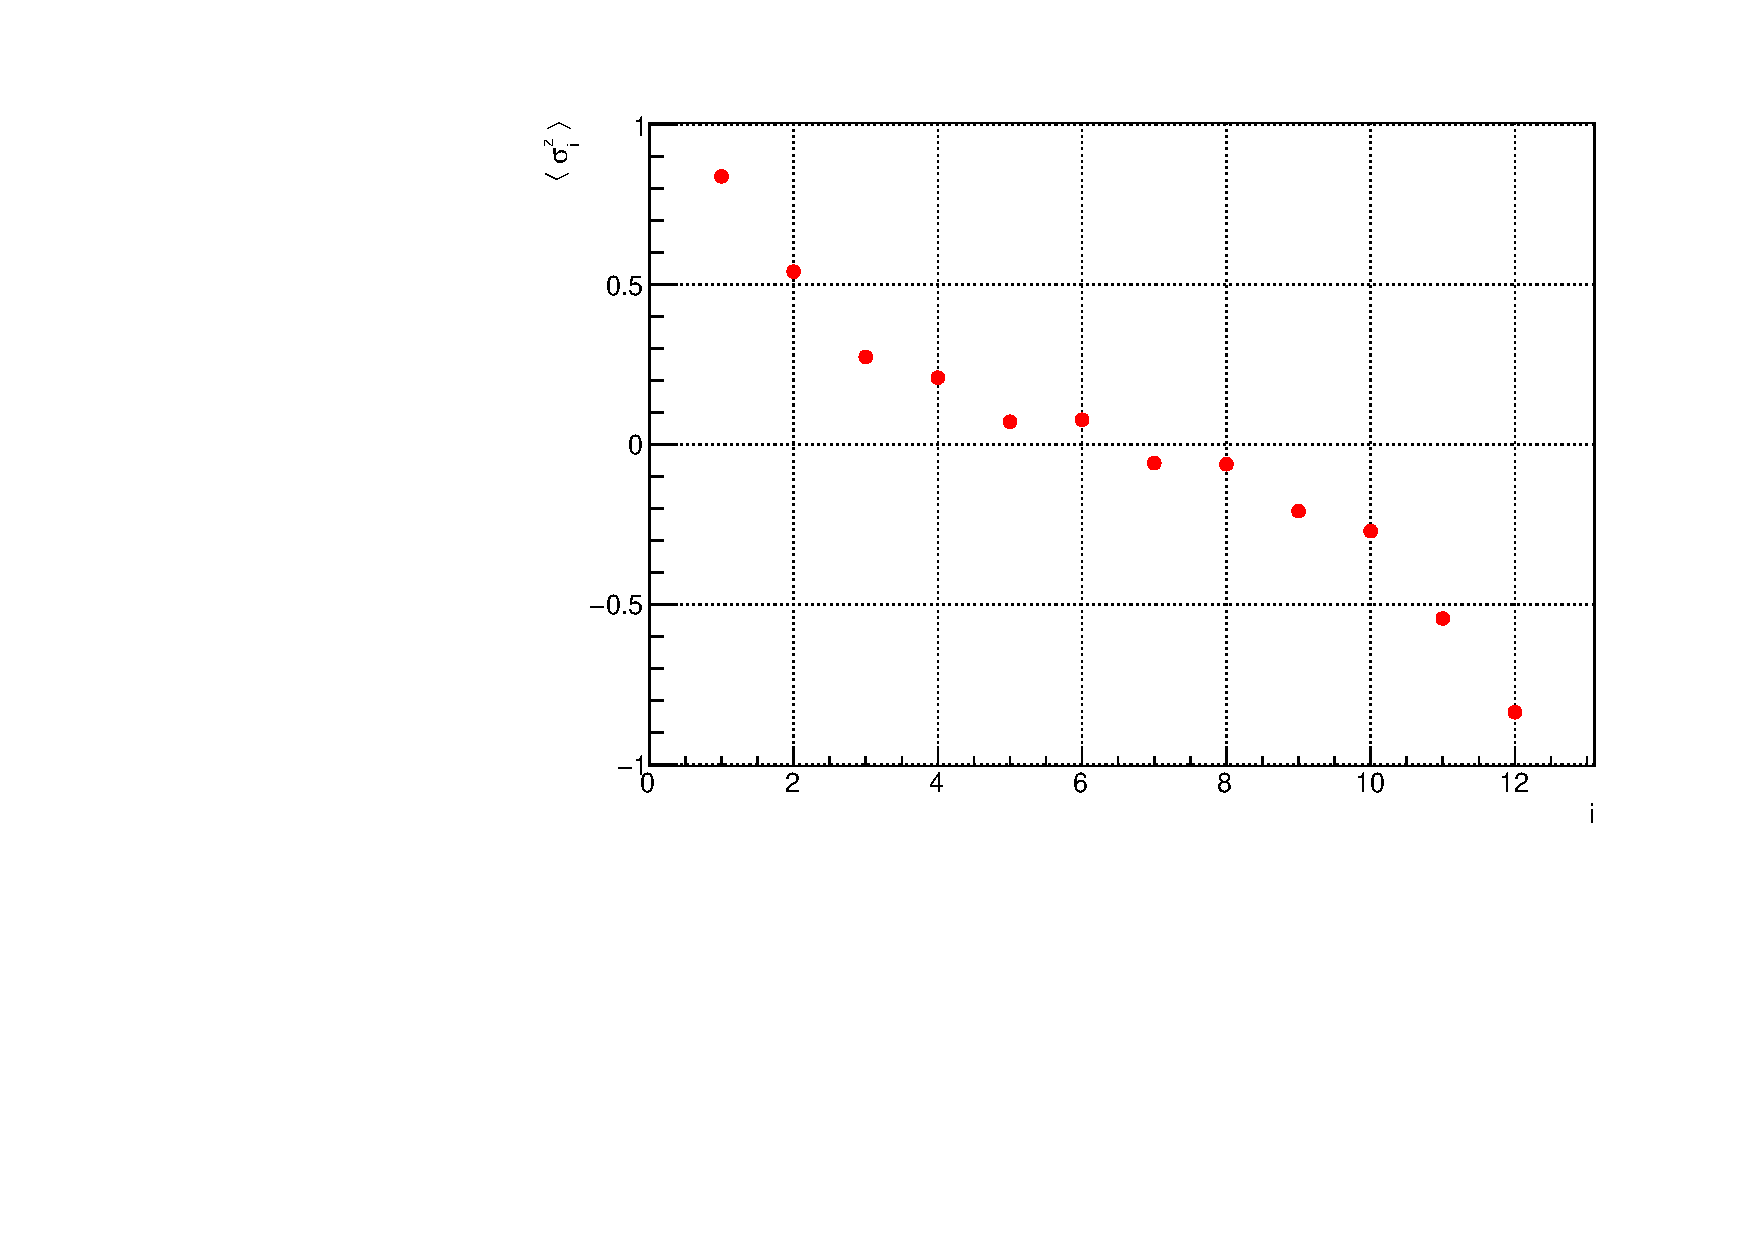
\includegraphics[scale=0.7]{Figures/12sites/LML012m060Time002000_J10515.pdf}
    \caption{Spin profile for a 12-sites chain characterized by $\gamma~=~1, J_x=1, J_y=0.5, J_z=1.5$. Data are obtained from MPO method, with m = 60 and T = 2000.}
    \label{fig:my_label}
\end{figure}

Let us see \textbf{16-sites} chain.

\begin{figure}[H]
    \centering
    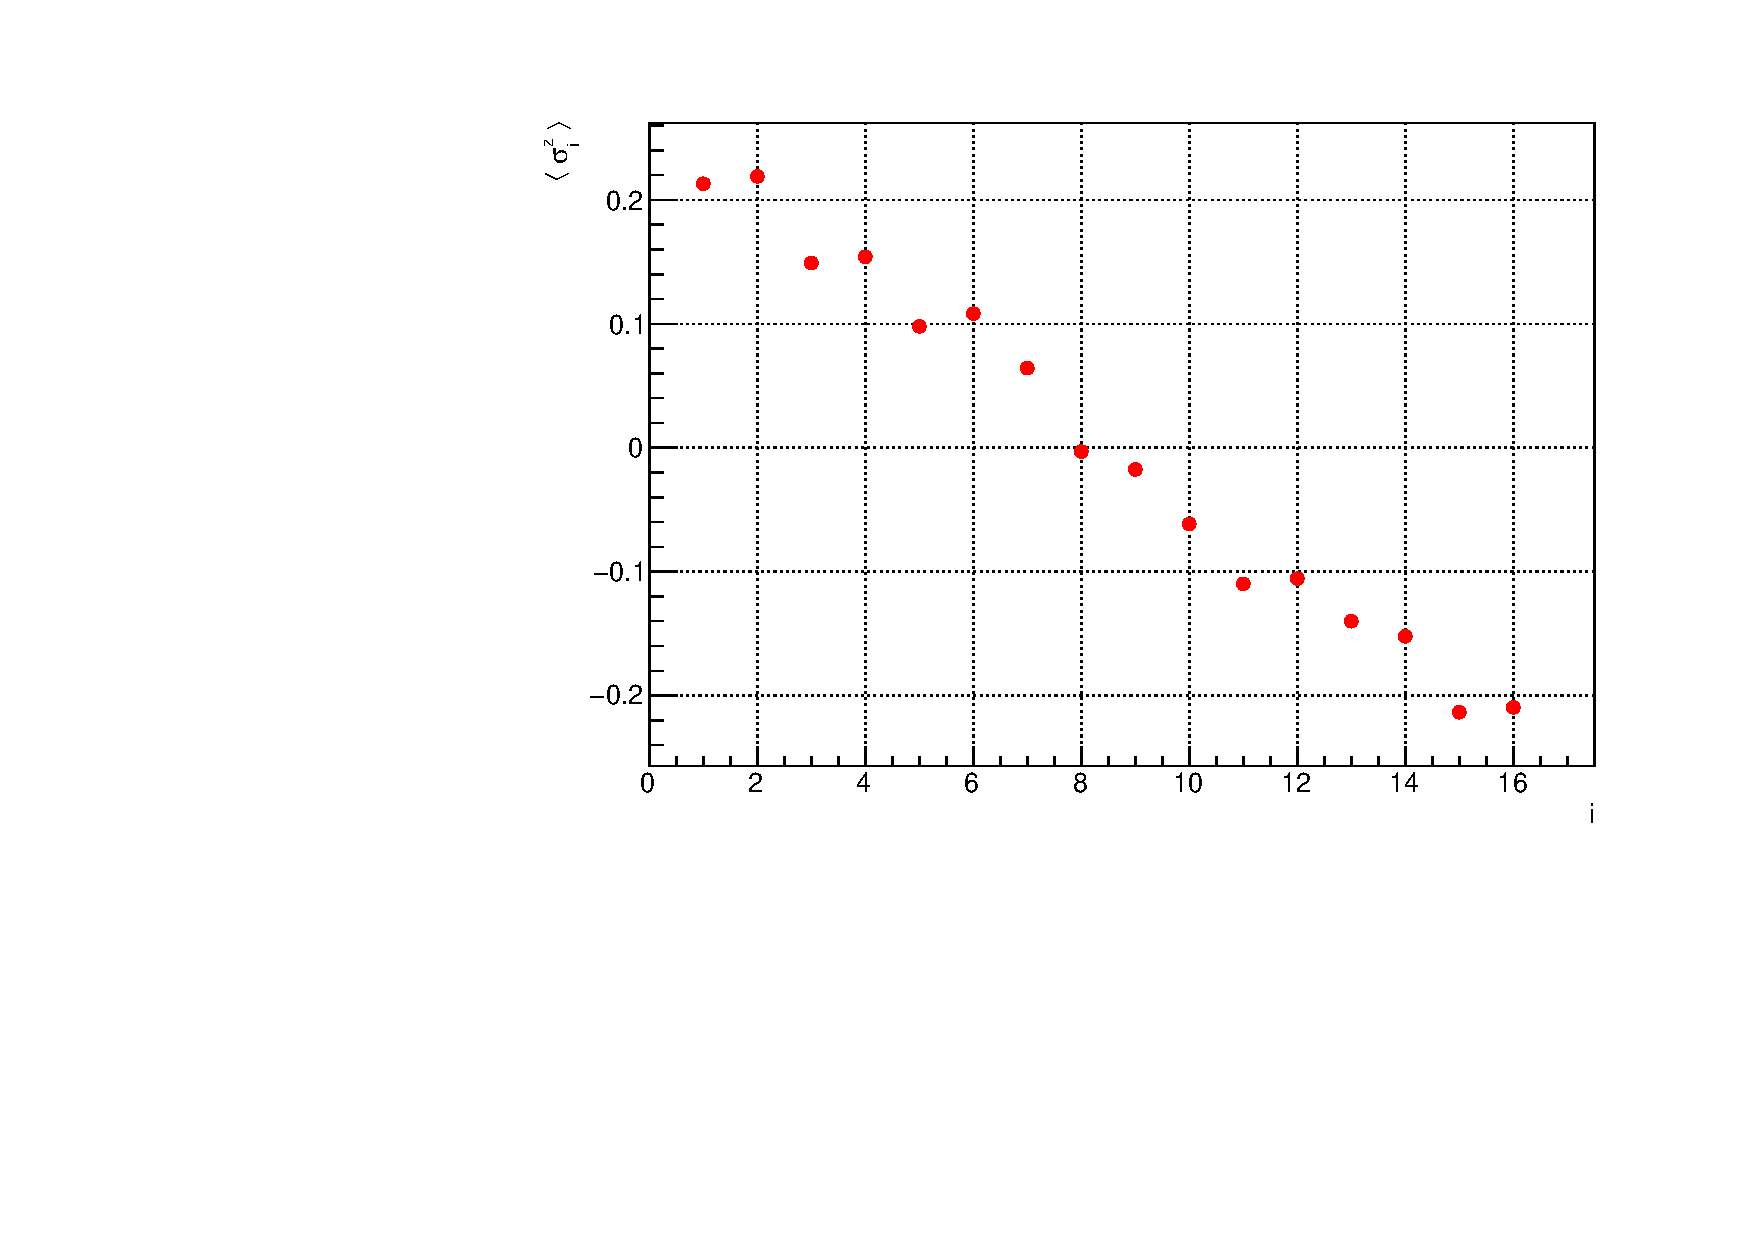
\includegraphics[scale=0.7]{Figures/16sites/LML016m080Time001000_J10505.pdf}
    \caption{Spin profile for a 16-sites chain characterized by $\gamma~=~1, J_x=1, J_y=0.5, J_z=0.5$. Data are obtained from MPO method, with m = 80 and T = 1000.}
    \label{fig:my_label}
\end{figure}

\begin{figure}[H]
    \centering
    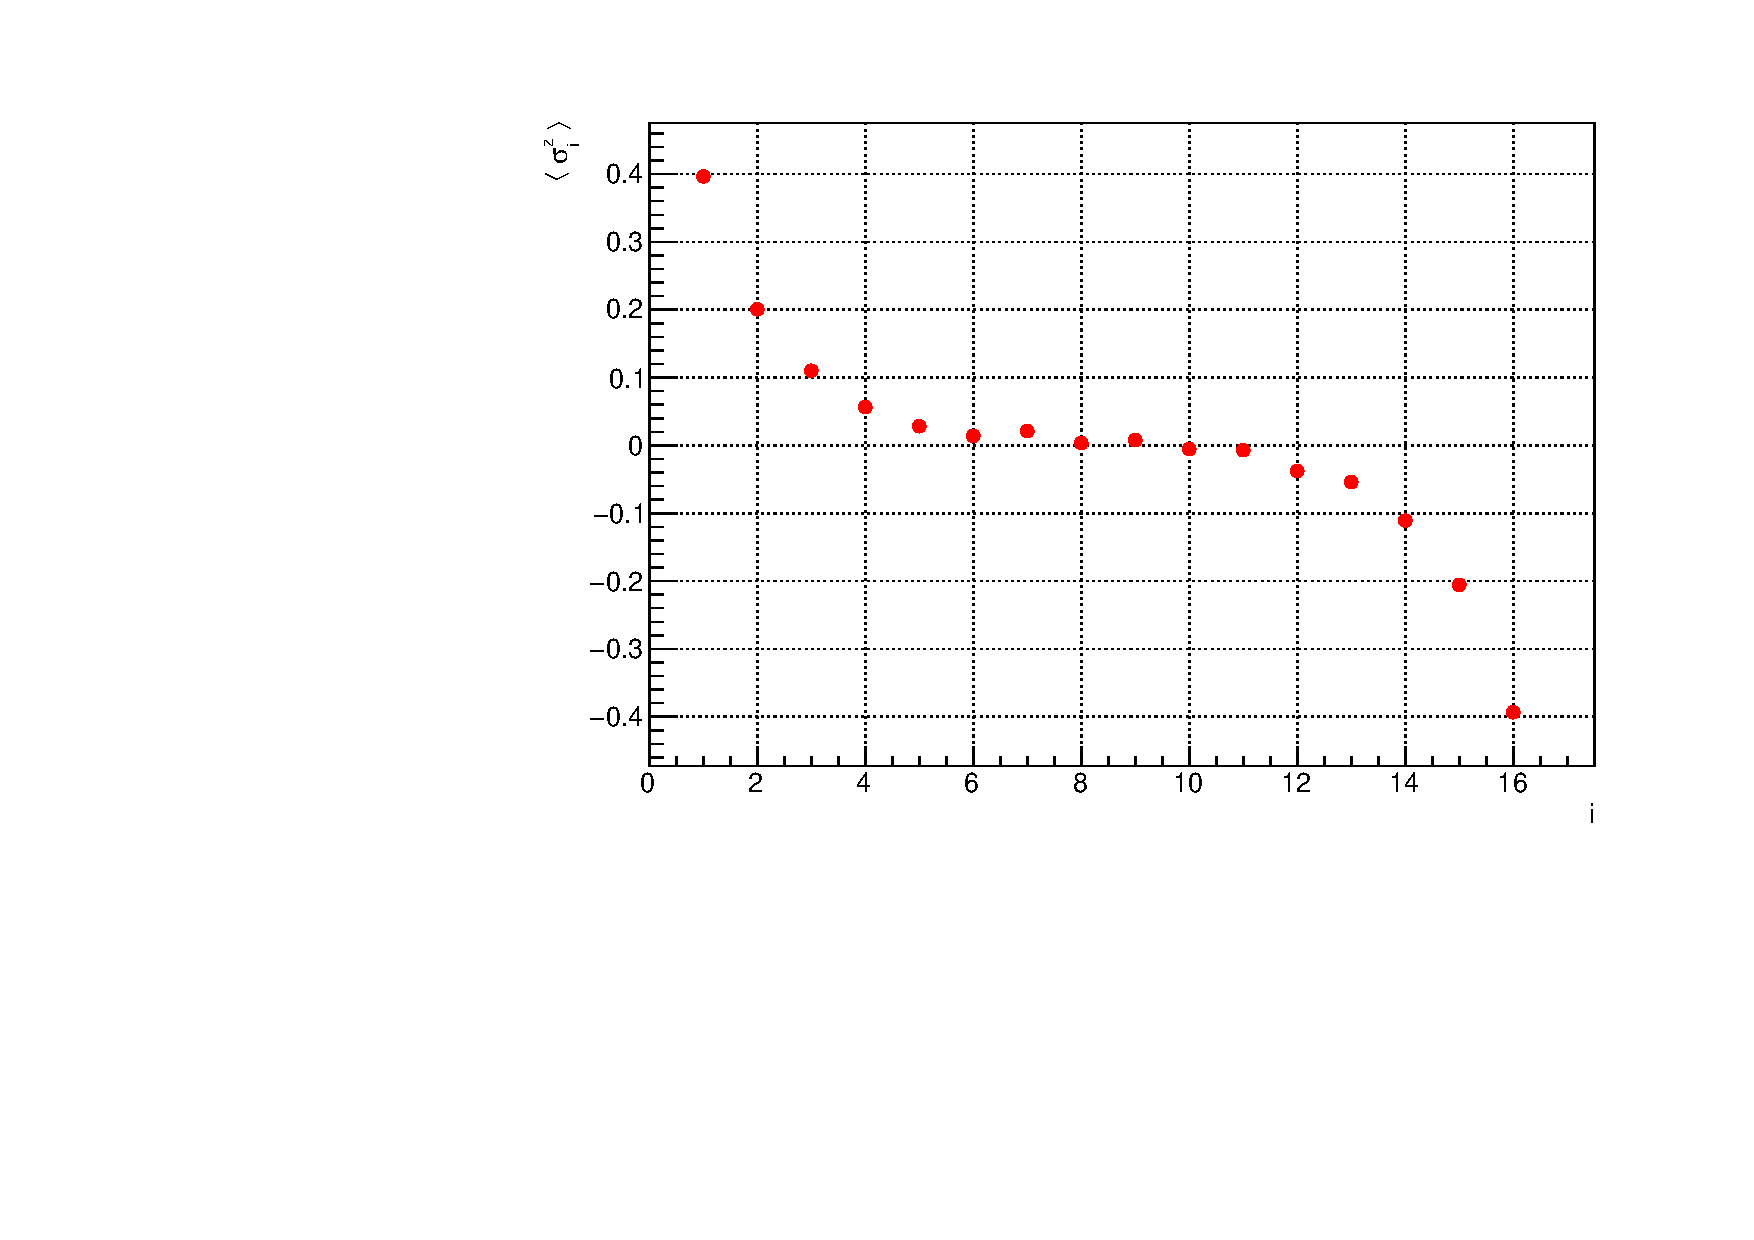
\includegraphics[scale=0.7]{Figures/16sites/LML016m080Time002500_J1051.pdf}
    \caption{Spin profile for a 16-sites chain characterized by $\gamma~=~1, J_x=1, J_y=0.5, J_z=1.$. Data are obtained from MPO method, with m = 80 and T = 2500.}
    \label{fig:my_label}
\end{figure}



In fig.~\ref{fig:LM_comparisonVSsizeJz1Gamma1} it is shown the comparison between the magnetization profile of chains with different lengths. Two characteristics stand out: the first one is the fact that the peak values of $\langle\sigma^z\rangle$ in the ends of the chain are independent from the size of the system; the second one involves the fact that increasing the length of the chain, the spin profile gets flatter.

\begin{figure}[H]
    \centering
    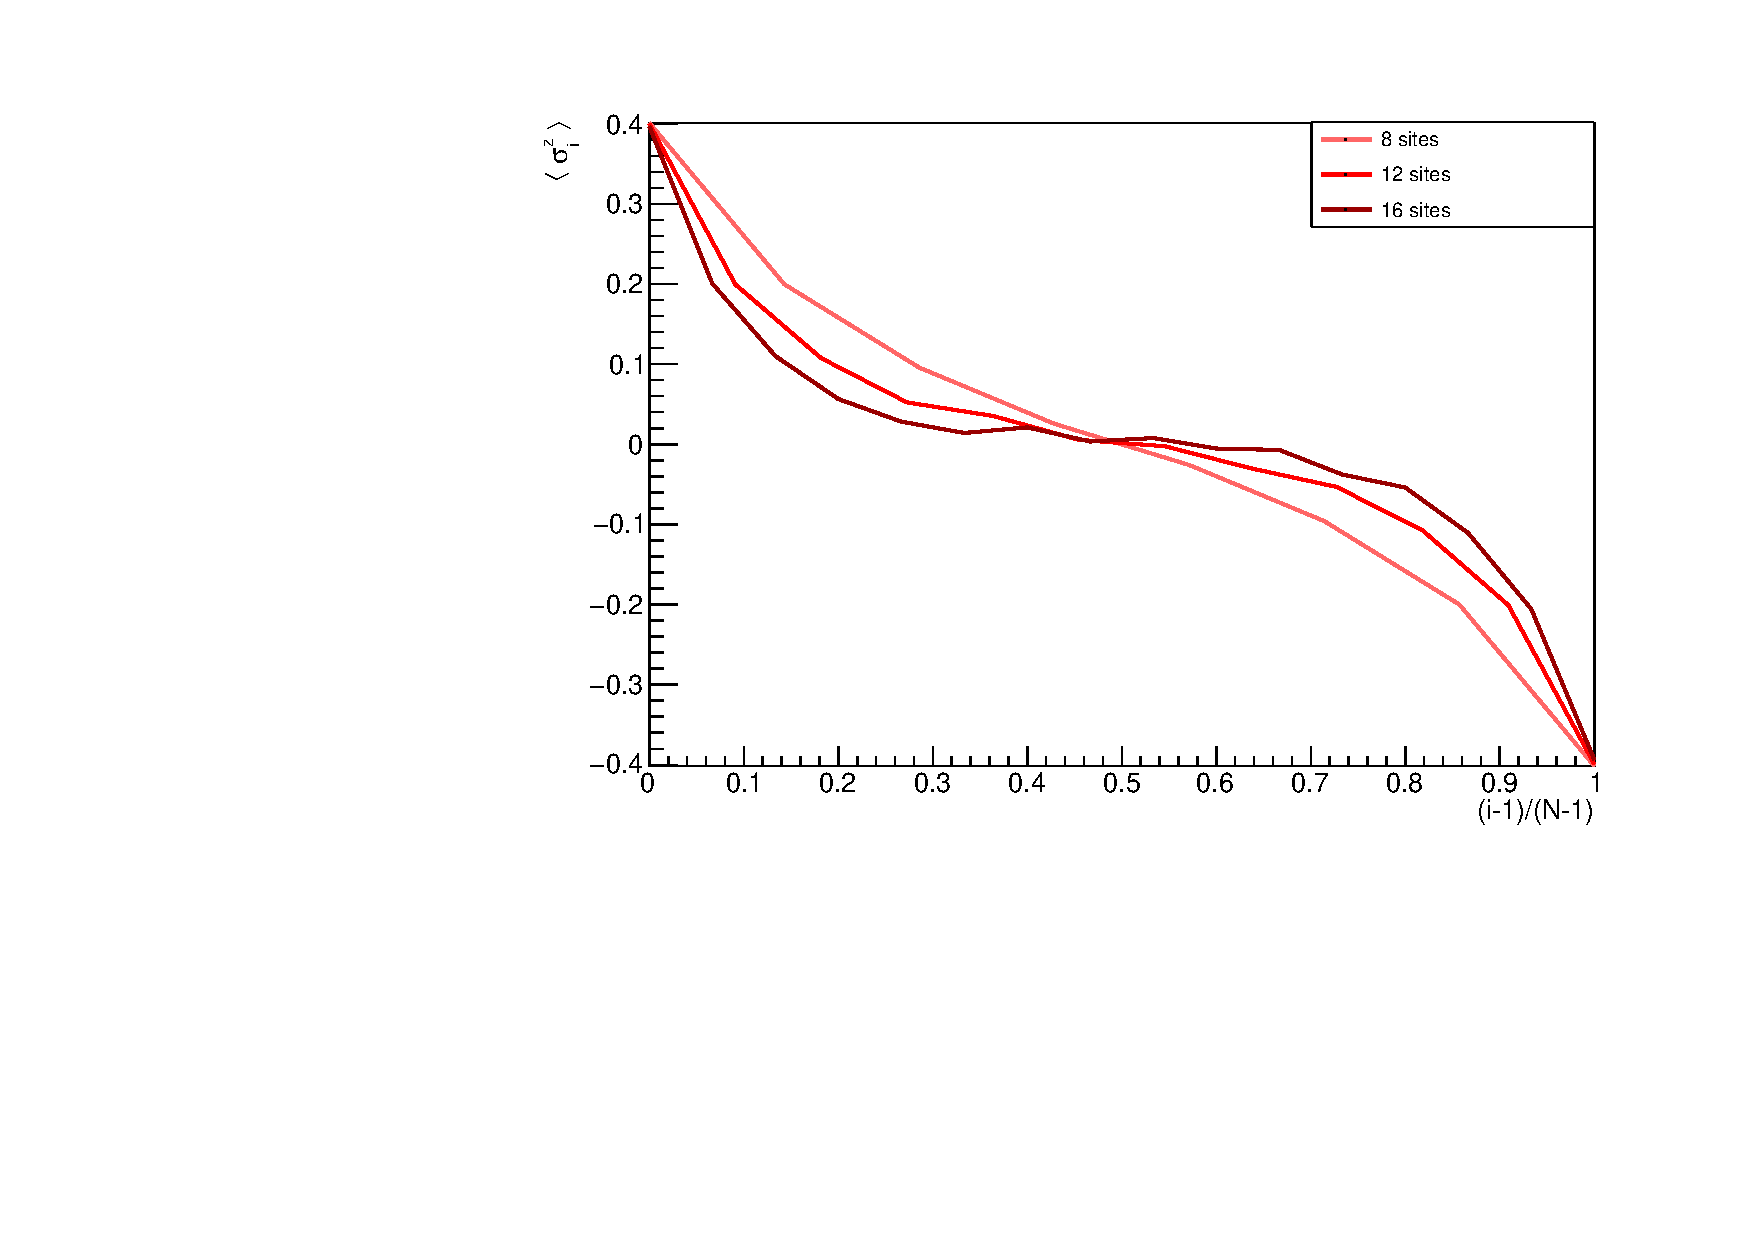
\includegraphics[scale=0.7]{Figures/NORM_LM_comparisonVSsize.pdf}
    \caption{Spin profile for the model under study at $J_z = 1$ and $\gamma=1$. Data for different chain length are shown and they are obtained from MPO method.}
    \label{fig:LM_comparisonVSsizeJz1Gamma1}
\end{figure}

In order to analyze these properties, we see how the behaviour of curves in fig.~\ref{fig:LM_comparisonVSsizeJz1Gamma1} change for different values of dissipation rate $\gamma$. This is shown in fig.\ref{fig:LMcompVSsizeANDdissRate}.

\begin{figure}[H]
    \centering
    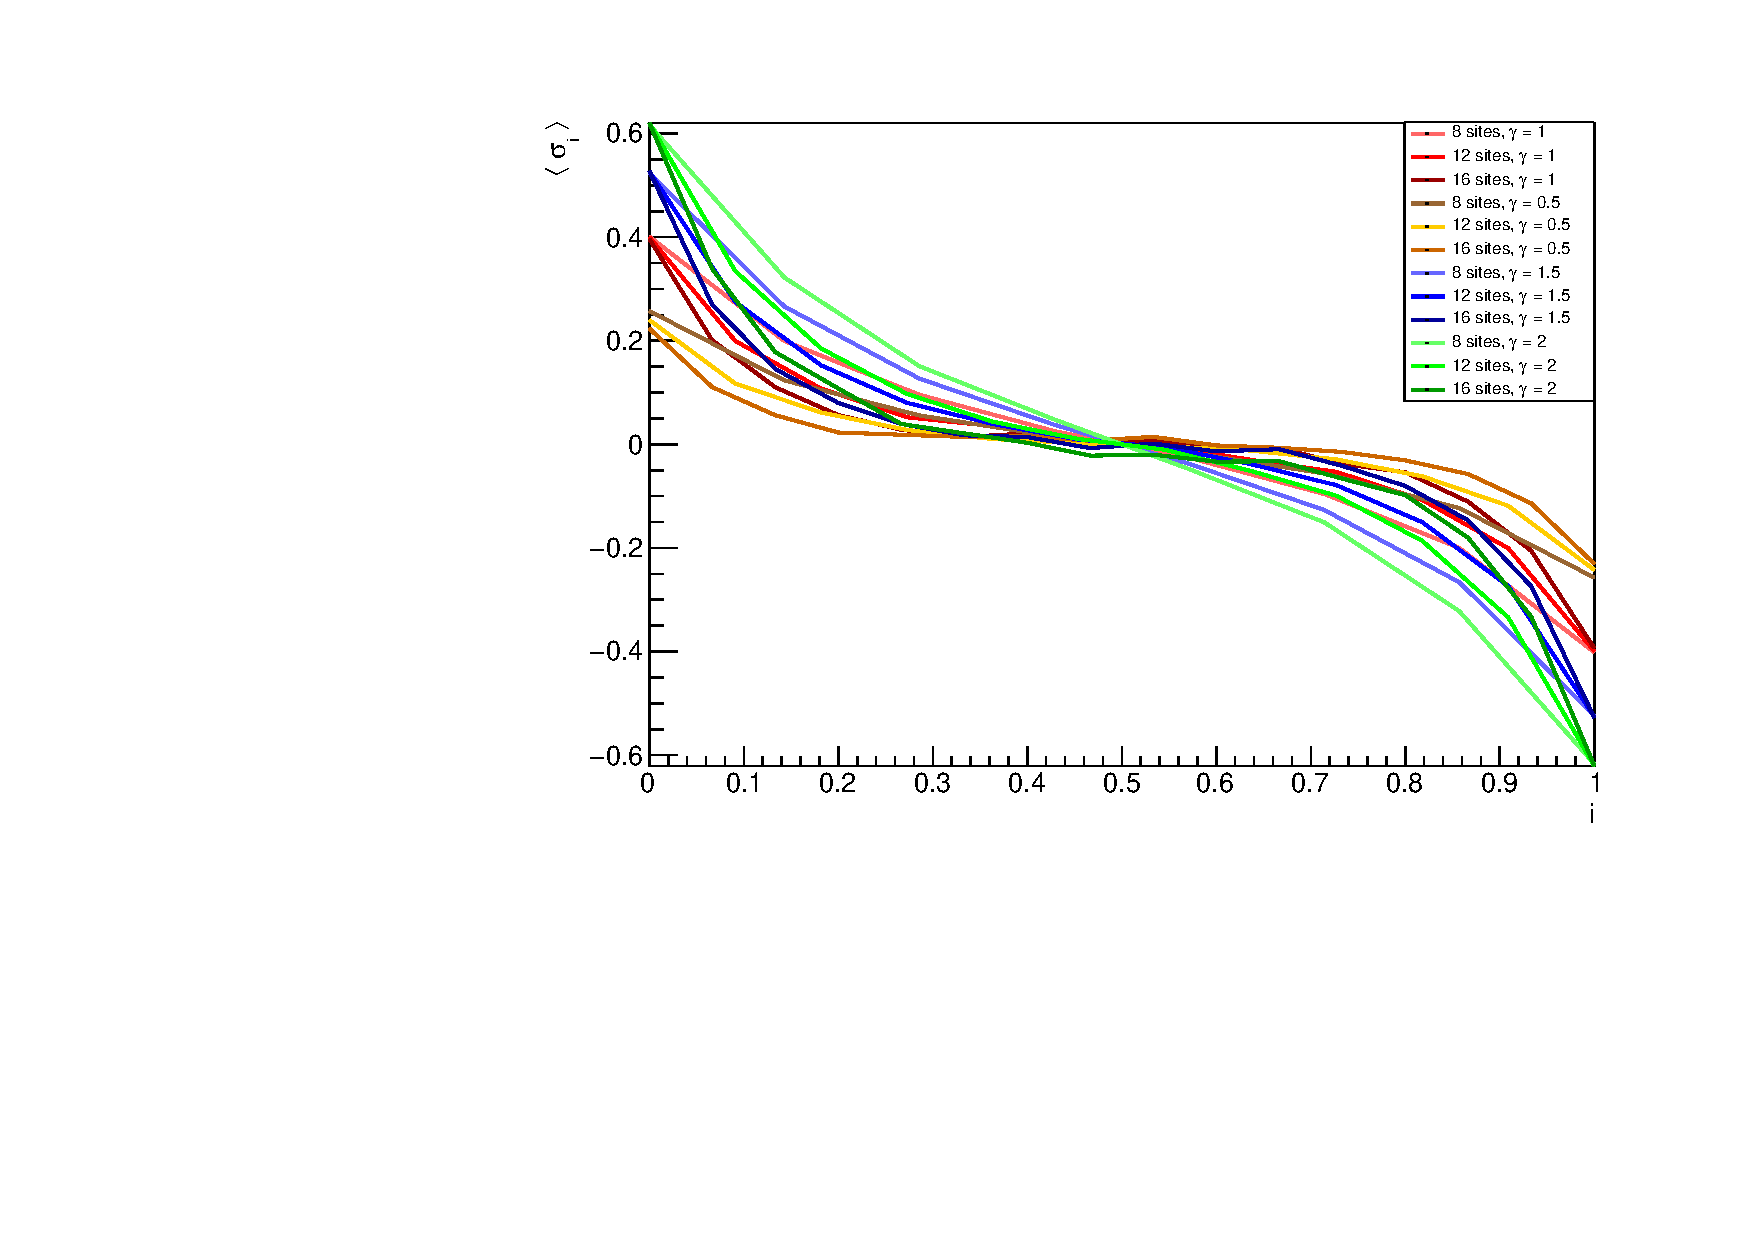
\includegraphics[scale=0.7]{Figures/LMcomparisonVSsizeANDdissipationRate.pdf}
    \caption{Spin profile for the model under study at $J_z = 1$ for several values of dissipation rate $\gamma$. It seems clear that while $\gamma$ decreases the profile gets flatter. Data are obtained from MPO method.\textcolor{red}{\\DO IT AGAIN!}}
    \label{fig:LMcompVSsizeANDdissRate}
\end{figure}

Here, it seems clear that while increasing $\gamma$, the ends of the chain becomes more and more polarized. In addition to this, we can anticipate that for bigger values of $\gamma$, for a fixed size of the chain, the spin profile gets flatter. This behaviour will be analyzed in greater detail in the following.

First of all, it is convenient separate the curves for each size (8, 12 and 16 sites) in order to distinguish the profiles. The plots are shown below.

\begin{figure}[H]
    \centering
    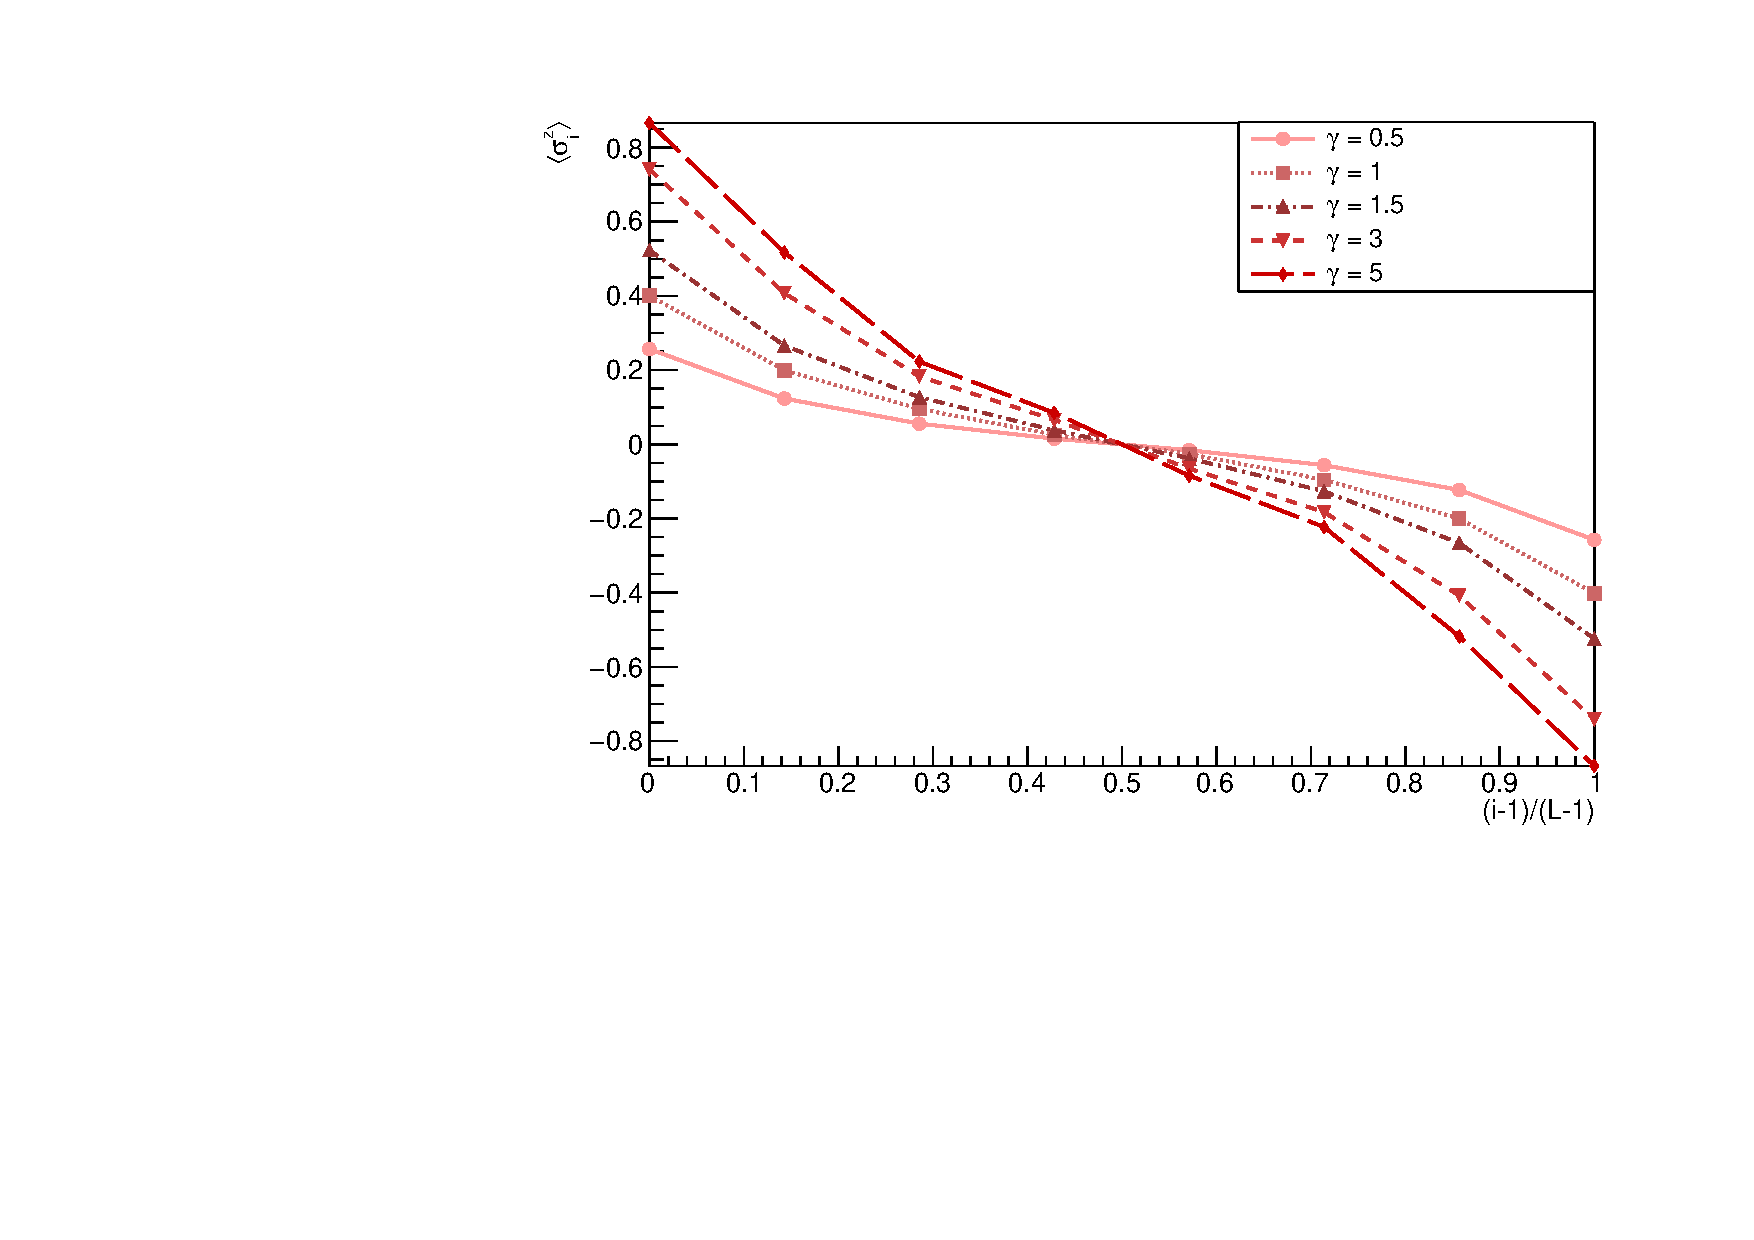
\includegraphics[scale=0.7]{Figures/8sites/8sites_LMvsGamma.pdf}
    \caption{Spin profile for a 8-sites chain varying on dissipation rate $\gamma$. Data are obtained from MPO method.}
    \label{fig:8sites_LMvsGamma}
\end{figure}

\begin{figure}[H]
    \centering
    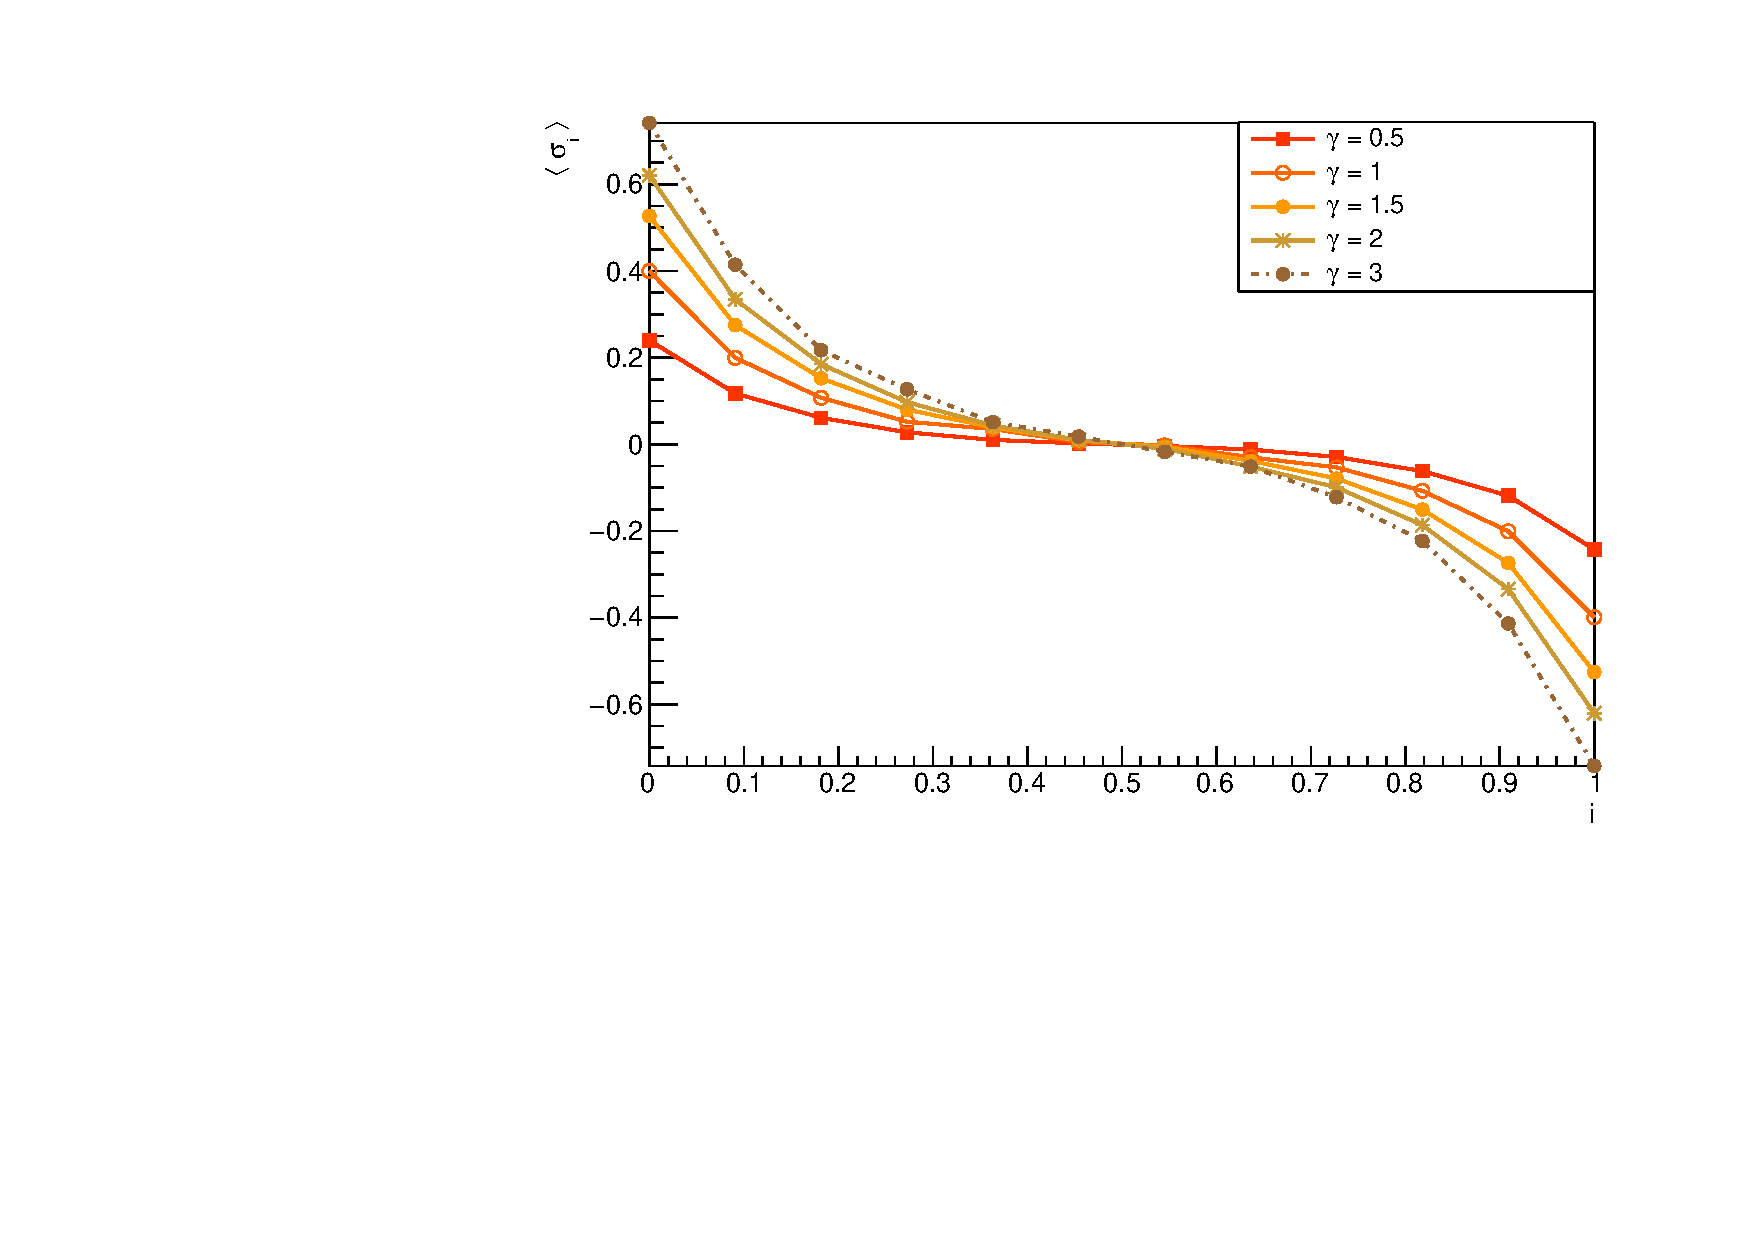
\includegraphics[scale=0.7]{Figures/12sites/12sites_LMvsGamma.pdf}
    \caption{Spin profile for a 12-sites chain varying on dissipation rate $\gamma$. Data are obtained from MPO method.}
    \label{fig:12sites_LMvsGamma}
\end{figure}

\begin{figure}[H]
    \centering
    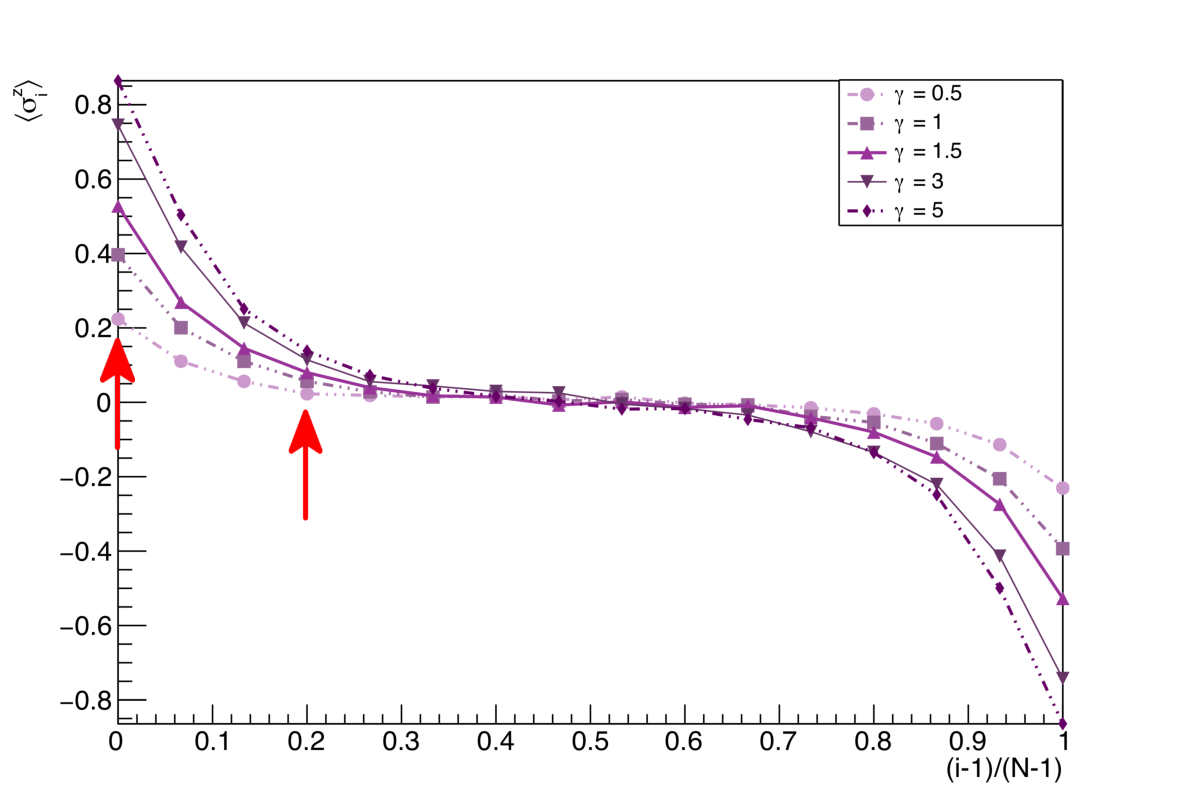
\includegraphics[scale=0.7]{Figures/16sites/16sites_LMvsGamma.pdf}
    \caption{Spin profile for a 16-sites chain varying on dissipation rate $\gamma$. Data are obtained from MPO method.}
    \label{fig:16sites_LMvsGamma}
\end{figure}

As said previously, the peak value of $\langle\sigma^z\rangle$ varies with $\gamma$. In the fig.~\ref{fig:FIT_PeakLMvsGamma_J1051} it is presented the fit~\cite{root_cern} that shows an exponential behaviour. 

\begin{figure}[H]
    \centering
    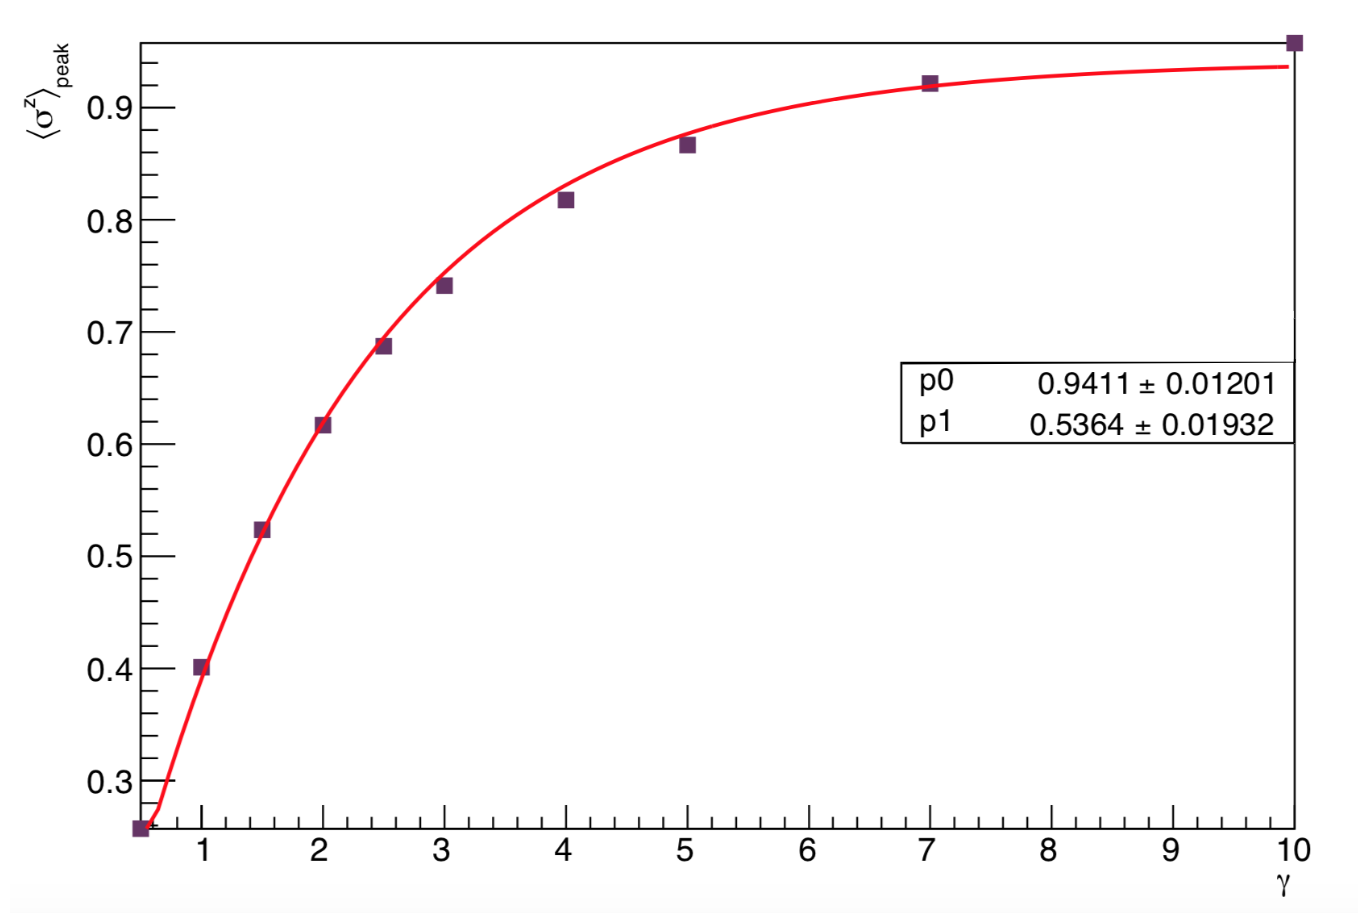
\includegraphics[scale=0.5]{Figures/FIT_PeakLMVsGamma.png}
    \caption{The red line shows the fit $\langle\sigma^z\rangle_{max} = p_0(1-e^{-p_1\gamma})$.}
    \label{fig:FIT_PeakLMvsGamma_J1051}
\end{figure}

It is interesting noting that the same dependence is keep also by $\langle\sigma^z\rangle$ of spins lying in the $\frac{N}{4}$-th site, as shown in fig.\ref{fig:FIT8sites_LM_2ndSiteVSgamma}, \ref{fig:FIT12sites_3rdSiteVSgamma}, \textcolor{red}{16SITES IS MISSING, TO DO}

\begin{figure}[H]
    \centering
    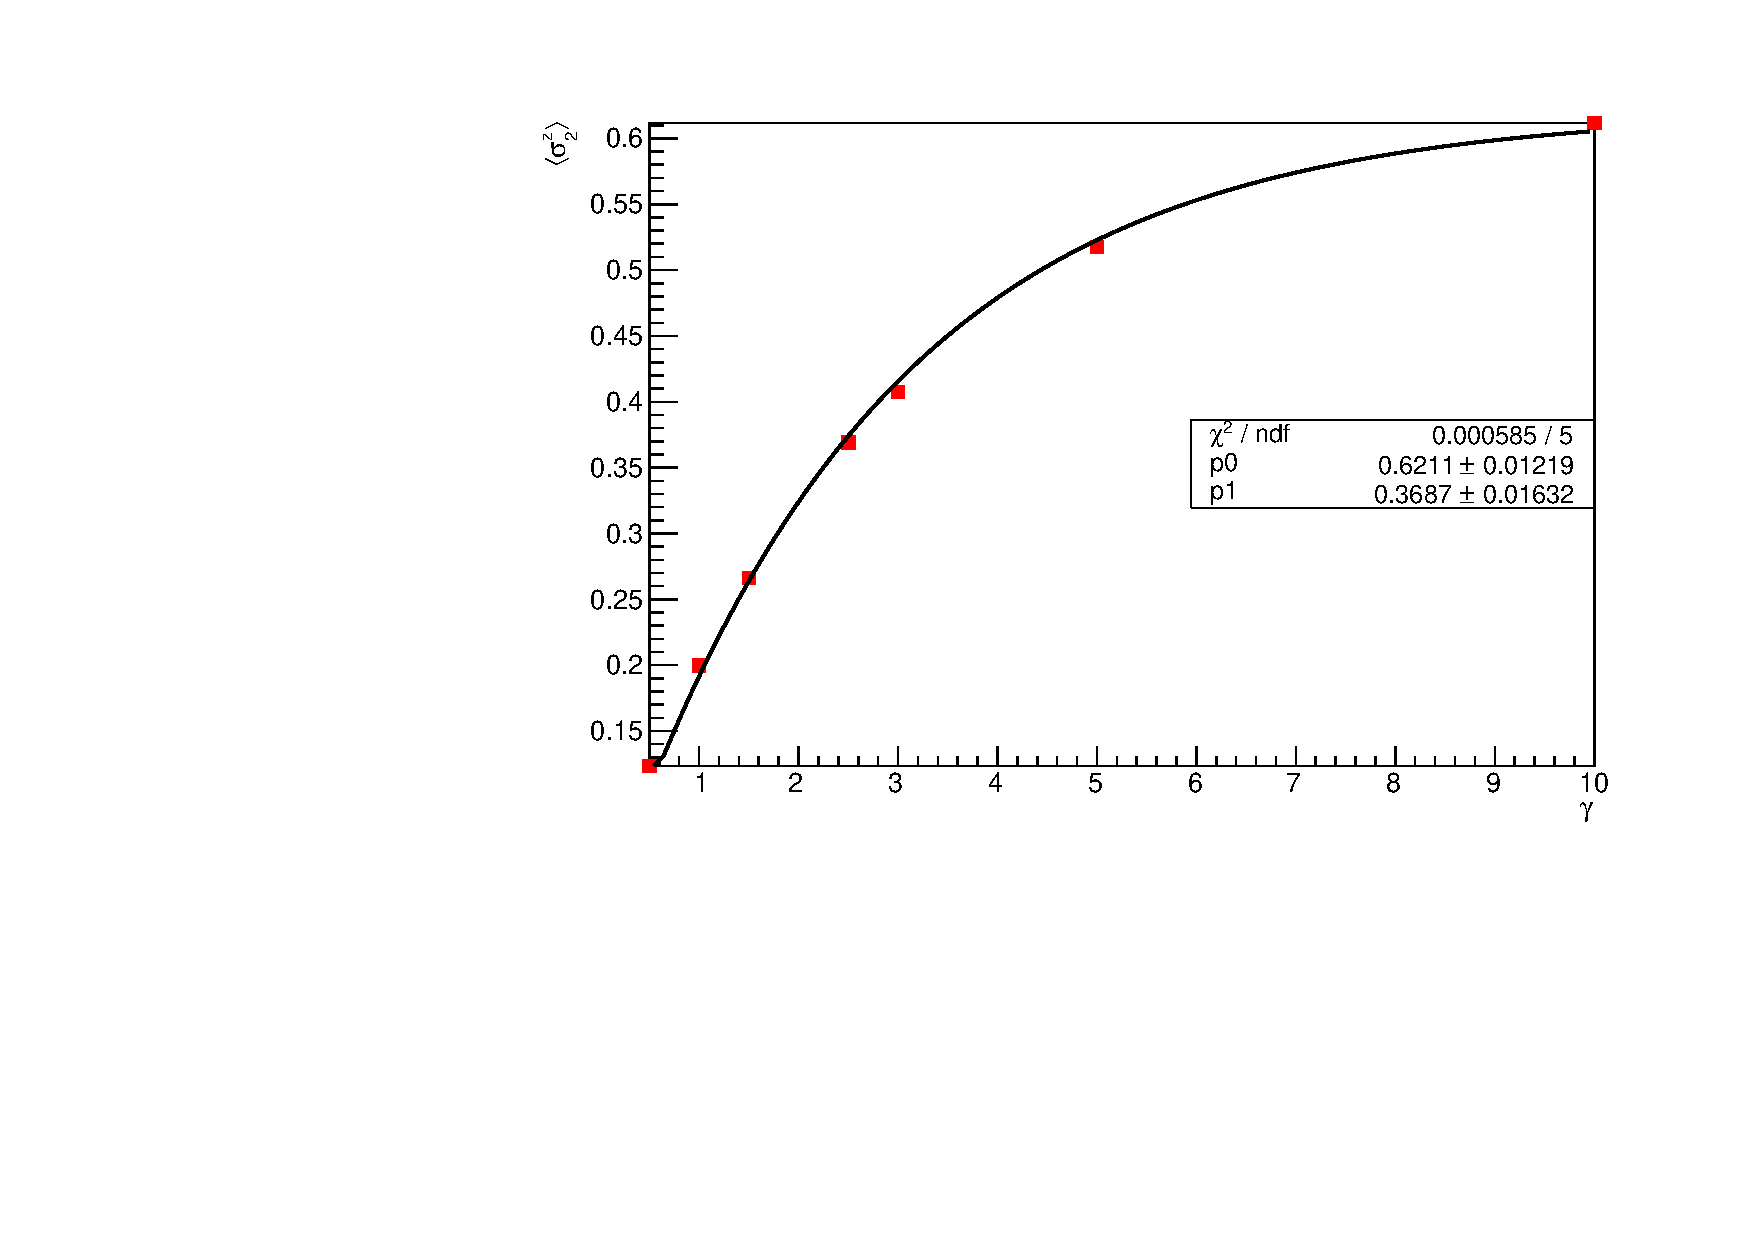
\includegraphics[scale=0.7]{Figures/8sites/FIT_8sites_2ndLMvsGamma.pdf}
    \caption{8 sites, the black line shows the fit \\$\langle\sigma^z\rangle_{peak}(\gamma) = p_0(1-e^{-p_1\gamma})$.}
    \label{fig:FIT8sites_LM_2ndSiteVSgamma}
\end{figure}

\begin{figure}[H]
    \centering
    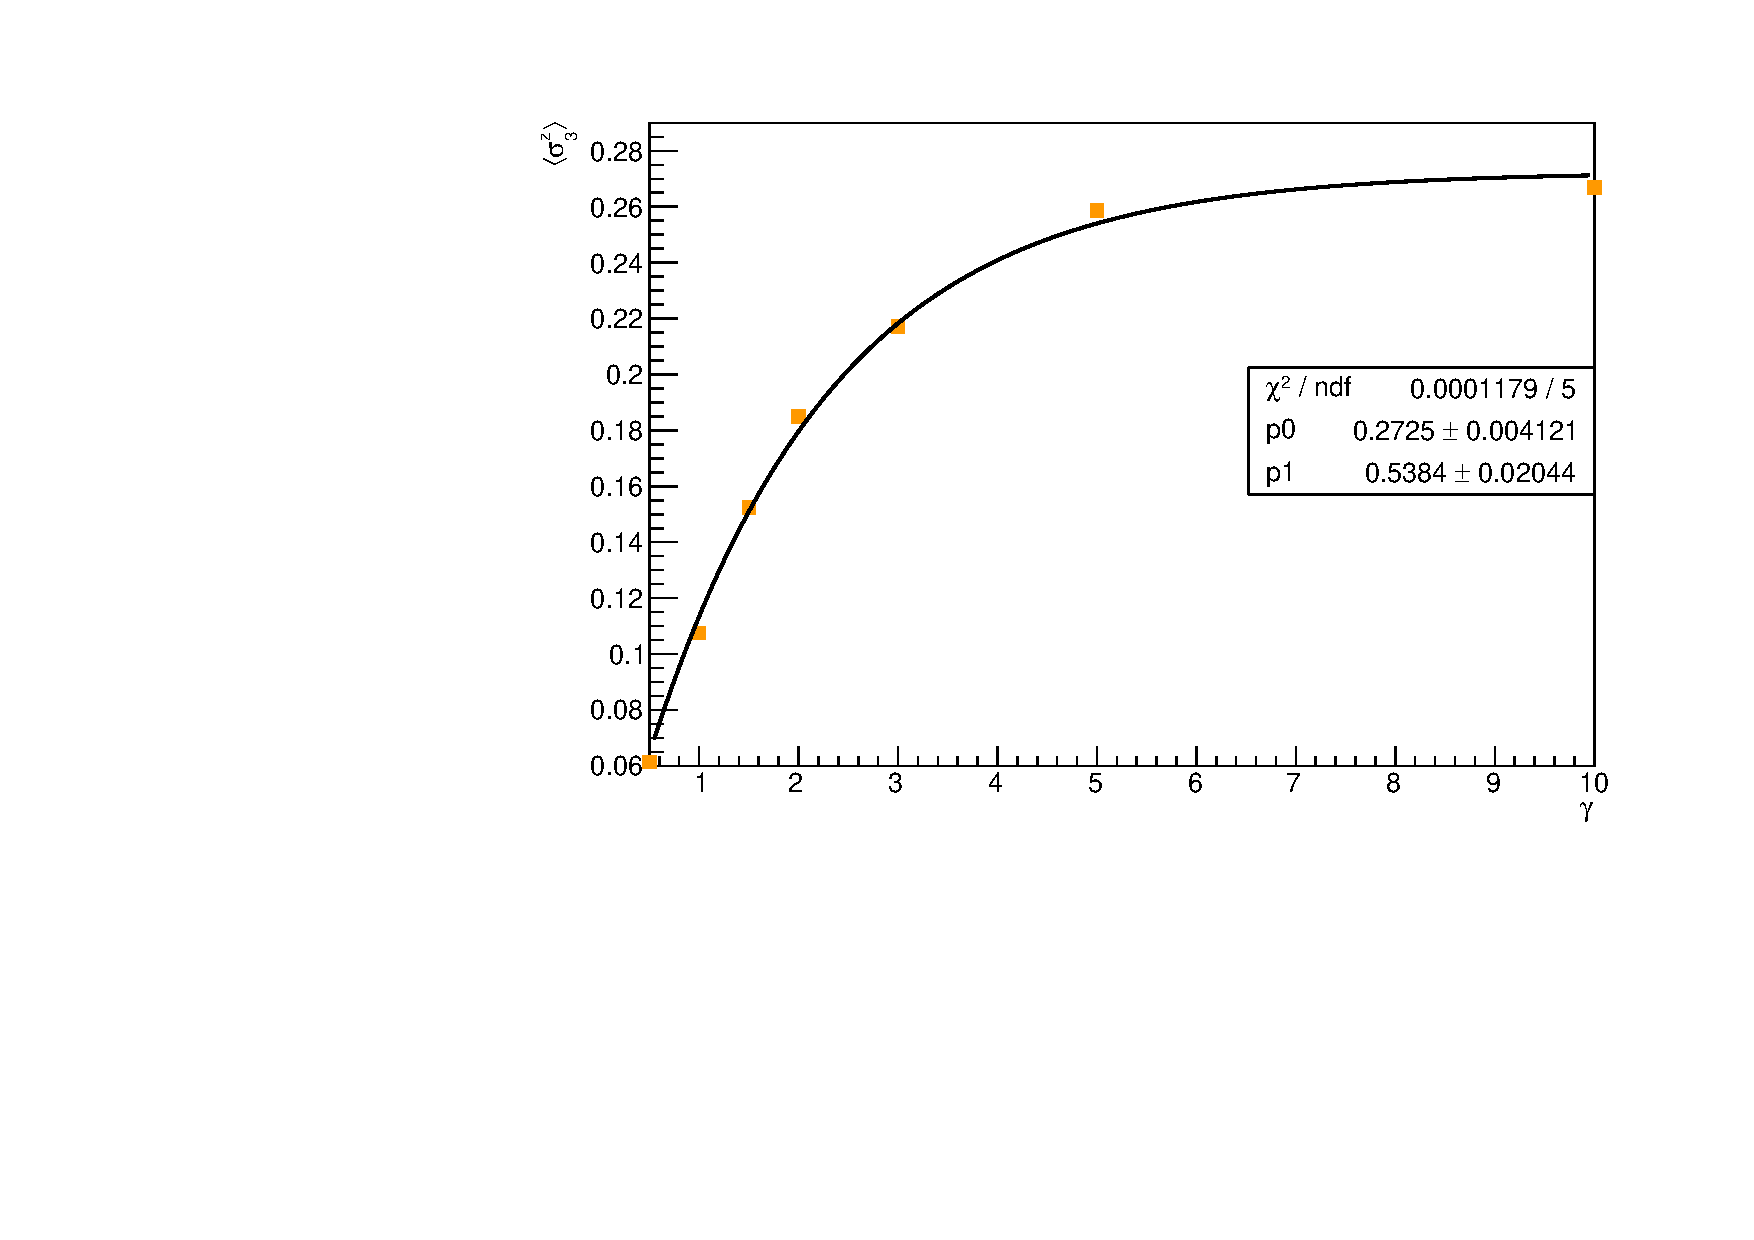
\includegraphics[scale=0.7]{Figures/12sites/FIT_12sites_3rdLMvsGamma.pdf}
    \caption{12 sites, the black line shows the fit \\$\langle\sigma^z\rangle_{peak}(\gamma) = p_0(1-e^{-p_1\gamma})$.}
    \label{fig:FIT12sites_3rdSiteVSgamma}
\end{figure}

Now let us study the gradient of magnetization for some site of the chain varying $\gamma$. The plots shown below are \textcolor{red}{WHAT}

\begin{figure}[H]
    \centering
    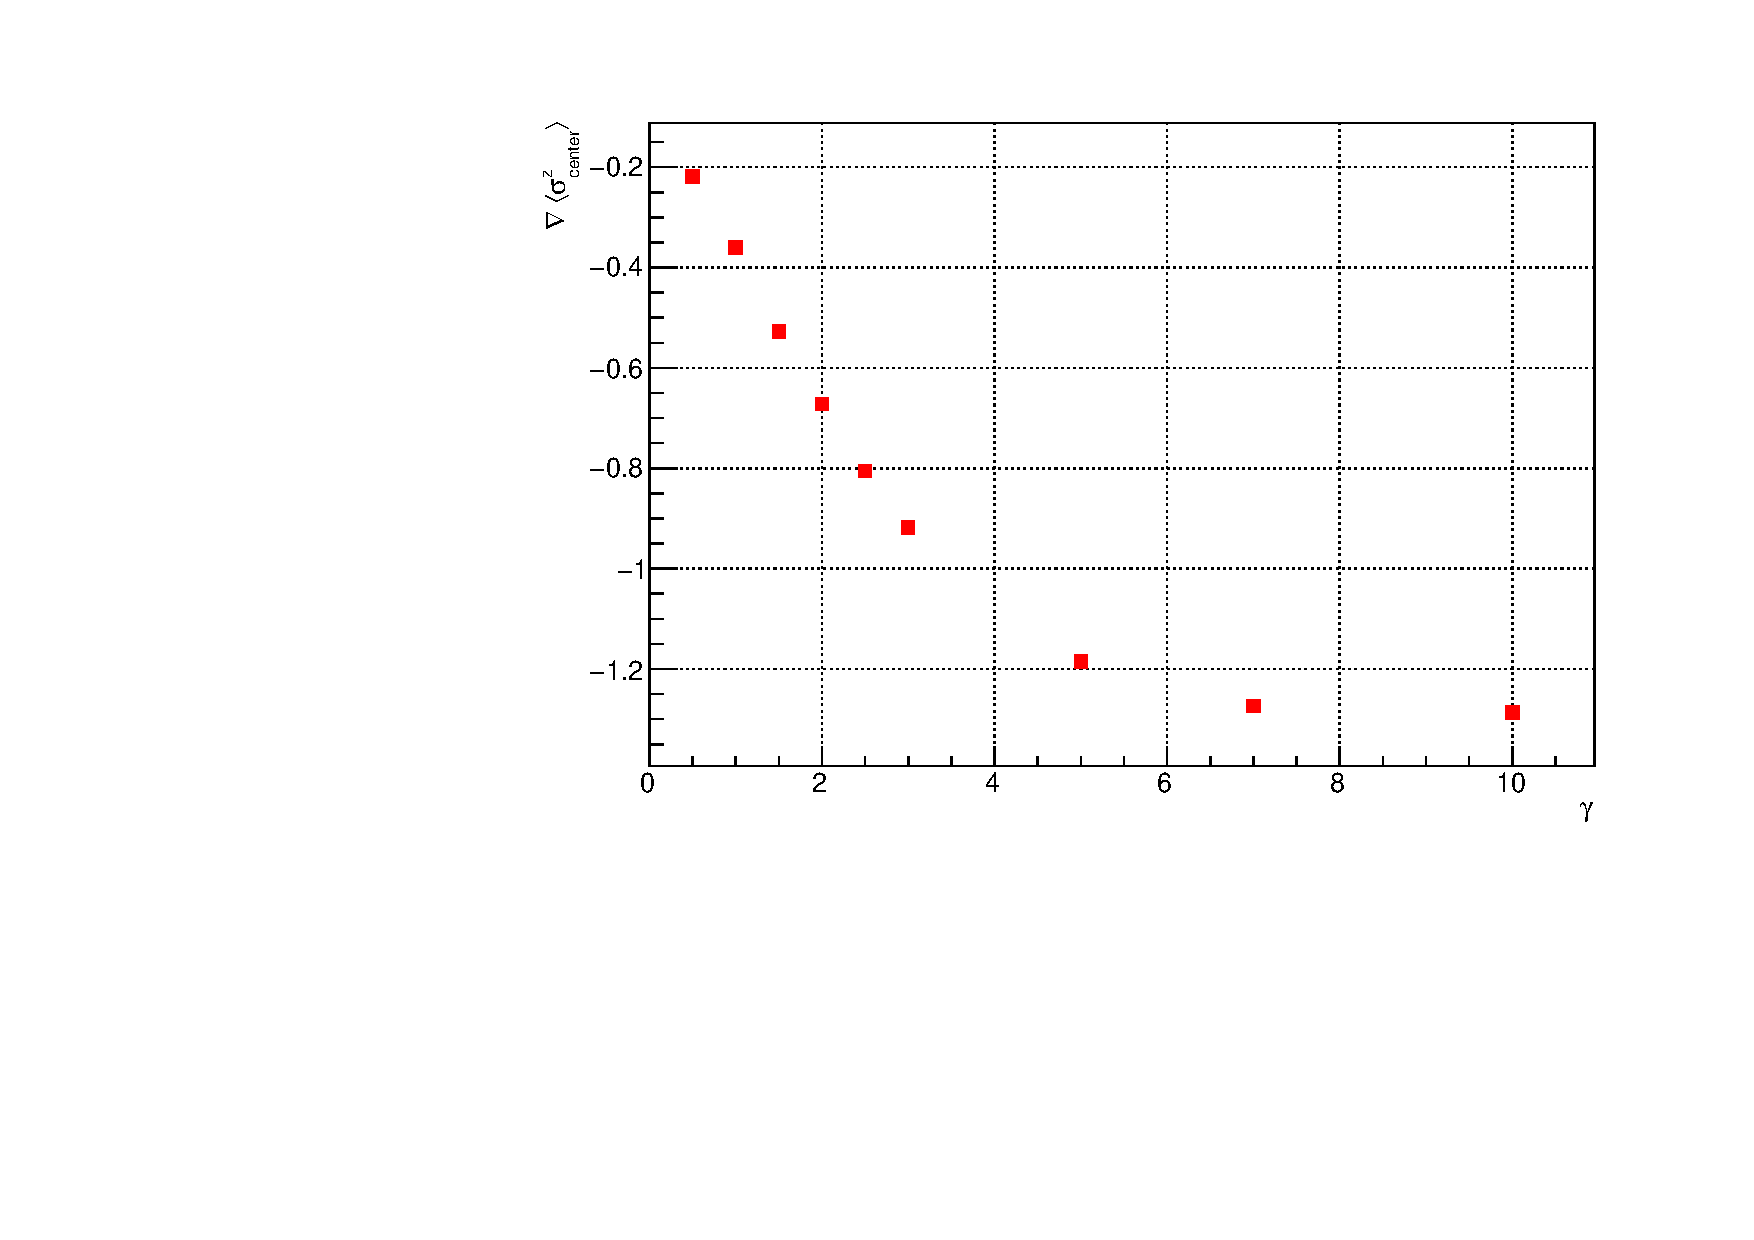
\includegraphics[scale=0.7]{Figures/8sites_comparison/8sites_gradLM_centerChainVSgamma.pdf}
    \caption{\textcolor{red}{FIT}}
    \label{fig:my_label}
\end{figure}

\begin{figure}[H]
    \centering
    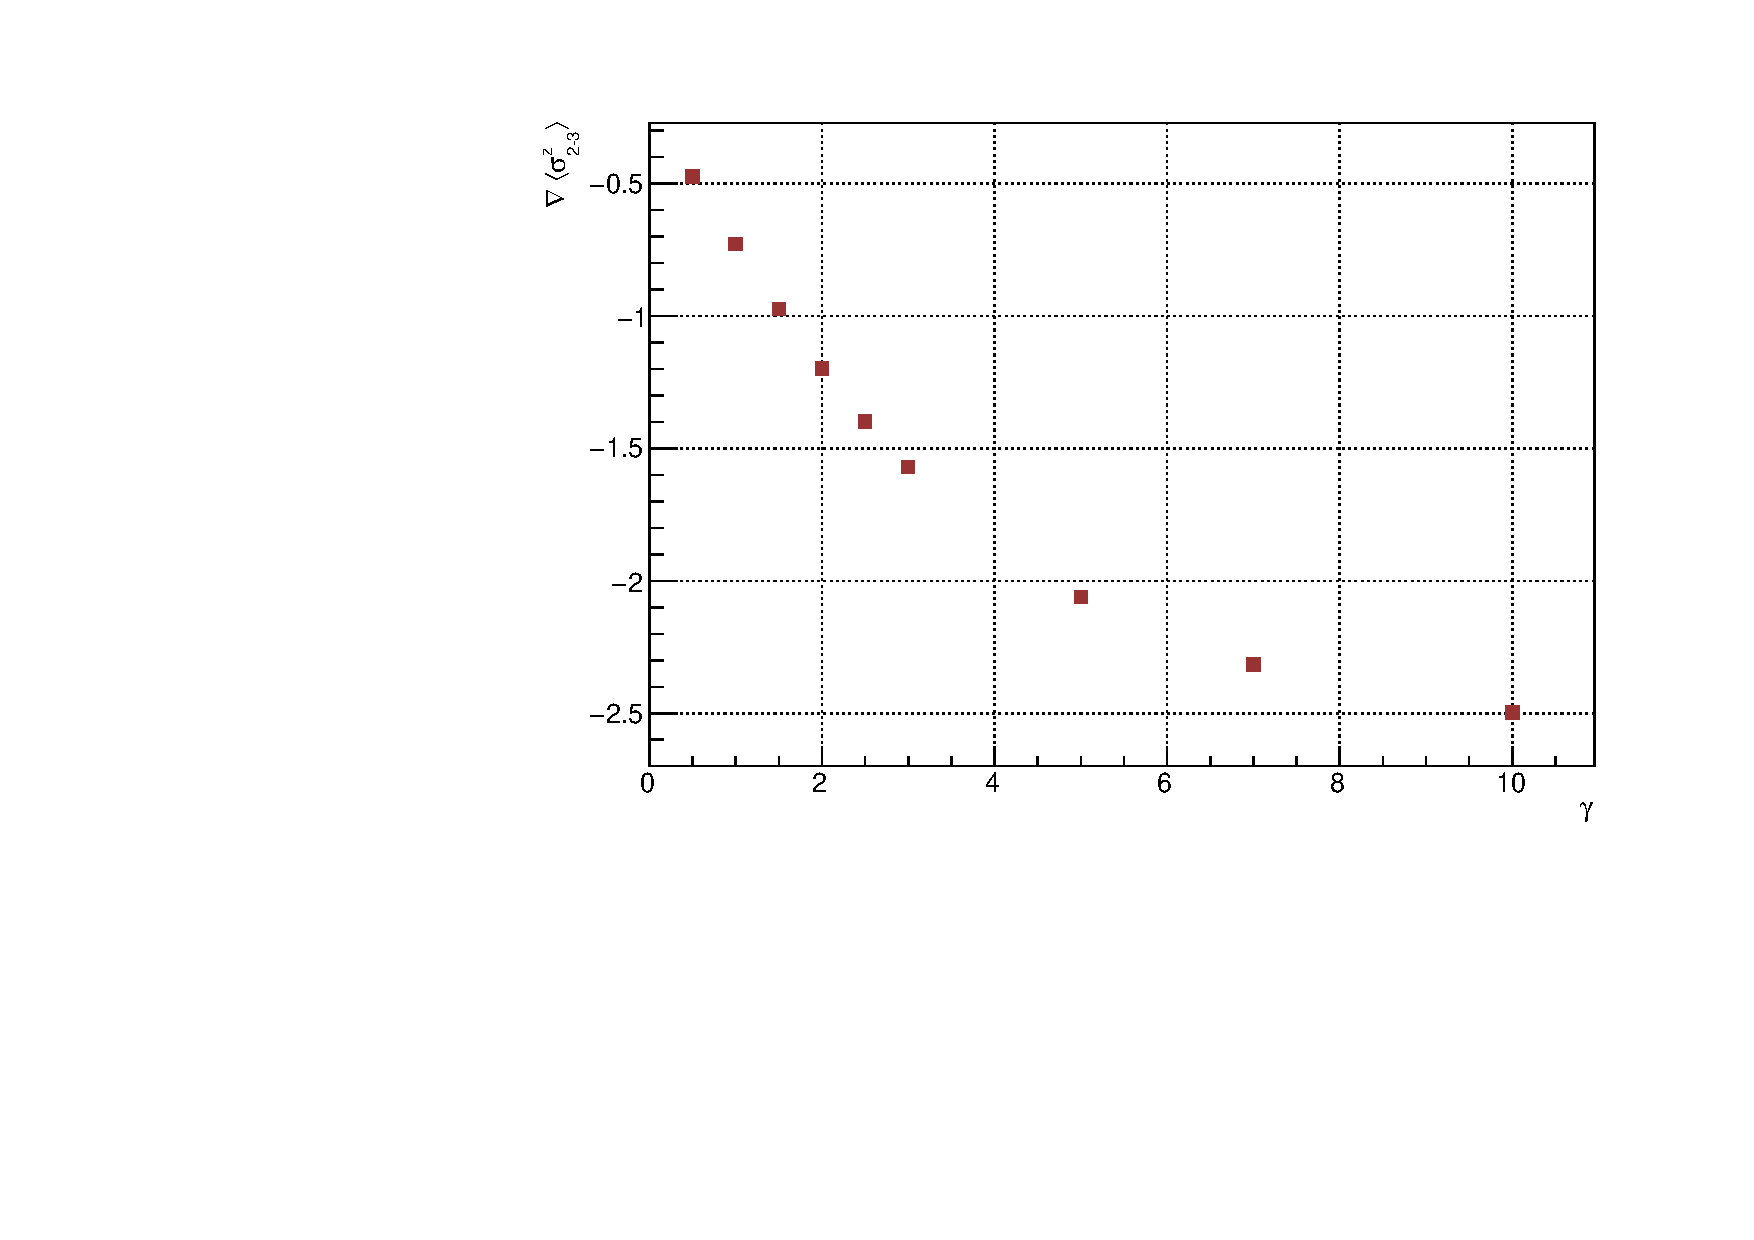
\includegraphics[scale=0.7]{Figures/8sites_comparison/8sites_gradLM_2and3VSgamma.pdf}
    \caption{\textcolor{red}{FIT}}
    \label{fig:my_label}
\end{figure}

\begin{figure}[H]
    \centering
    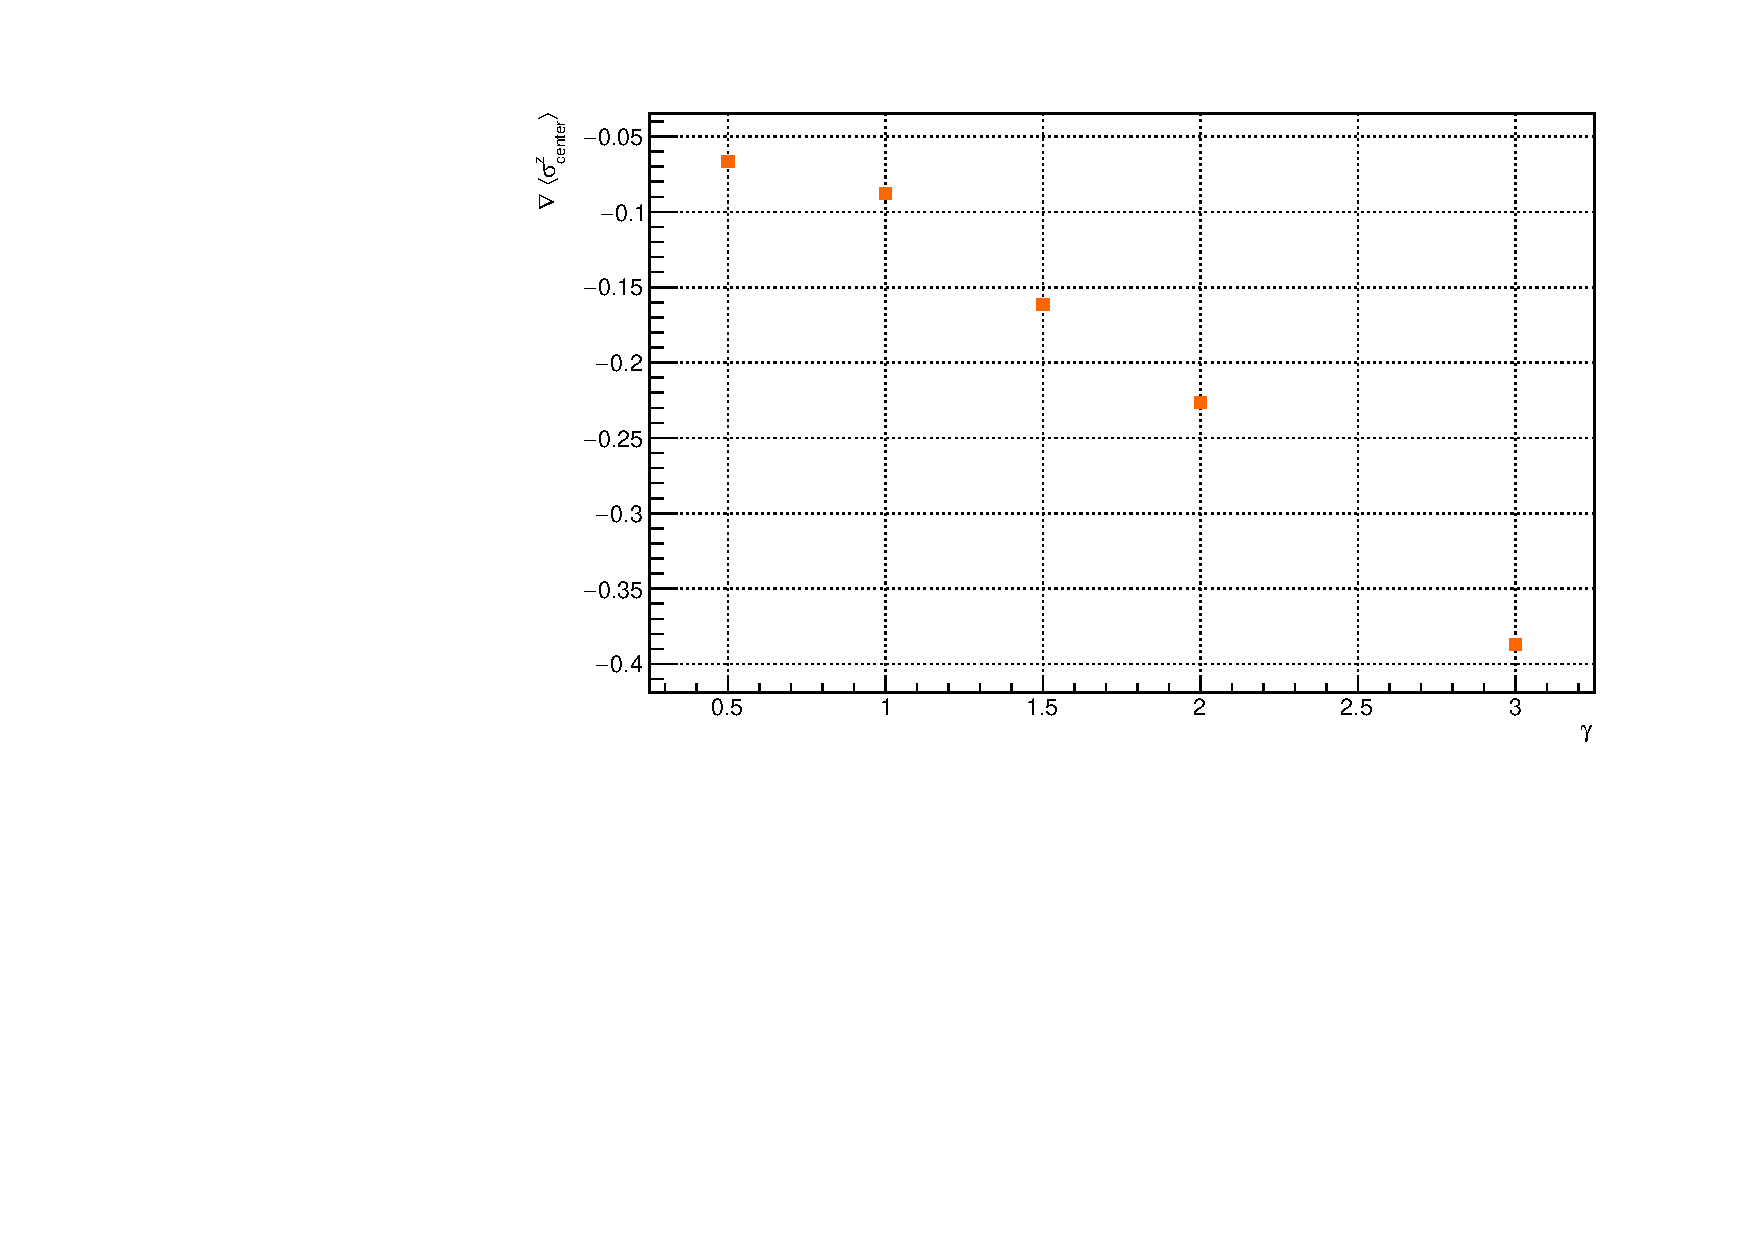
\includegraphics[scale=0.7]{Figures/12sites/12sites_gradLM_centerChainVSgamma.pdf}
    \caption{\textcolor{red}{FIT}}
    \label{fig:my_label}
\end{figure}

\begin{figure}[H]
    \centering
    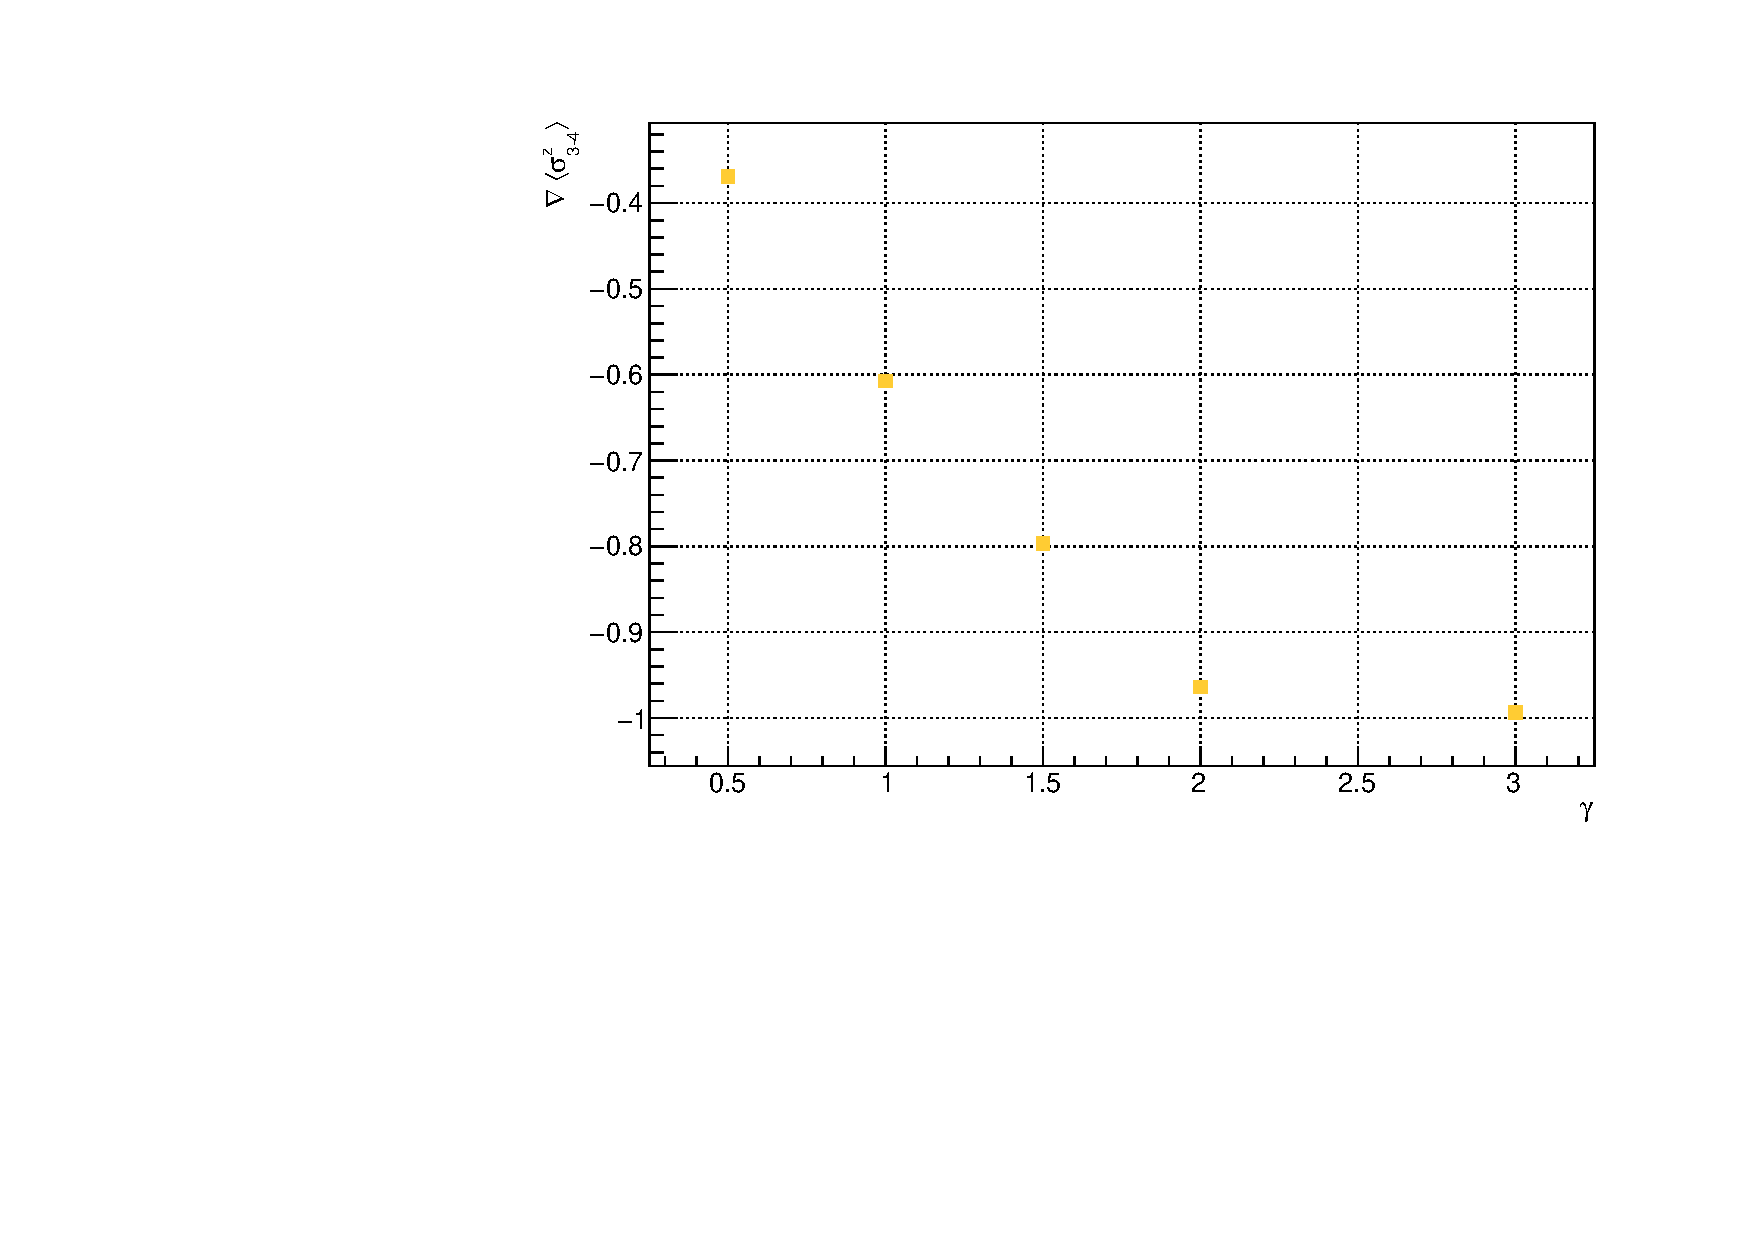
\includegraphics[scale=0.7]{Figures/12sites/12sites_gradLM_3and4VSgamma.pdf}
    \caption{\textcolor{red}{FIT}}
    \label{fig:my_label}
\end{figure}

\begin{figure}[H]
    \centering
    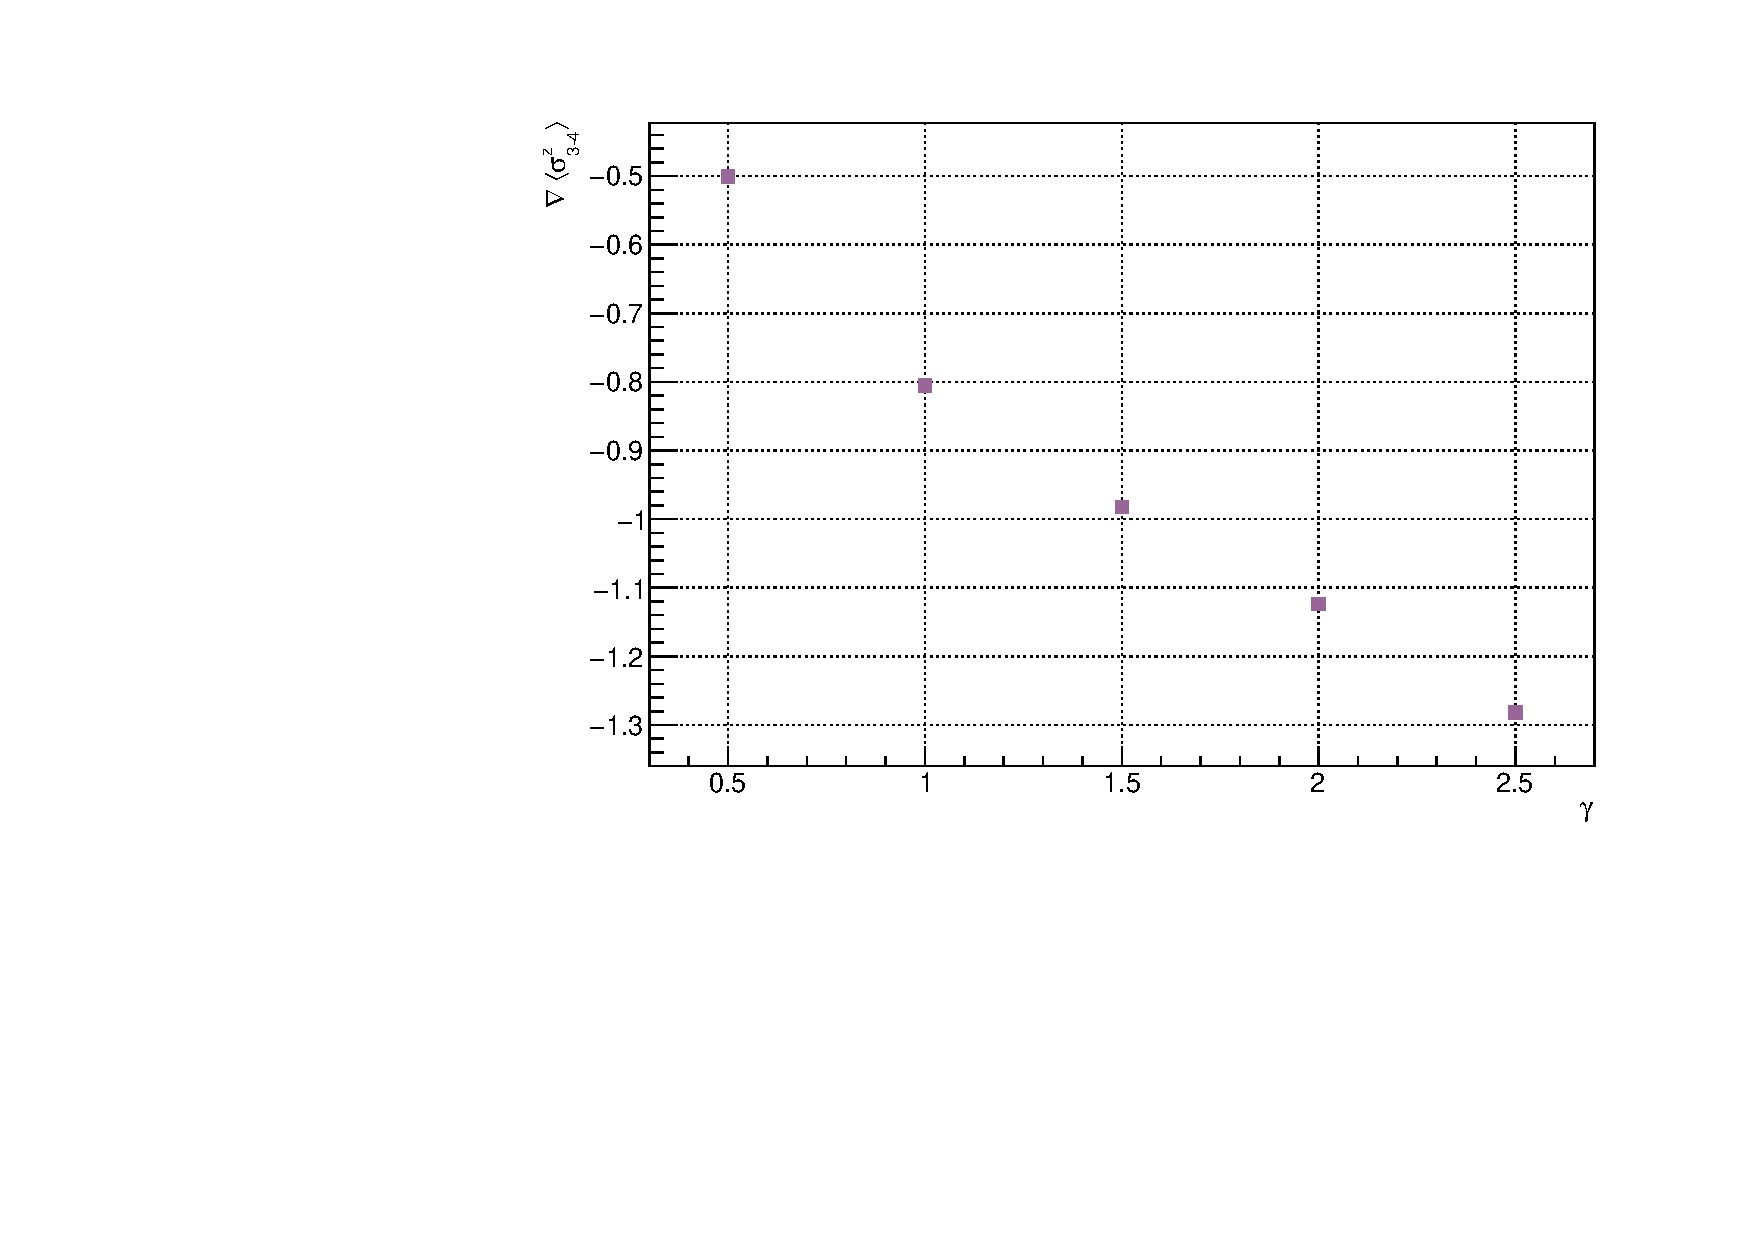
\includegraphics[scale=0.7]{Figures/16sites/16sites_gradLM_3and4VSgamma.pdf}
    \caption{\textcolor{red}{FIT}}
    \label{fig:my_label}
\end{figure}

\textcolor{red}{COMMENT}

\begin{figure}[H]
    \centering
    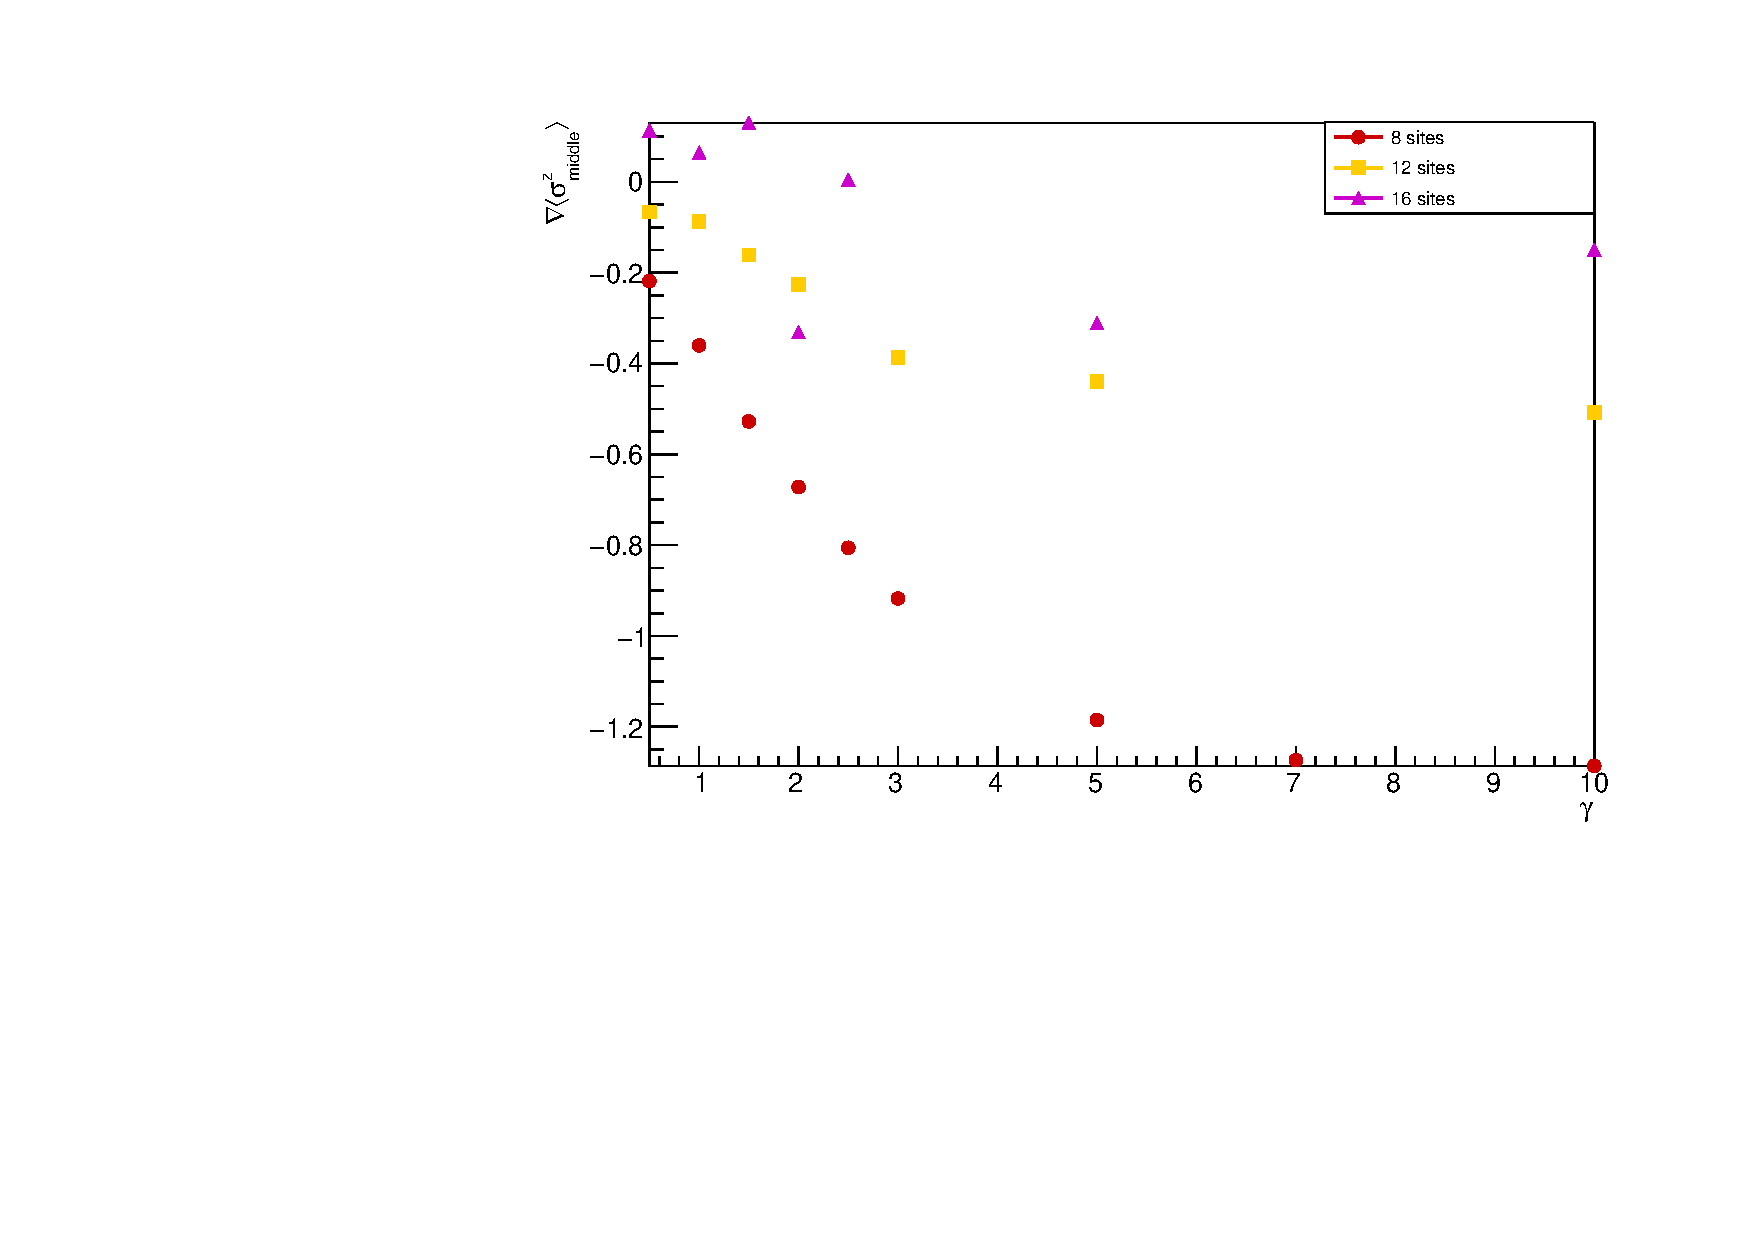
\includegraphics[scale=0.7]{Figures/gradLMvsGammavsSize.pdf}
    \caption{}
    \label{fig:my_label}
\end{figure}

\begin{figure}[H]
    \centering
    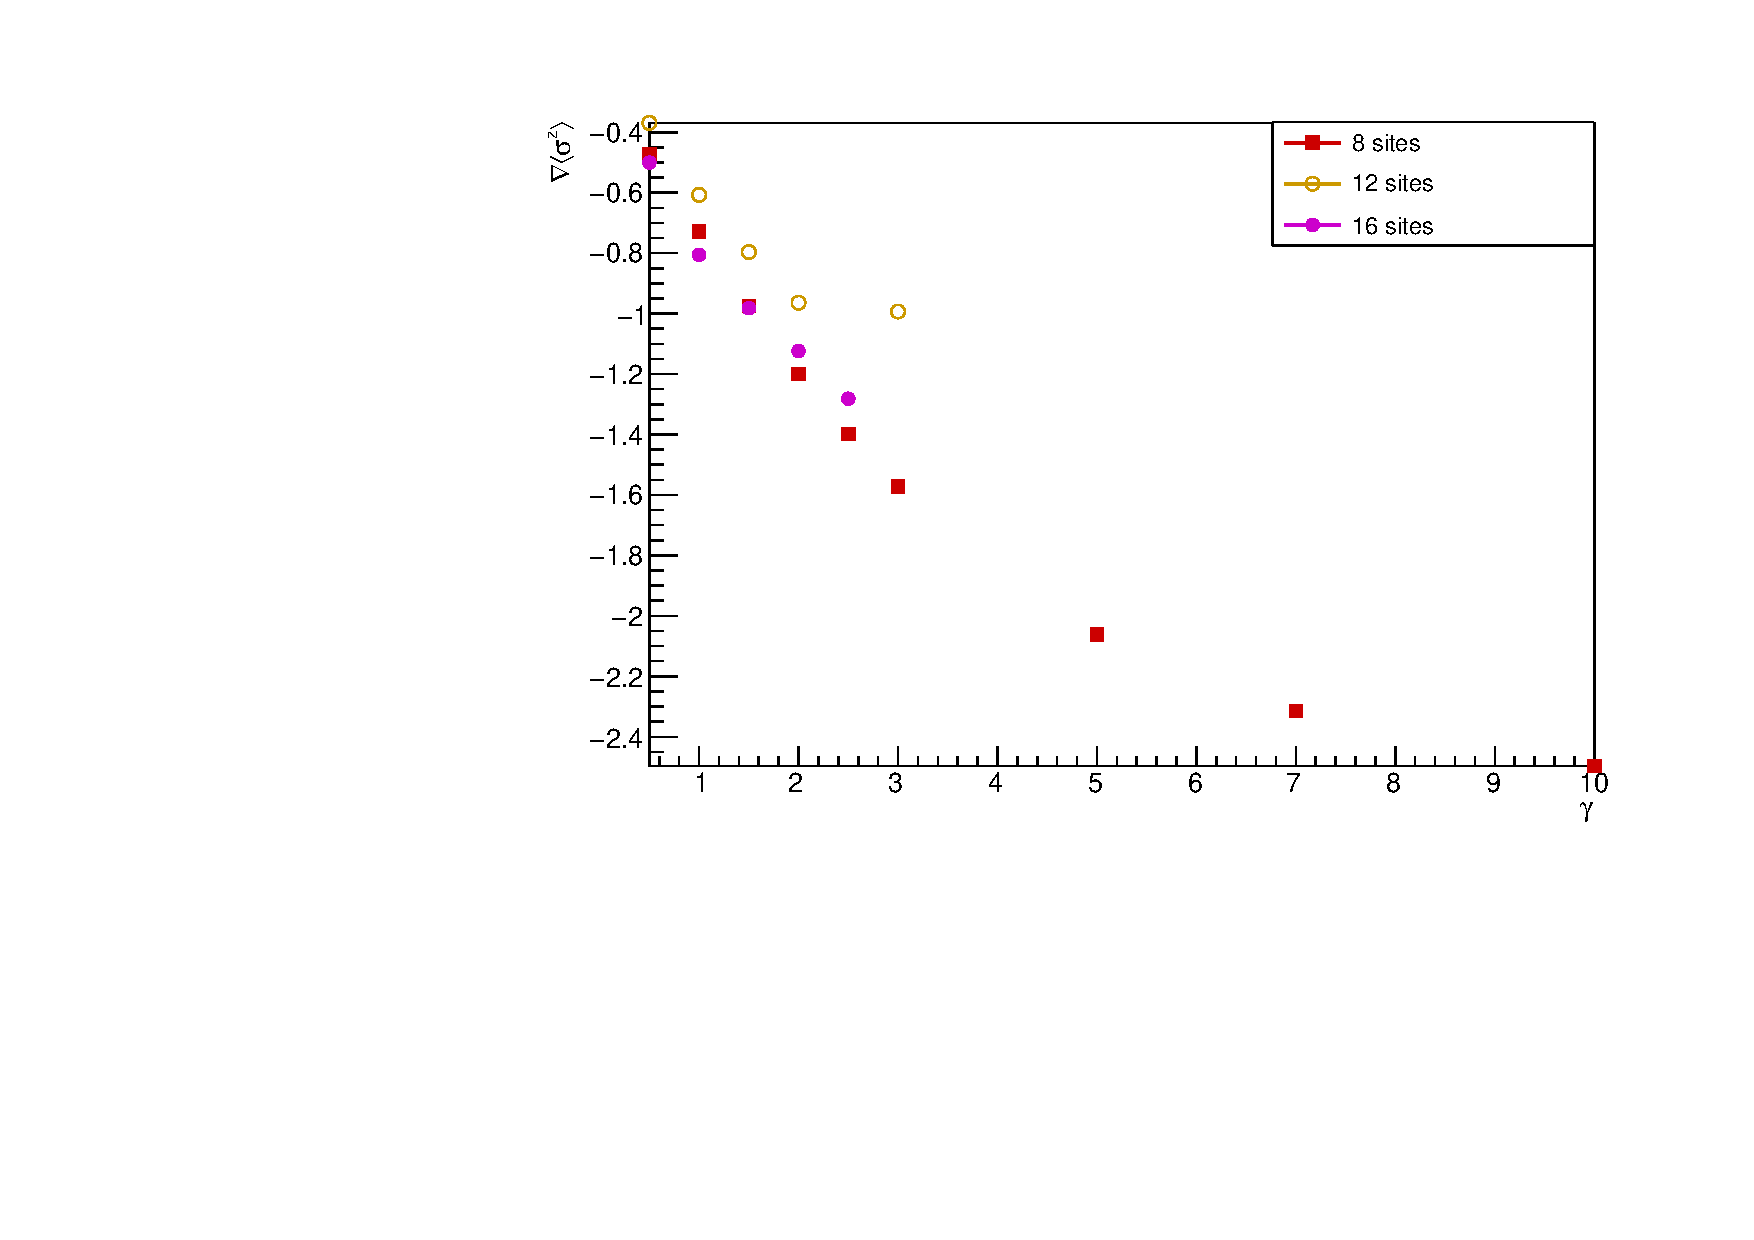
\includegraphics[scale=0.7]{Figures/gradLMvsGammavsSize_firstQuarterChain.pdf}
    \caption{}
    \label{fig:my_label}
\end{figure}

%%%%%%%%%%%%%%%%%%%%%%%%%%%%%%%%%%%%%%%%%%%%%%%%%%%%%%%%%%%%%%%%%%%%%%%%%%%%%%%%%%%%%%%%%%%%%%%%%%%%%%%%%%%%%%%%%%%%%%%%%%%%%%%%%%%%%%%%%%%%%%%%%%%%%%%%%%%%%%%%%%%%%%%%%%%%%%%%%%%%%%%%%%%%%%%%%%%%%%%%%%%%%%%%%%%%%%%%%%%%%%%%%%%%%%%%%%%%%%%%%%%%%%%%%%%%%%%%%%%%%
\section{Two-Points Correlation Functions}
Another observable of interest is certainly the steady-state two-point correlation function, defined as follows:
\begin{equation}
    C(i, j) = \langle \sigma^z_i \sigma^z_j \rangle - \langle \sigma^z_i \rangle \langle \sigma^z_j \rangle,
\end{equation}
where $\langle \sigma^z_i \sigma^z_j \rangle = \Tr(\sigma^z_i \sigma^z_j \rho_{s})$ and $\langle \sigma^z_i \rangle = \Tr(\sigma^z_i \rho_{s})$, being $\rho_{s}$ the steady-state density matrix.

First of all, as done in the last section, a comparison of the data obtained from MPO and QT method is shown; in particular, the spin-spin correlation function in relation to the first site $C(1, j)$ is displayed. In the following, the two-point correlation function will be studied considering the system symmetry, using the so-called \emph{bulk} correlation function; that is, starting from the middle sites of the chain, the correlation function will be calculated between equidistant sites from the center of the chain. 

\textcolor{red}{ATTENTION. THESE THREE PLOTS ARE JUST <SIGMASIGMA> WITHOUT THE CONNECTION TERM. TODO}
\begin{figure}[H]
    \centering
    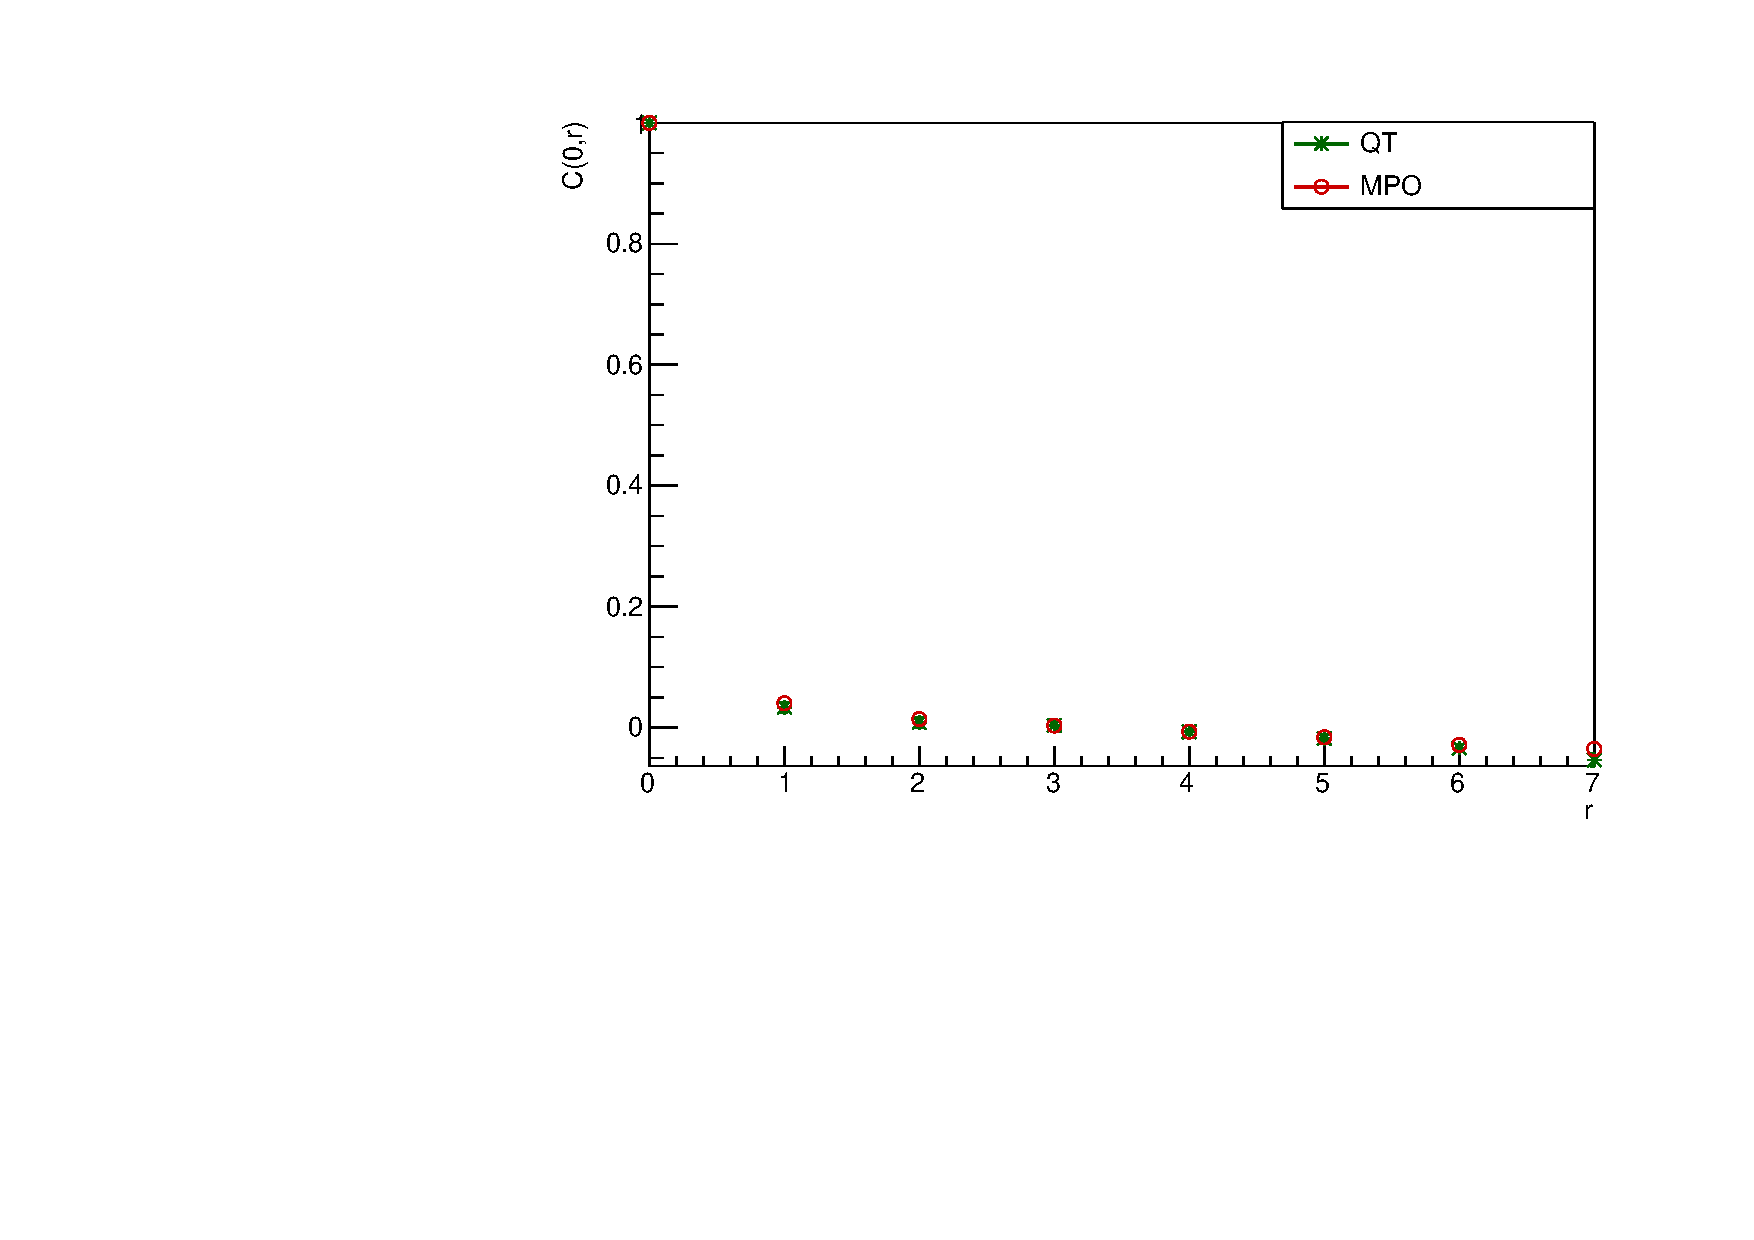
\includegraphics[scale=0.7]{Figures/8sites/CorrFunc1_8s_J10505.pdf}
    \caption{Correlation function with respect to the spin positioned in the first site of the chain, characterized by $\gamma~=~1, J_x=1, J_y=0.5, J_z=0.5$; \emph{i} stands for the site index.}
    \label{fig:my_label}
\end{figure}

\begin{figure}[H]
    \centering
    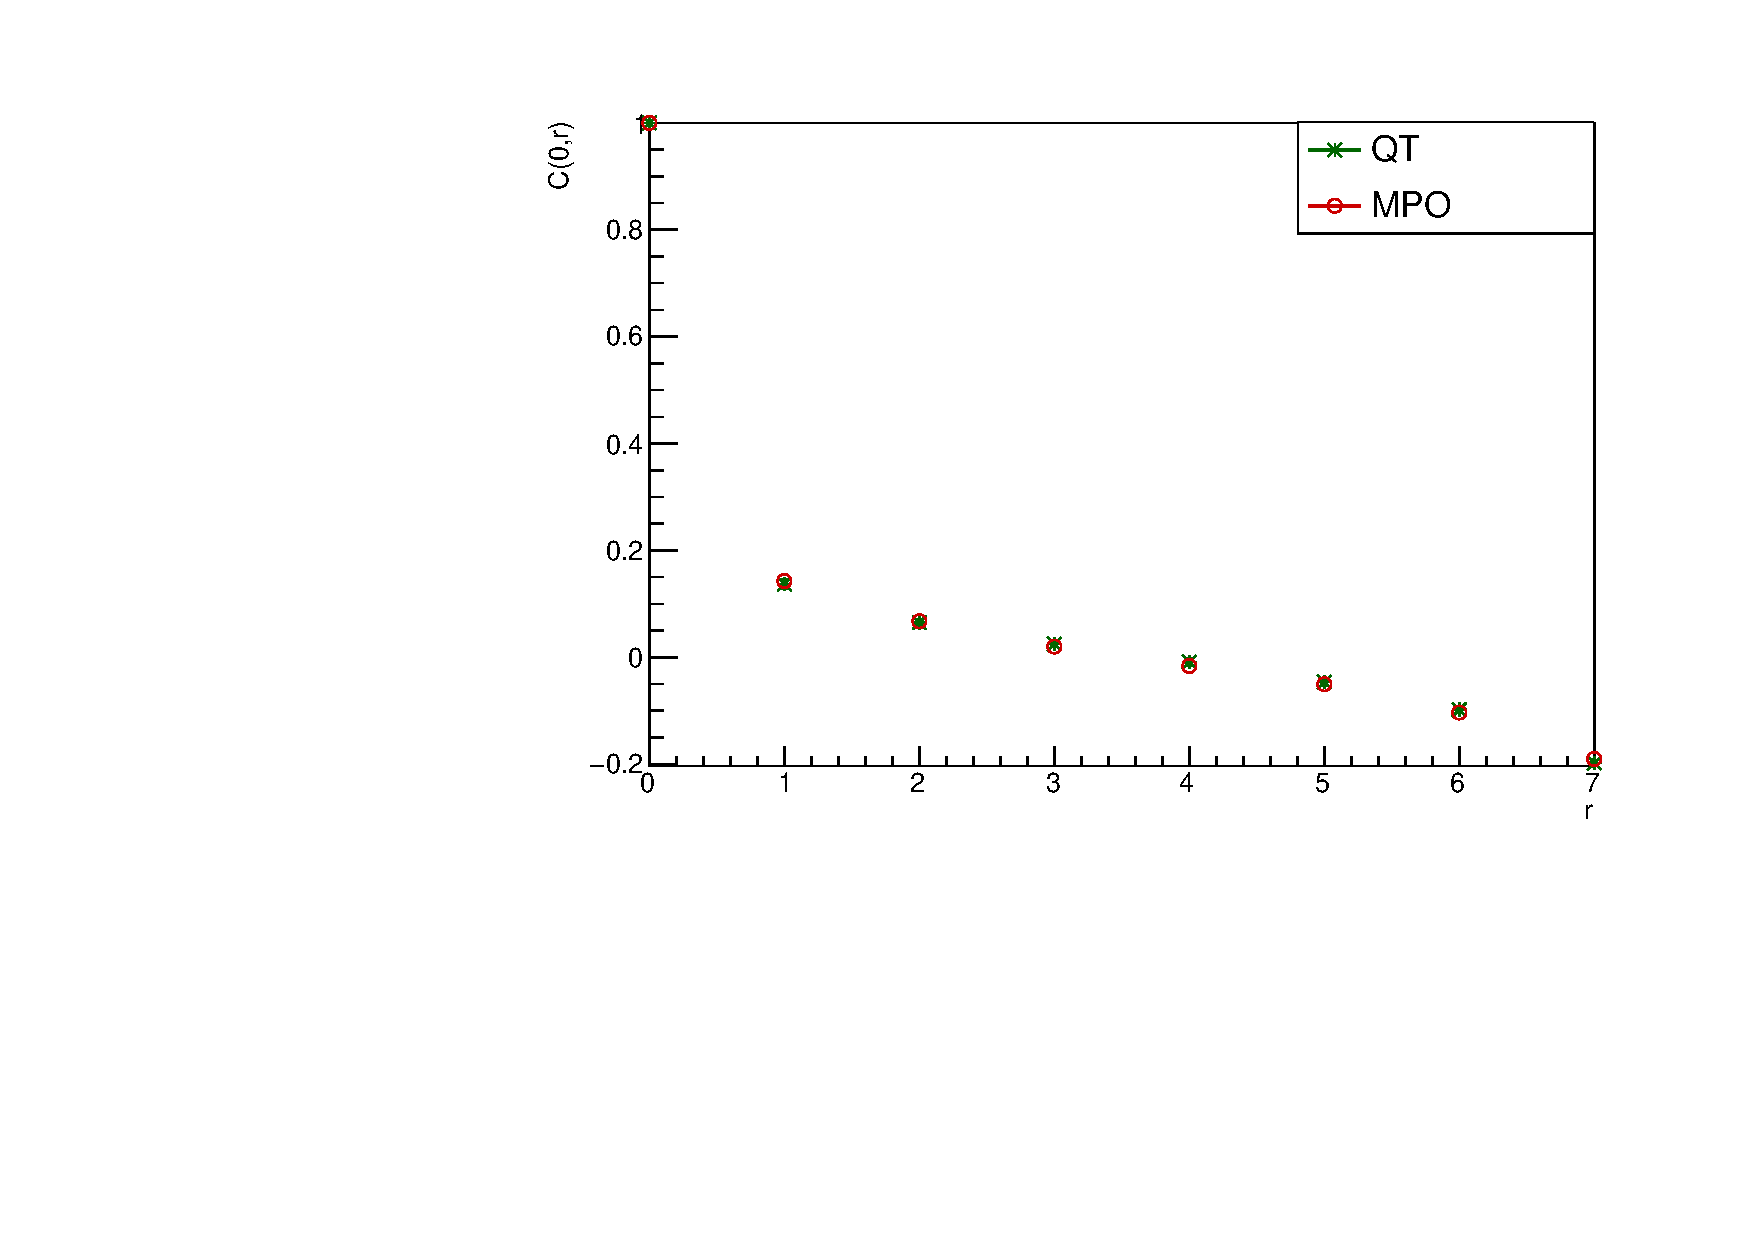
\includegraphics[scale=0.7]{Figures/8sites/CorrFunc1_8s_J1051.pdf}
    \caption{Correlation function with respect to the spin positioned in the first site of the chain, characterized by $\gamma~=~1, J_x=1, J_y=0.5, J_z=1$; \emph{i} stands for the site index.}
    \label{fig:my_label}
\end{figure}

\begin{figure}[H]
    \centering
    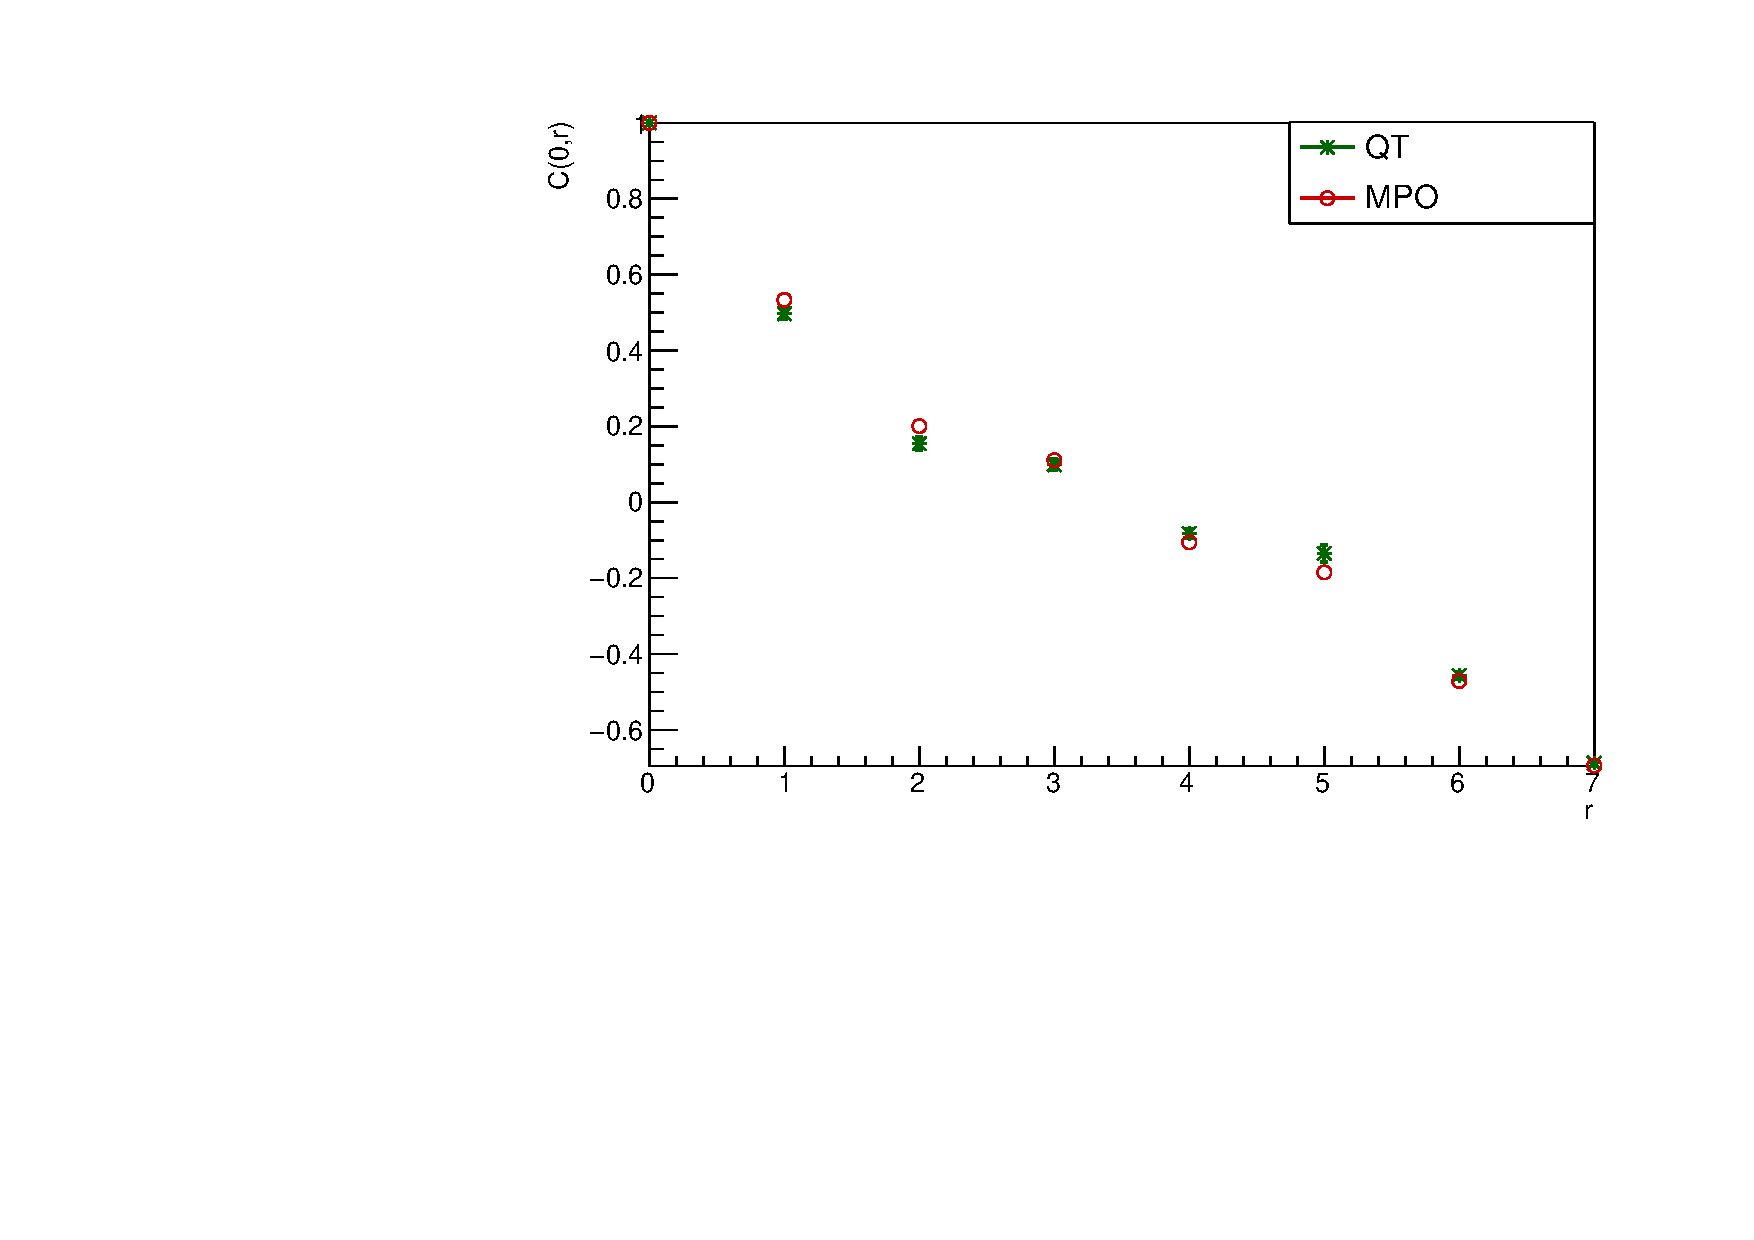
\includegraphics[scale=0.7]{Figures/8sites/CorrFunc1_8s_J10515.pdf}
    \caption{Correlation function with respect to the spin positioned in the first site of the chain, characterized by $\gamma~=~1, J_x=1, J_y=0.5, J_z=1.5$; \emph{i} stands for the site index.}
    \label{fig:my_label}
\end{figure}

The same is done for the bulk correlation function, calculated as explained previously.

\begin{figure}[H]
    \centering
    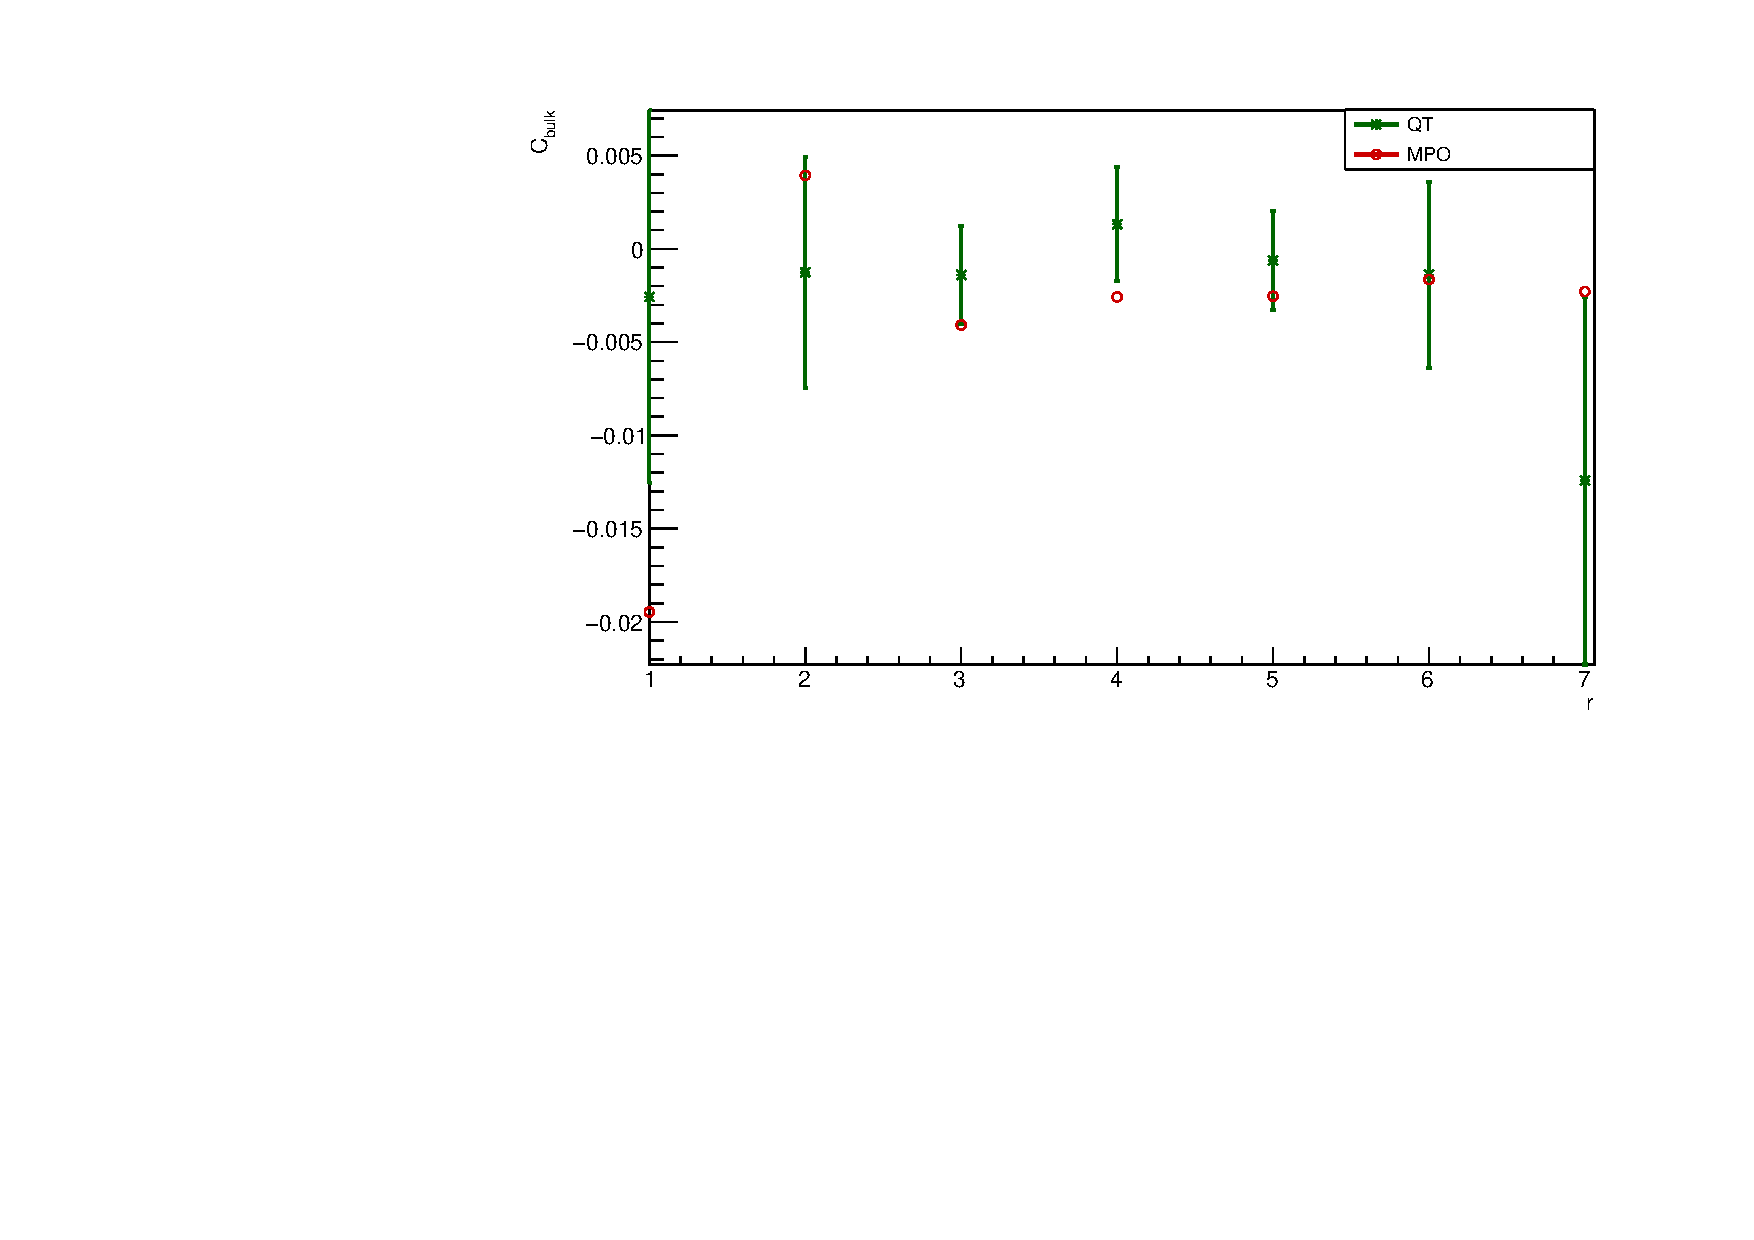
\includegraphics[scale=0.7]{Figures/8sites/CorrFuncBulkCONN_8sJ10505.pdf}
    \caption{Bulk correlation function for a 8-sites chain characterized by $\gamma~=~1, J_x=1, J_y=0.5, J_z=0.5$.}
    \label{fig:my_label}
\end{figure}

\begin{figure}[H]
    \centering
    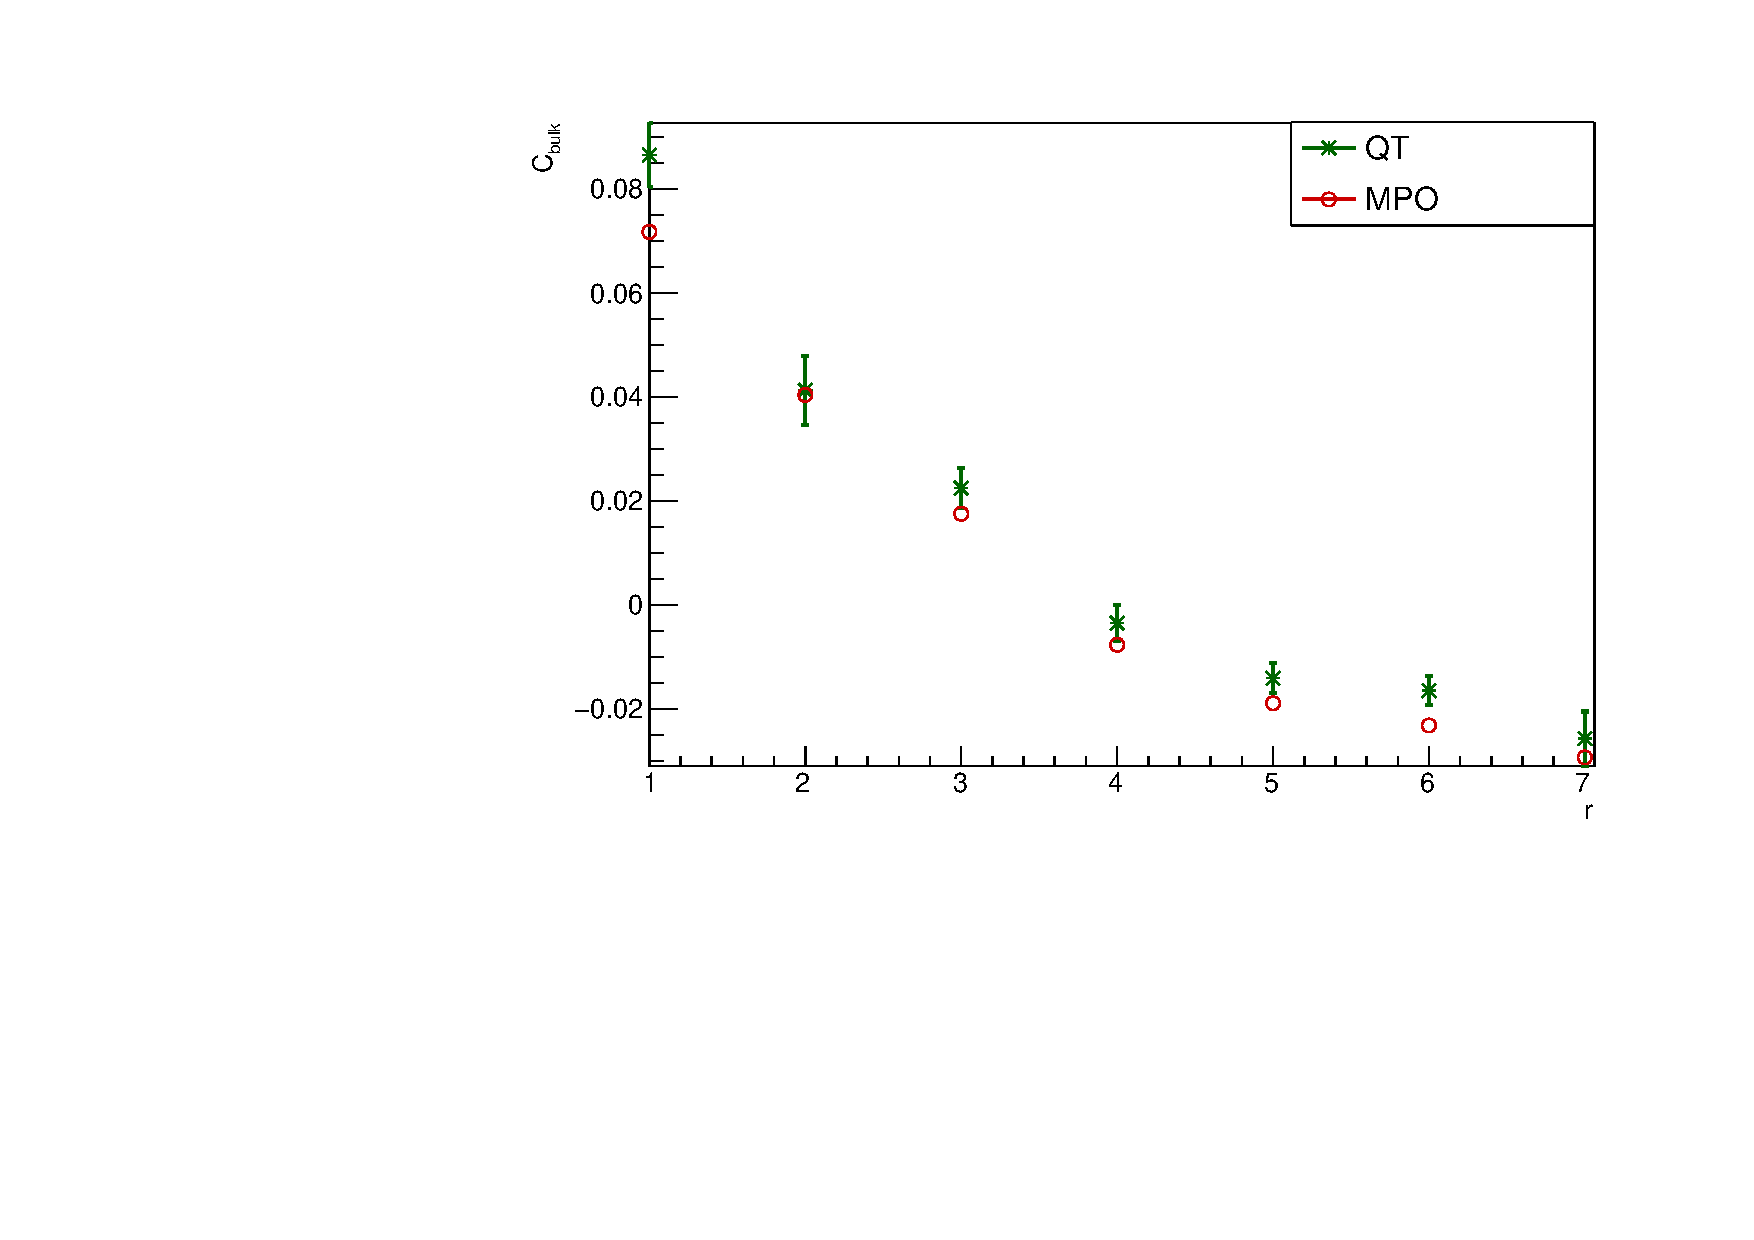
\includegraphics[scale=0.7]{Figures/8sites/CorrFuncBulkCONN_8sJ1051.pdf}
    \caption{Bulk correlation function for a 8-sites chain characterized by $\gamma~=~1, J_x=1, J_y=0.5, J_z=1$.}
    \label{fig:my_label}
\end{figure}

\begin{figure}[H]
    \centering
    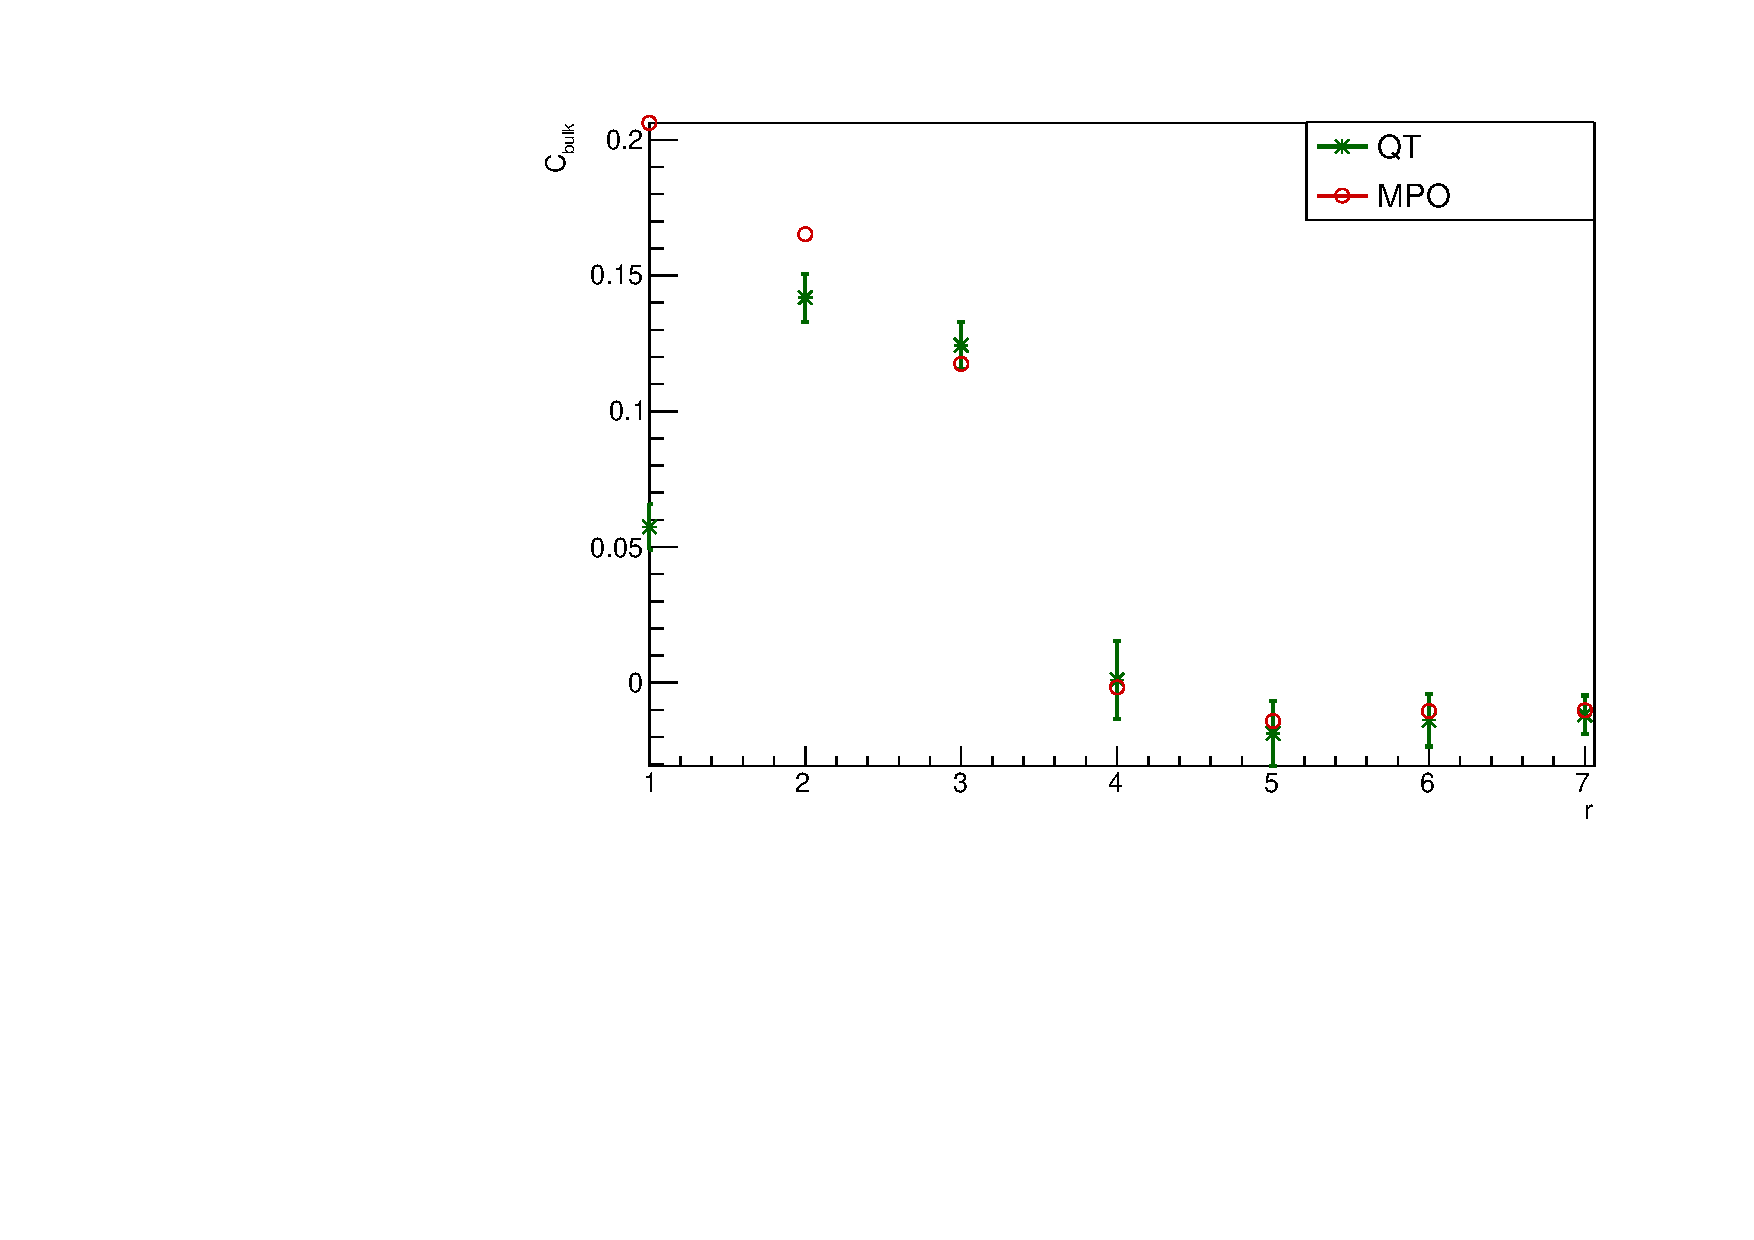
\includegraphics[scale=0.7]{Figures/8sites/CorrFuncBulkCONN_8sJ10515.pdf}
    \caption{Bulk correlation function for a 8-sites chain characterized by $\gamma~=~1, J_x=1, J_y=0.5, J_z=1.5$.}
    \label{fig:my_label}
\end{figure}

In the fig.~\ref{fig:8sites_CBulkConnVSgamma}, \ref{fig:12sites_CFBulkCONNVSgamma}, \ref{fig:16sites_CFBulkCONNVSgamma} the bulk correlation function for several values of $\gamma$ is shown, for 8, 12 and 16 sites spin chain respectively. An interesting aspect that is quite clear in these plots, involves the finite-size effect; while the size of the chain grows, the exponential profile of the correlation function become more clear. 

\begin{figure}[H]
    \centering
    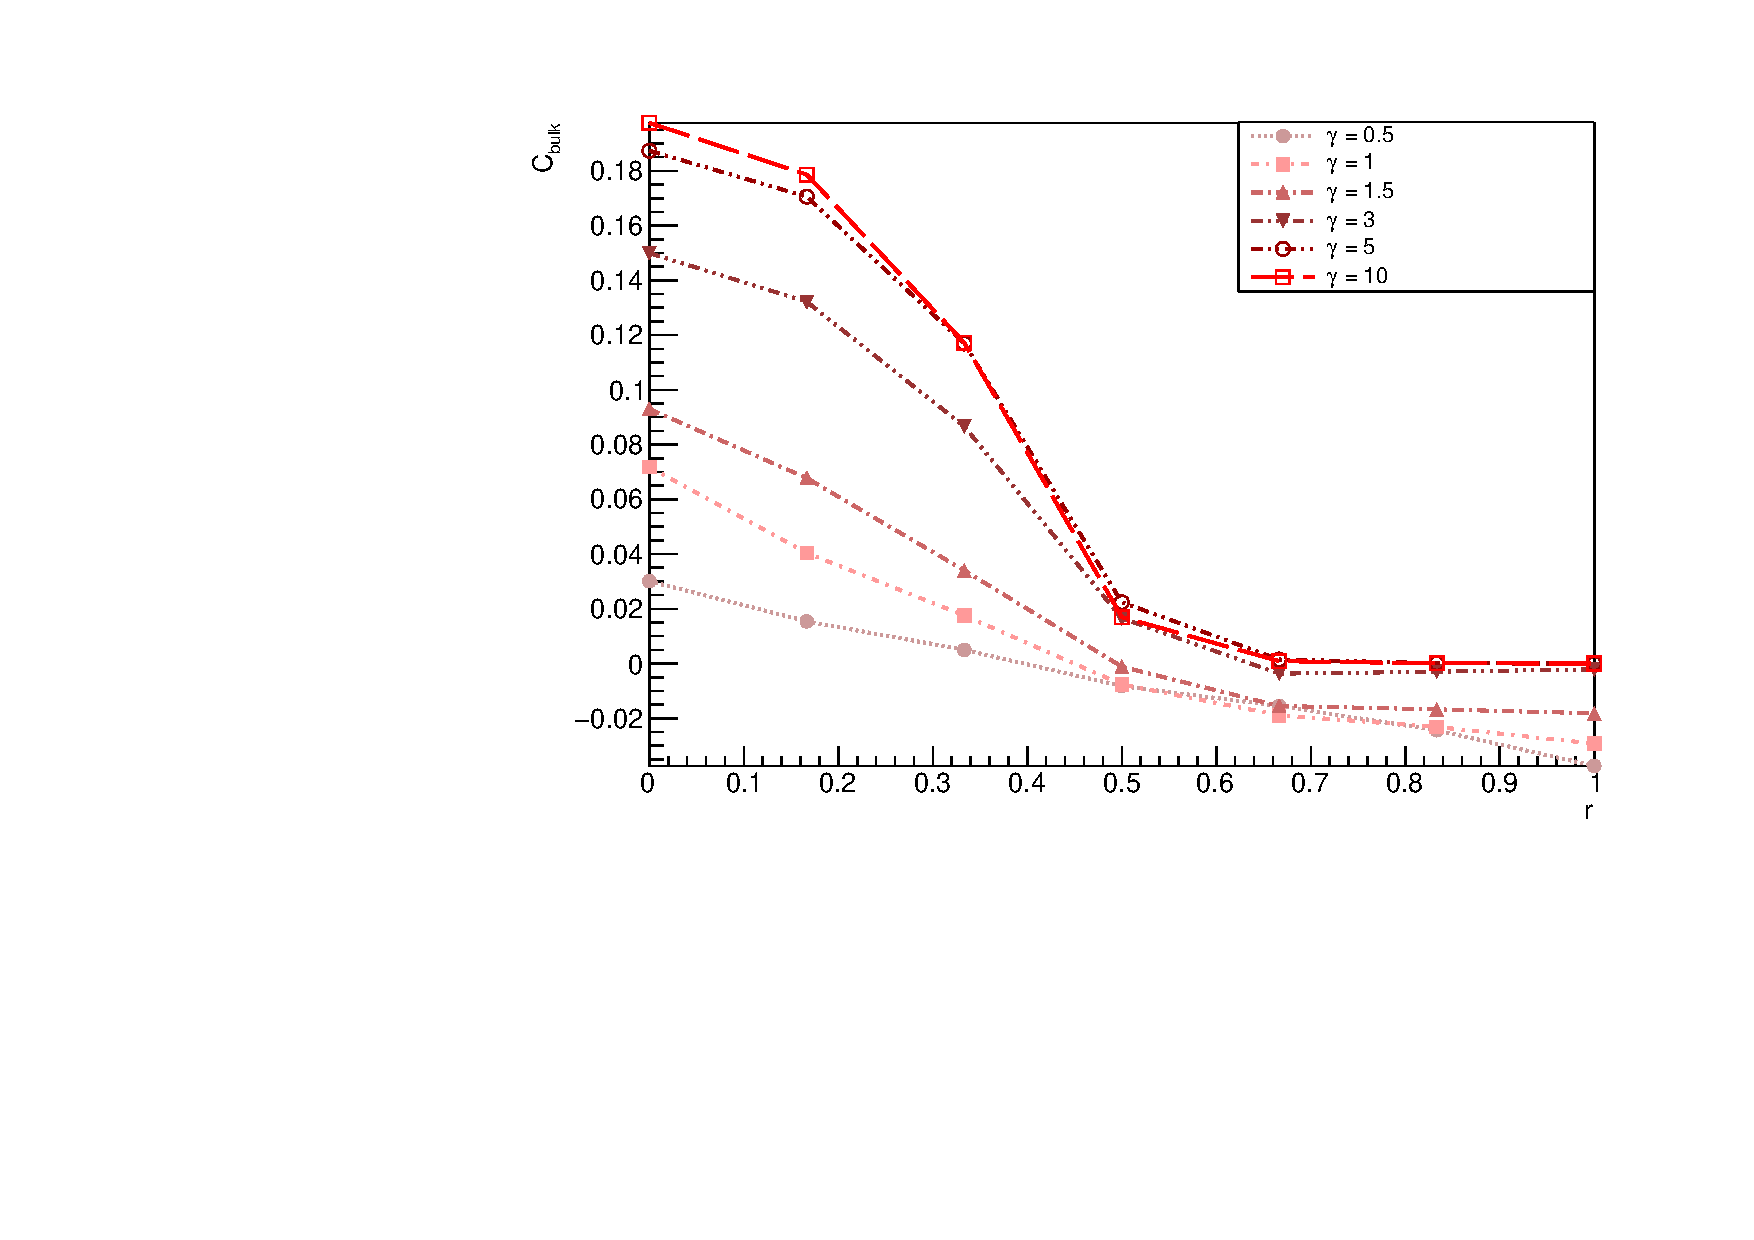
\includegraphics[scale=0.7]{Figures/8sites_CBulkConnVSgamma.pdf}
    \caption{Bulk correlation function for a 8-sites spin chain. Data are obtained from MPO method.}
    \label{fig:8sites_CBulkConnVSgamma}
\end{figure}

\begin{figure}[H]
    \centering
    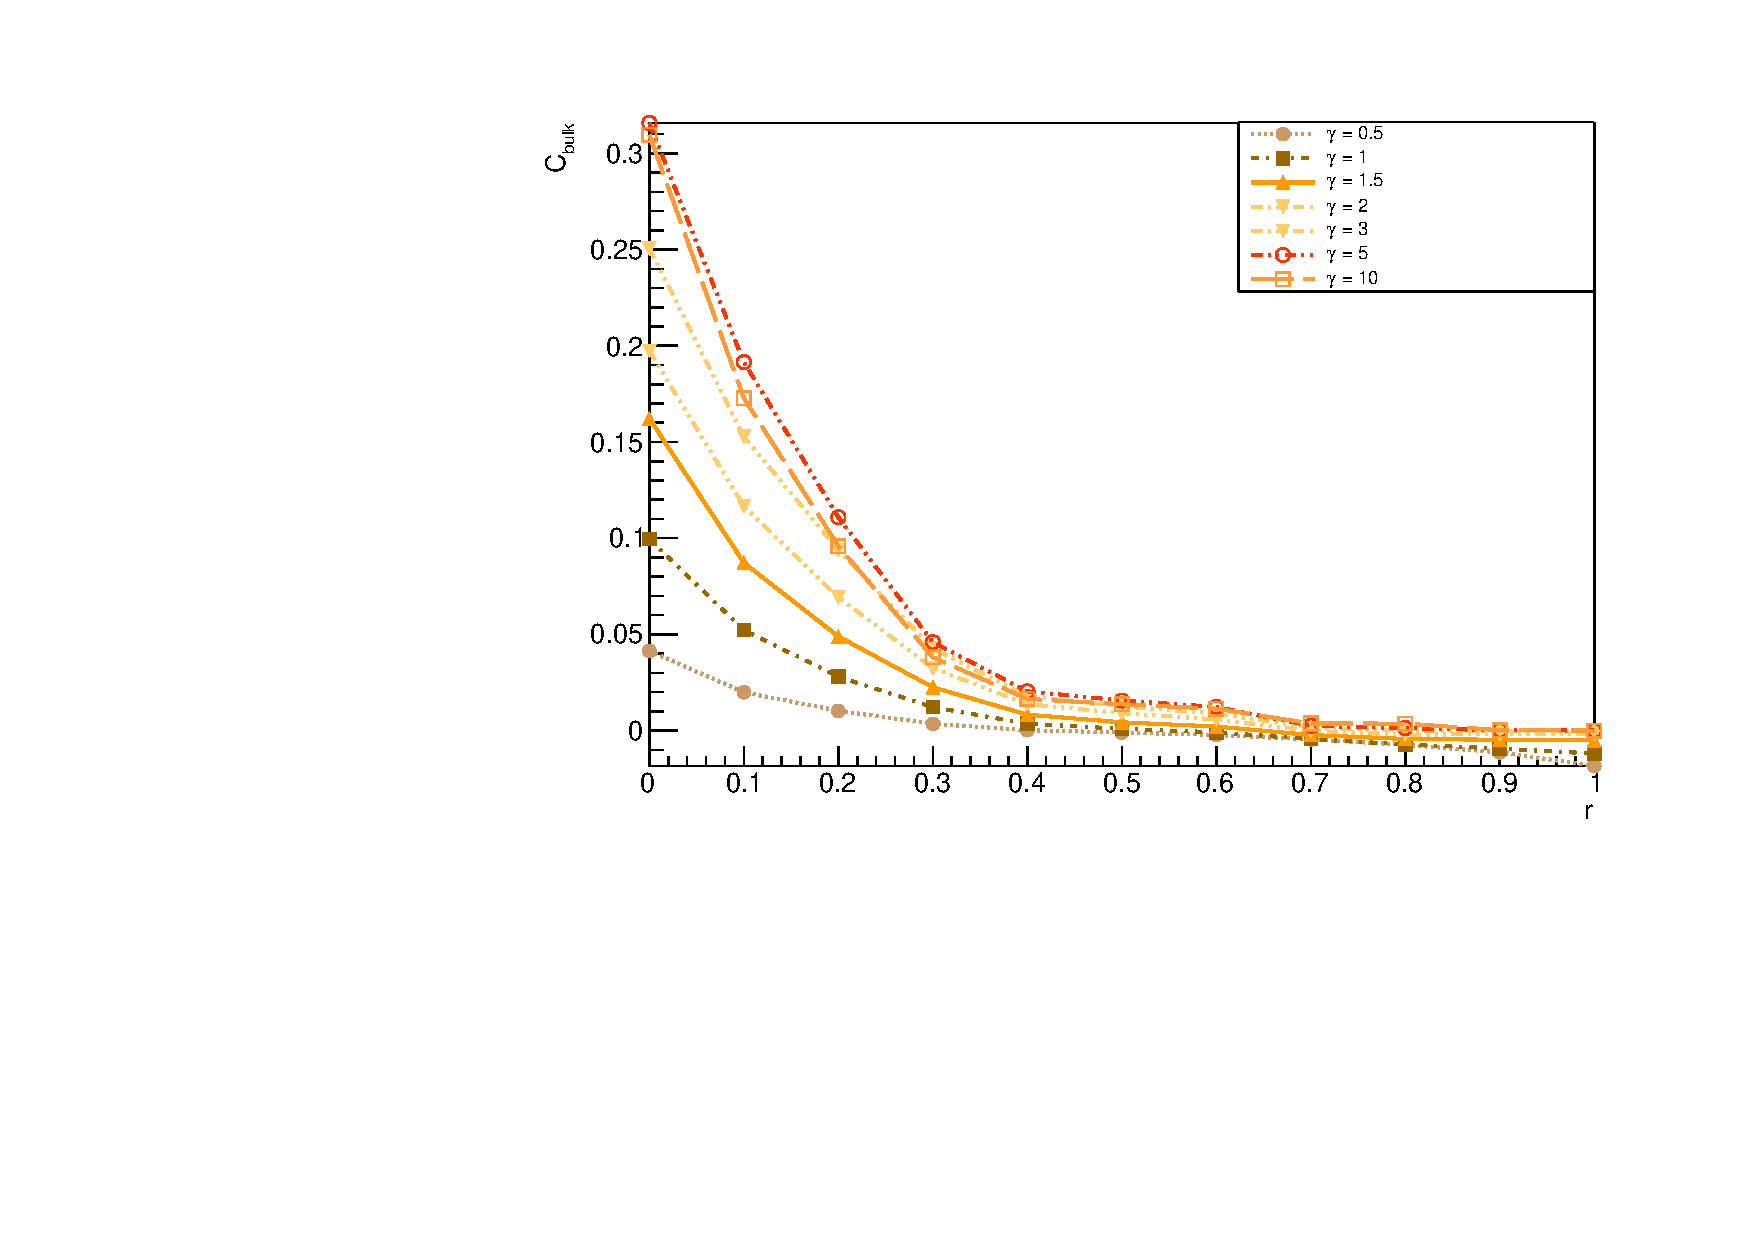
\includegraphics[scale=0.7]{Figures/12sites/12sites_CFBulkCONNVSgamma.pdf}
    \caption{Bulk correlation function for a 12-sites spin chain. Data are obtained from MPO method.}
    \label{fig:12sites_CFBulkCONNVSgamma}
\end{figure}

\begin{figure}[H]
    \centering
    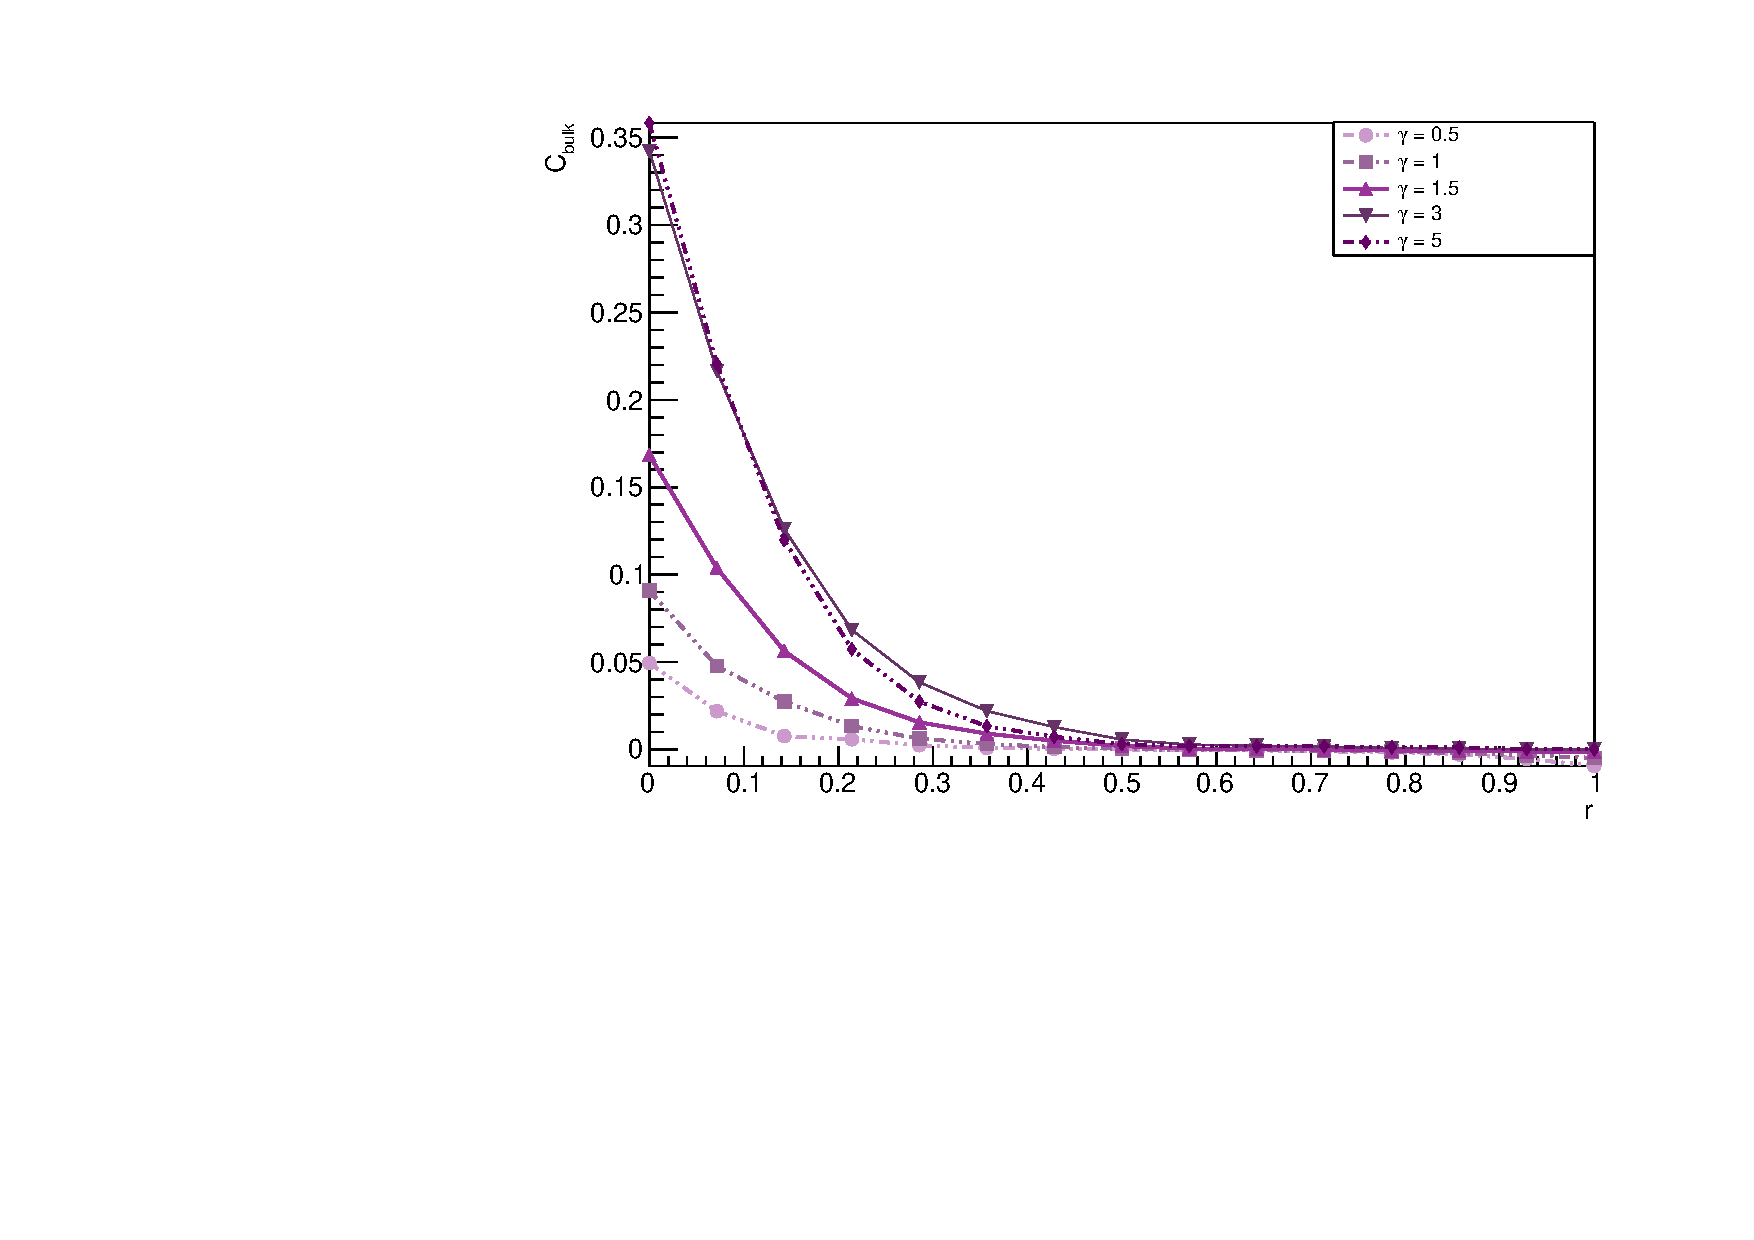
\includegraphics[scale=0.7]{Figures/16sites/16sites_CFBulkCONNVSgamma.pdf}
    \caption{Bulk correlation function for a 16-sites spin chain. Data are obtained from MPO method. \textcolor{red}{TODO: FIT}}
    \label{fig:16sites_CFBulkCONNVSgamma}
\end{figure}

Let us see how the bulk correlation function changes varying in the chain size.

\begin{figure}[H]
    \centering
    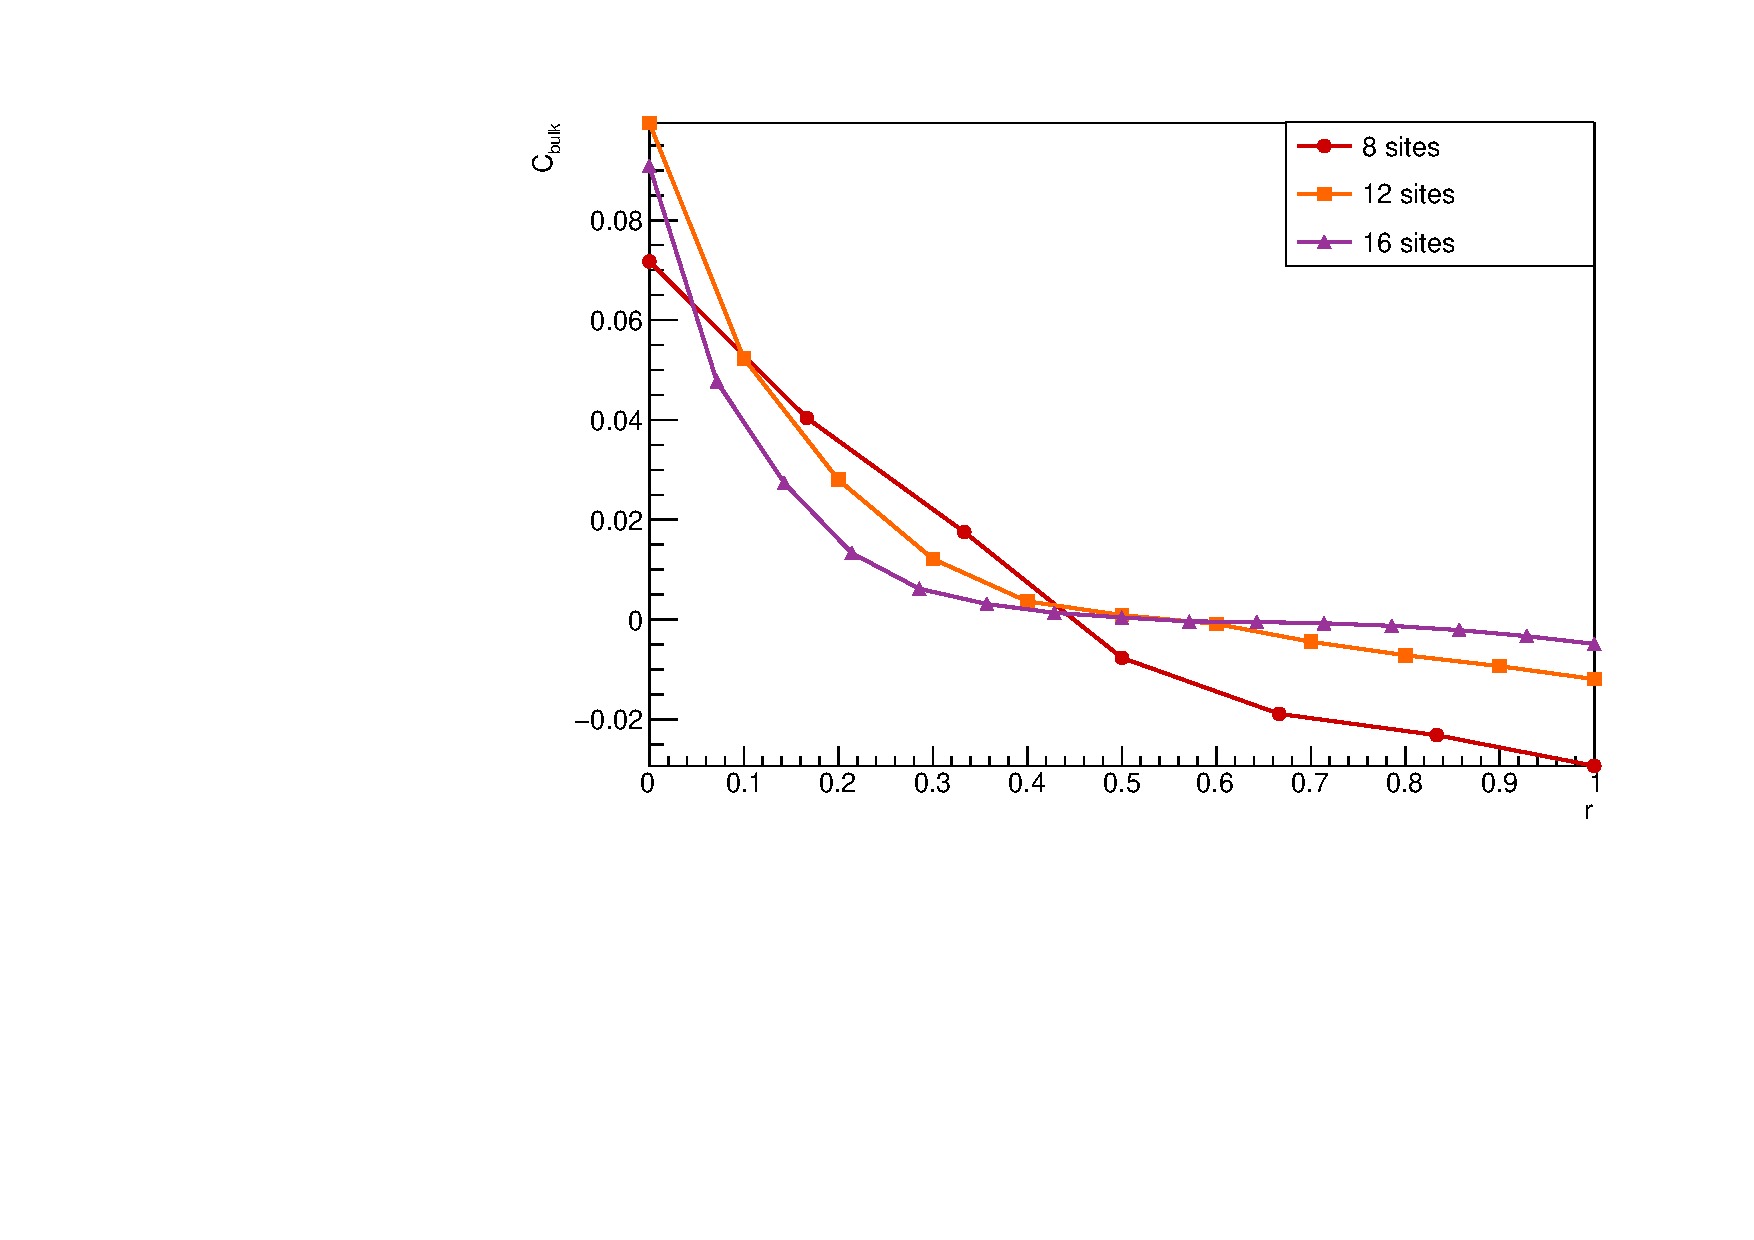
\includegraphics[scale=0.7]{Figures/CBulkwConnTermVSsize_J1051.pdf}
    \caption{Comparison between bulk correlation function for a 8, 12, 16 sites spin chain, with $J_z = 1$ and $\gamma = 1$. Data are obtained from MPO method.}
    \label{fig:CBulkwConnTermVSsize_J1051}
\end{figure}

%%%%%%%%%%%%%%%%%%%%%%%%%%%%%%%%%%%%%%%%%%%%%%%%%%%%%%%%%%%%%%%%%%%%%%%%%%%%%%%%%%%%%%%%%%%%%%%%%%%%%%%%%%%%%%%%%%%%%%%%%%%%%%%%%%%%%%%%%%%%%%%%%%%%%%%%%%%%%%%%%%%%%%%%%%%%%%%%%%%%%%%%%%%%%%%%%%%%%%%%%%%%%%%%%%%%%%%%%%%%%%%%%%%%%%%%%%%%%%%%%%%%%%%%%%%%%%%%%%
\section{Spin Transport}
In this section we are going to study the spin current $j_\sigma$ defined from the continuity equation for the local spin operators~\cite{BenentiCasatiProsenRossini}:
\begin{equation}
    \frac{\partial S^k_z}{\partial t} + \nabla (j_\sigma)_k = 0,
\end{equation}
which can be rewritten as
\begin{equation}
    (j_\sigma)_{k+1}-(j_\sigma)_k = \frac{i}{2}[\sigma_k^z , H],
\end{equation}
where $S_k^z \equiv \sigma_k^z/2$ and where $H$ is the Hamiltonian written in~\ref{ham_chain}. So, we obtain:
\begin{equation}
    j_\sigma = J_y (\sigma_k^x \sigma_{k+1}^y) - J_x (\sigma_k^y \sigma_{k+1}^x). 
\end{equation}


\begin{figure}[H]
    \centering
    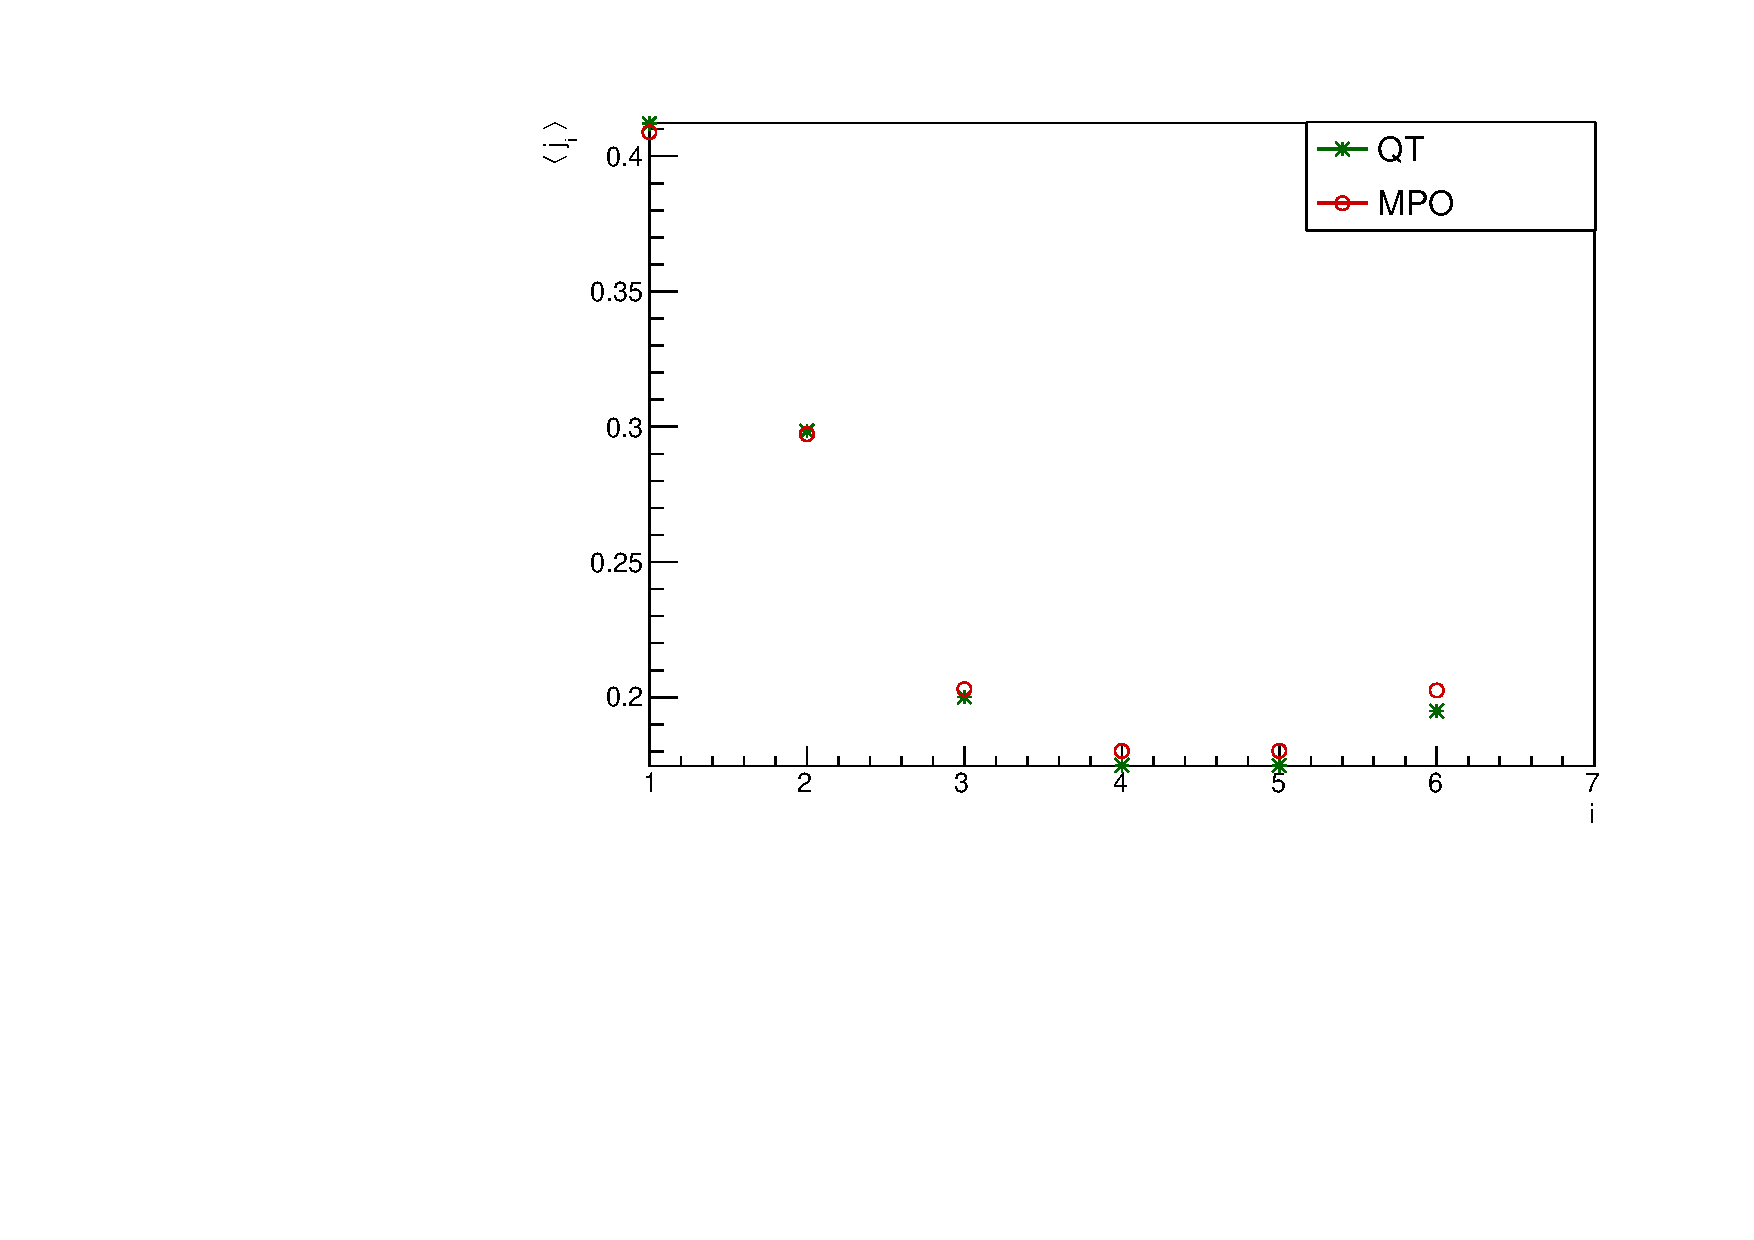
\includegraphics[scale=0.7]{Figures/8sites/SpinCurr_8s_J10505.pdf}
    \caption{Spin current of the chain, characterized by $\gamma=1, J_x=1, J_y=0.5, J_z=0.5$; \emph{i} stands for the site index.\textcolor{red}{DA RIVEDERE ERRORE}}
    \label{fig:my_label}
\end{figure}

\begin{figure}[H]
    \centering
    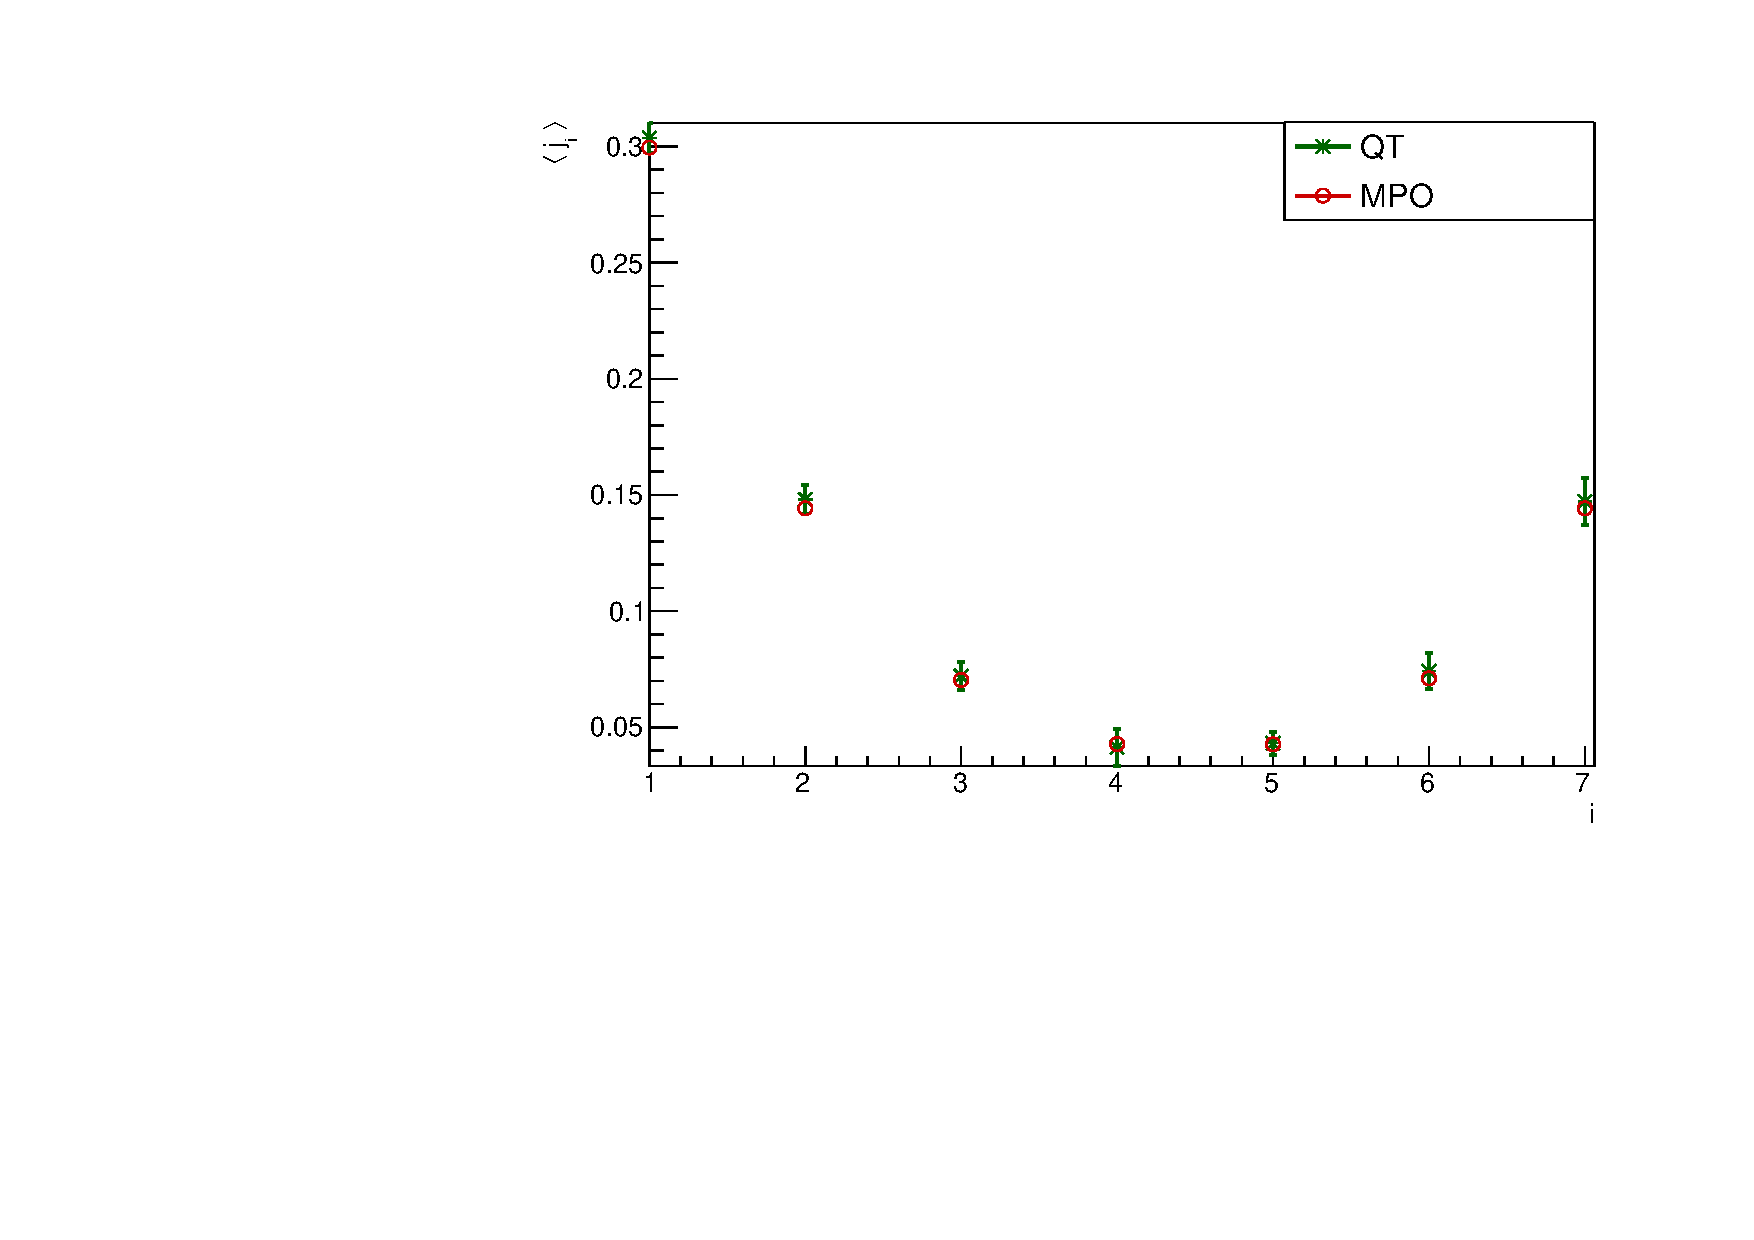
\includegraphics[scale=0.7]{Figures/8sites/SpinCurr_8s_J1051.pdf}
    \caption{Spin current of the chain, characterized by $\gamma=1, J_x=1, J_y=0.5, J_z=1$; \emph{i} stands for the site index.}
    \label{fig:my_label}
\end{figure}

\begin{figure}[H]
    \centering
    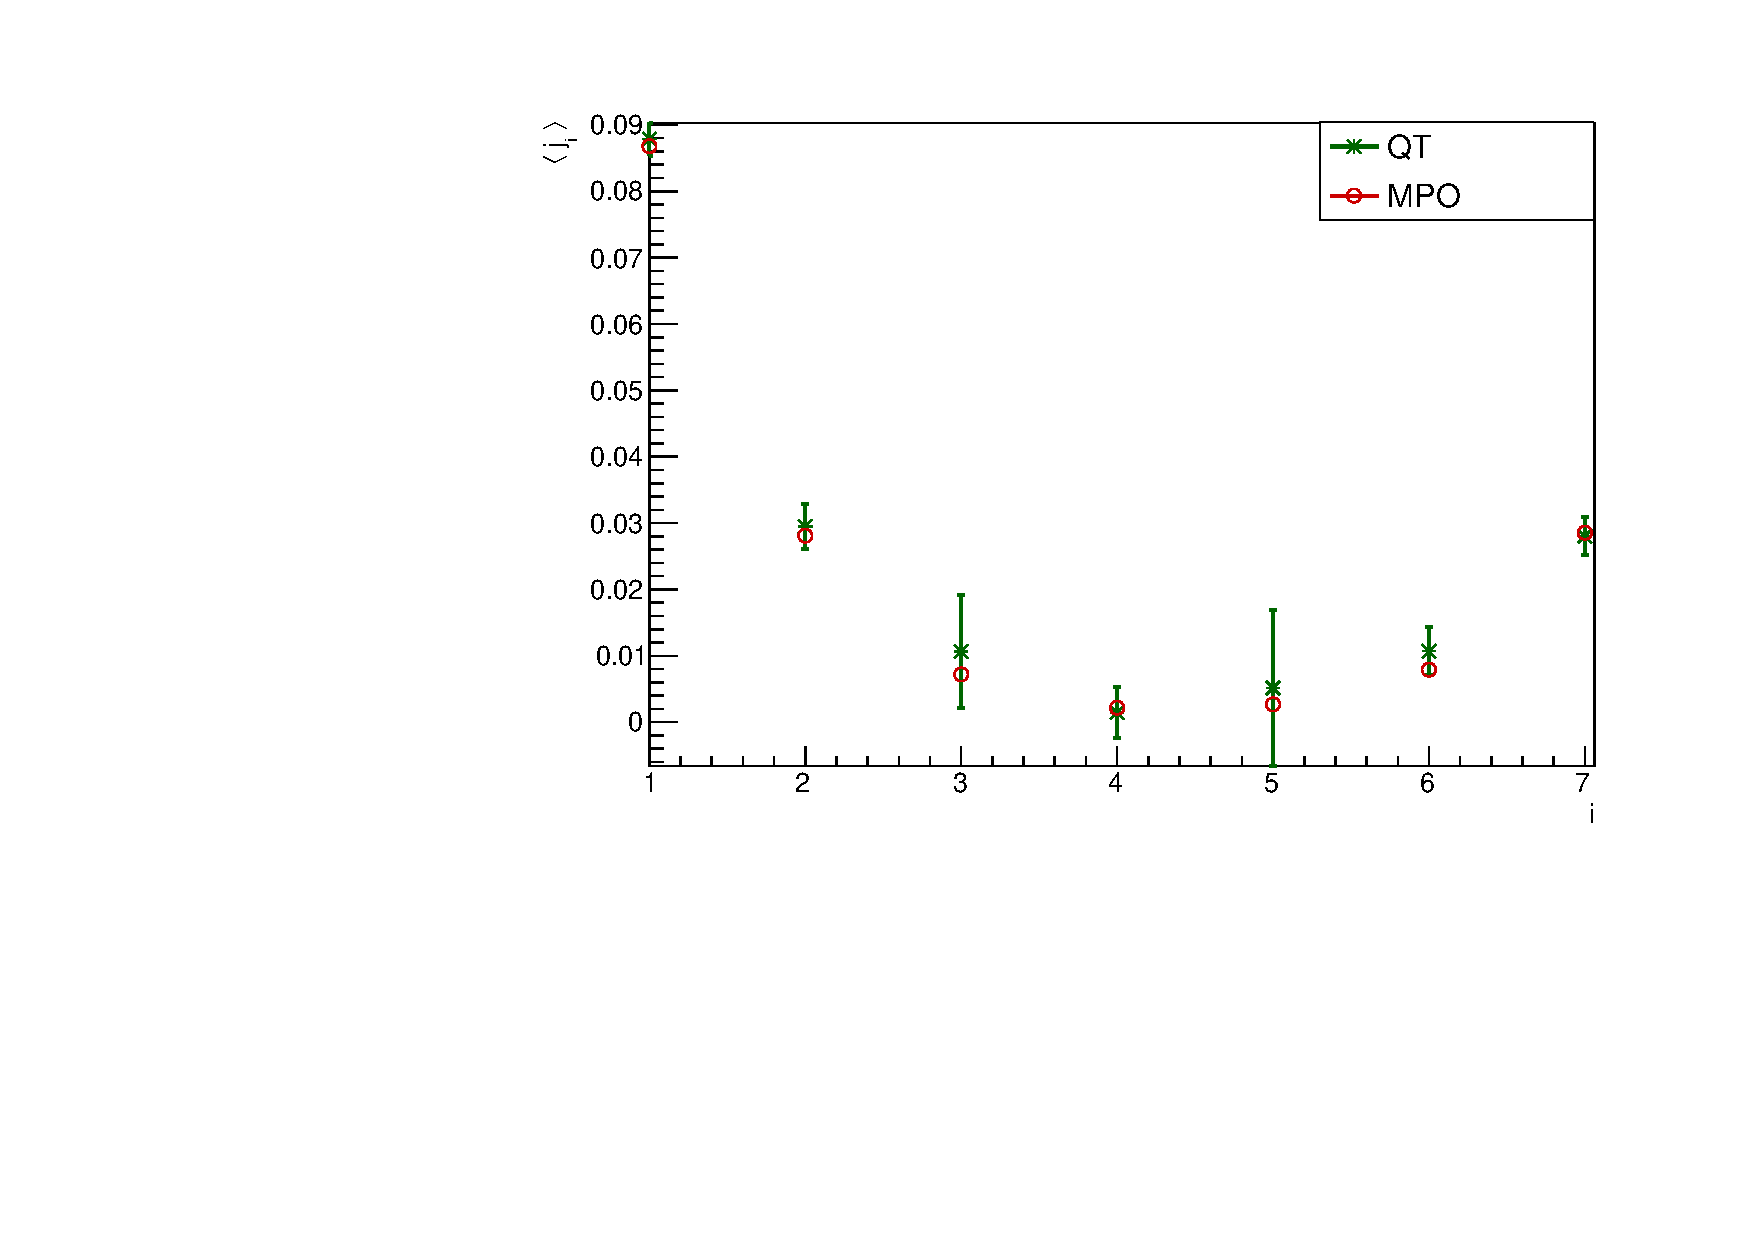
\includegraphics[scale=0.7]{Figures/8sites/SpinCurr_8s_J10515.pdf}
    \caption{Spin current of the chain, characterized by $\gamma=1, J_x=1, J_y=0.5, J_z=1.5$; \emph{i} stands for the site index.}
    \label{fig:my_label}
\end{figure}

%Let us see what happens in the case of a \textbf{12-sites} chain.
%
%\begin{figure}[H]
%    \centering
%    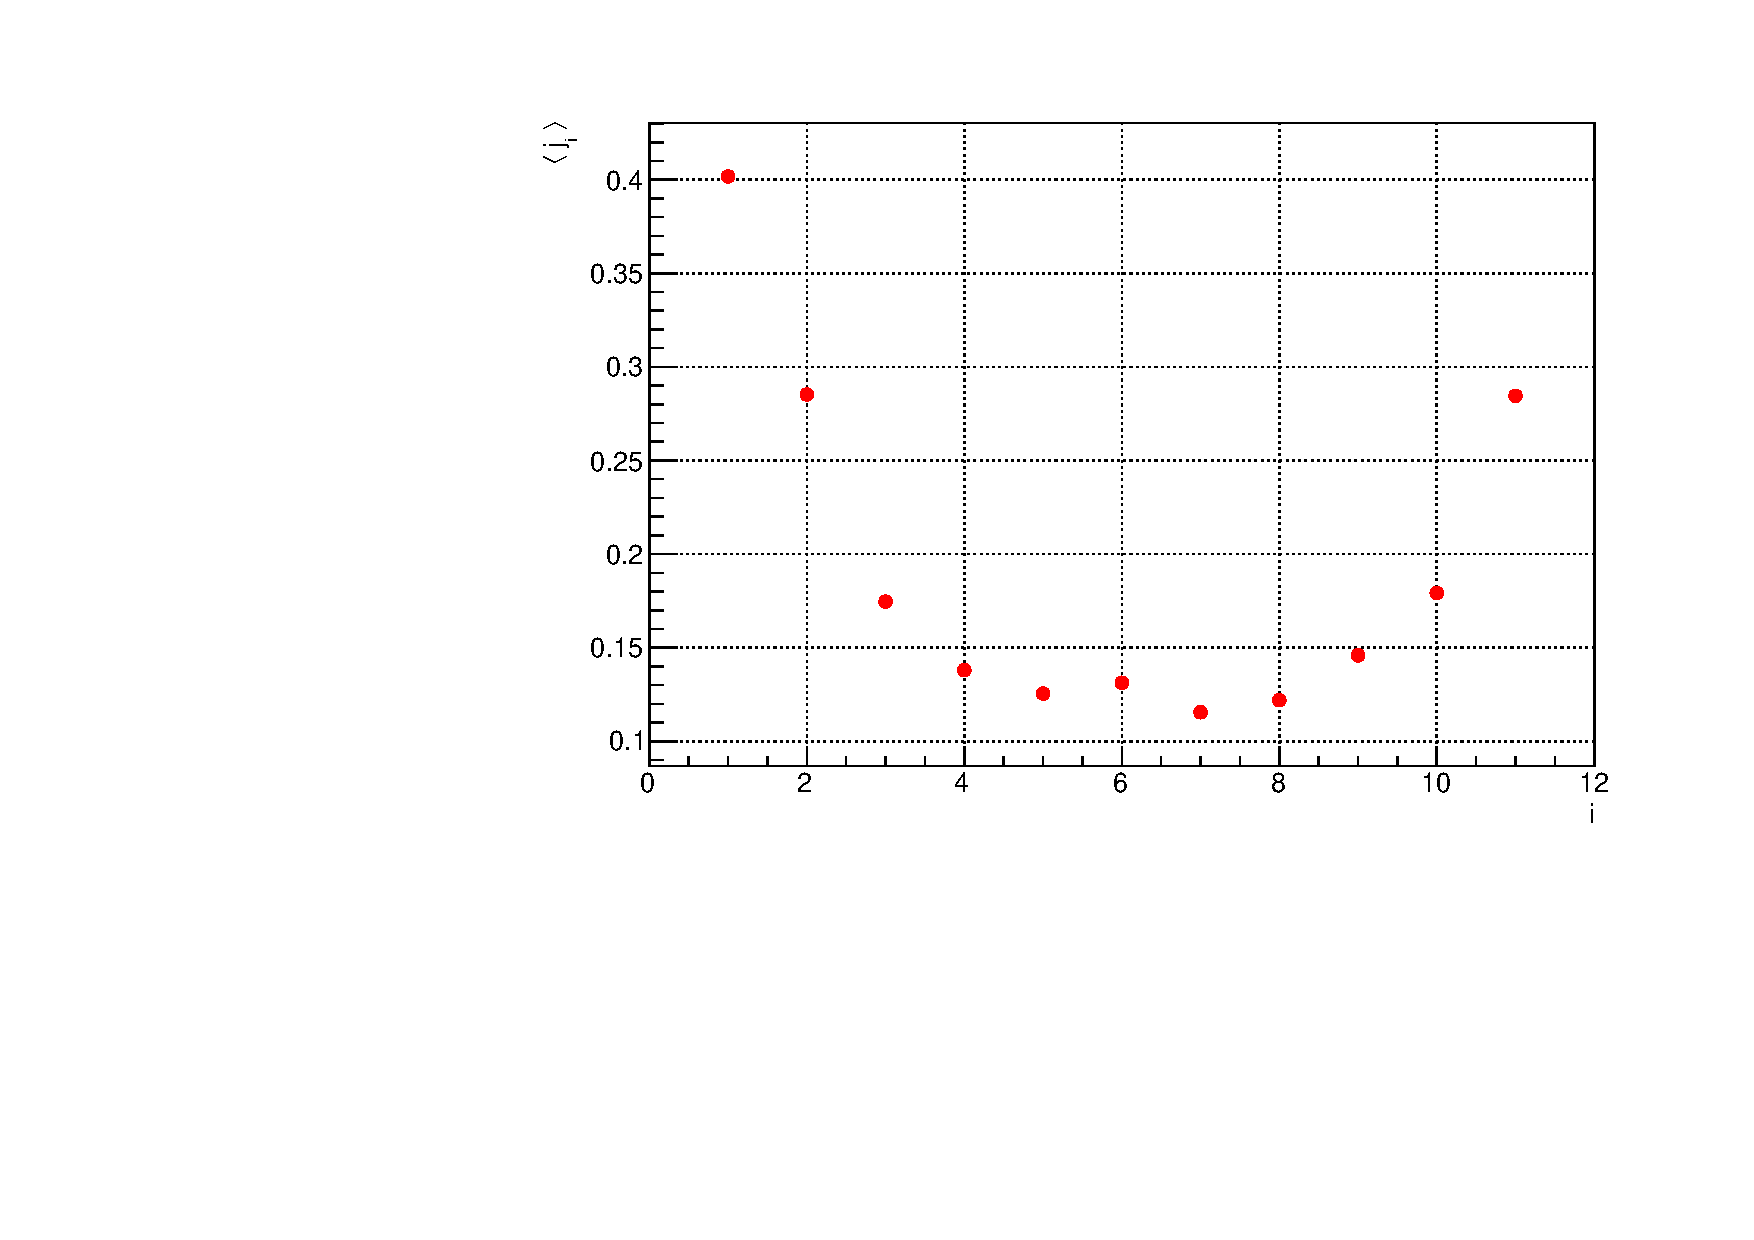
\includegraphics[scale=0.7]{Figures/12sites/SpinCurrL012m060Time002000_J10505.pdf}
%    \caption{Spin current of a 12-sites chain, characterized by $\gamma=1, J_x=1, J_y=0.5, J_z=0.5$; %\emph{i} stands for the site index. Data are obtained from MPO method.}
%    \label{fig:my_label}
%\end{figure}
%
%\begin{figure}[H]
%    \centering
%    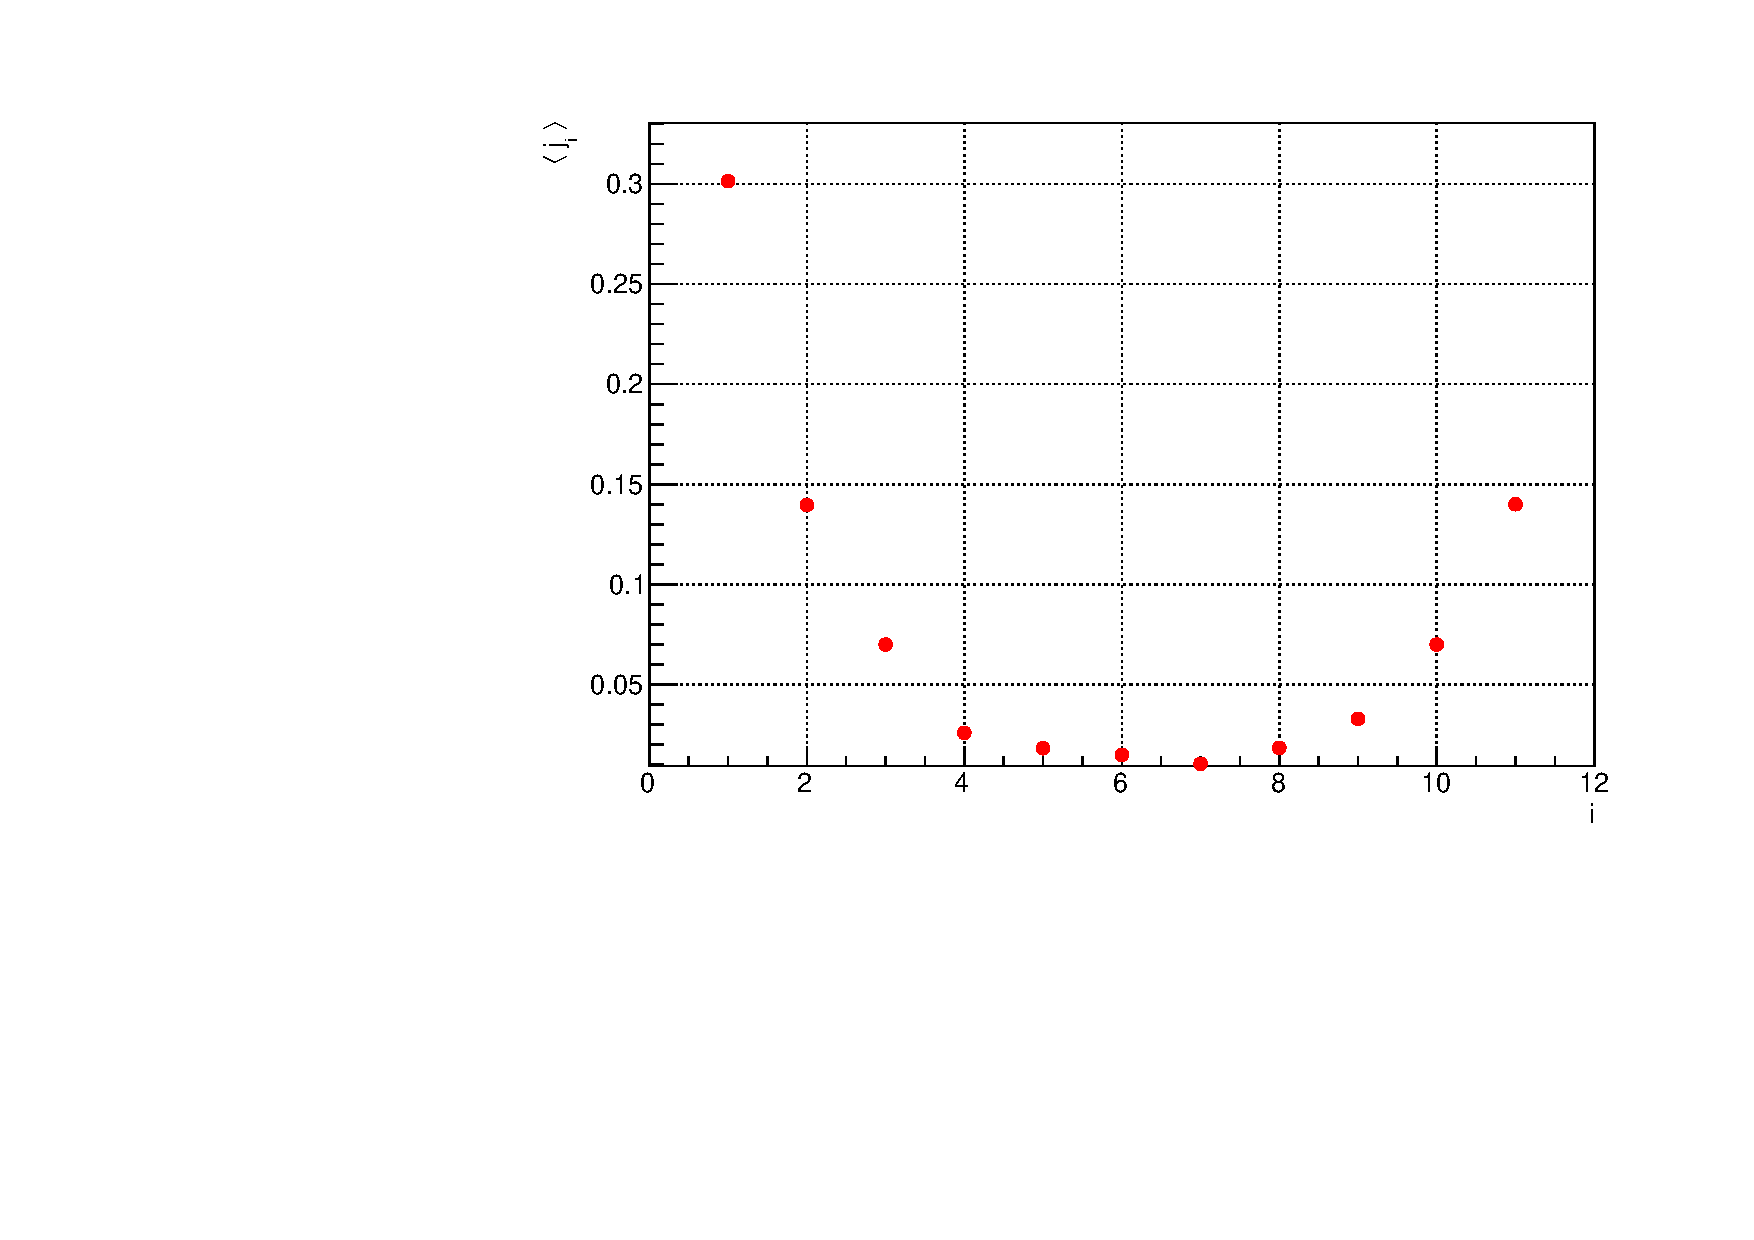
\includegraphics[scale=0.7]{Figures/12sites/SpinCurrL012m060Time002000_J1051.pdf}
%    \caption{Spin current of a 12-sites chain, characterized by $\gamma=1, J_x=1, J_y=0.5, J_z=1.$; %\emph{i} stands for the site index. Data are obtained from MPO method.}
%    \label{fig:my_label}
%\end{figure}
%
%\begin{figure}[H]
%    \centering
%    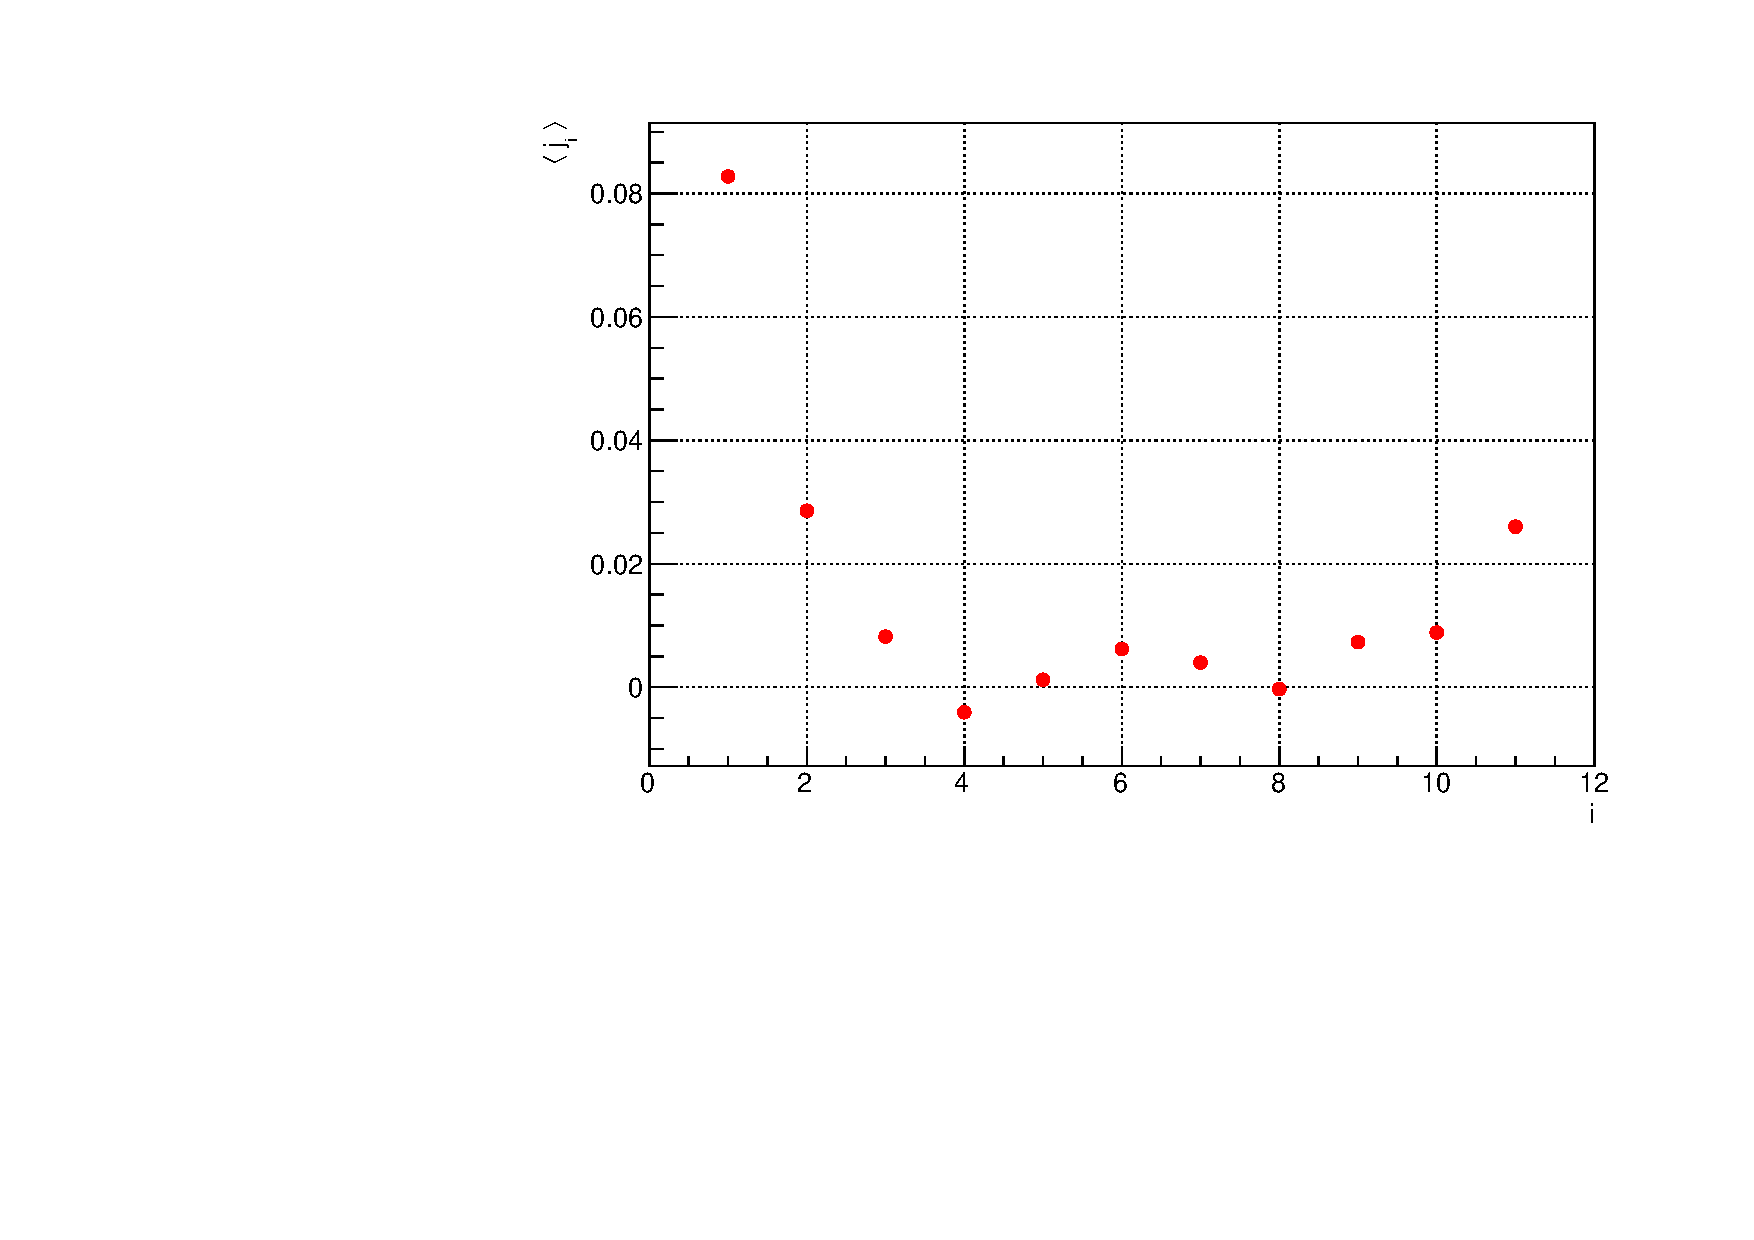
\includegraphics[scale=0.7]{Figures/12sites/SpinCurrL012m060Time002000_J10515.pdf}
%    \caption{Spin current of a 12-sites chain, characterized by $\gamma=1, J_x=1, J_y=0.5, J_z=1.5$; %\emph{i} stands for the site index. Data are obtained from MPO method.}
%    \label{fig:my_label}
%\end{figure}

As done previously for the observables already studied, we can see how the spin current changes for chain of different lengths with the same model. In fig.~\ref{fig:NORM_SpinCurr_comparisonVSsize} it is shown the spin current for a 8, 12 and 16-sites chain, characterized by $J_z = 1$ and dissipation rate $\gamma = 1$. The curves are asymmetric, due to the fact that the Heisenberg model XYZ has an intrinsic anisotropy. While the length of the chain increases, the spin current shows a flatter profile which is consistent with the fig.~\ref{fig:LM_comparisonVSsizeJz1Gamma1} where the plateau of the magnetization becomes bigger while the size of the chain grows.

\begin{figure}[H]
    \centering
    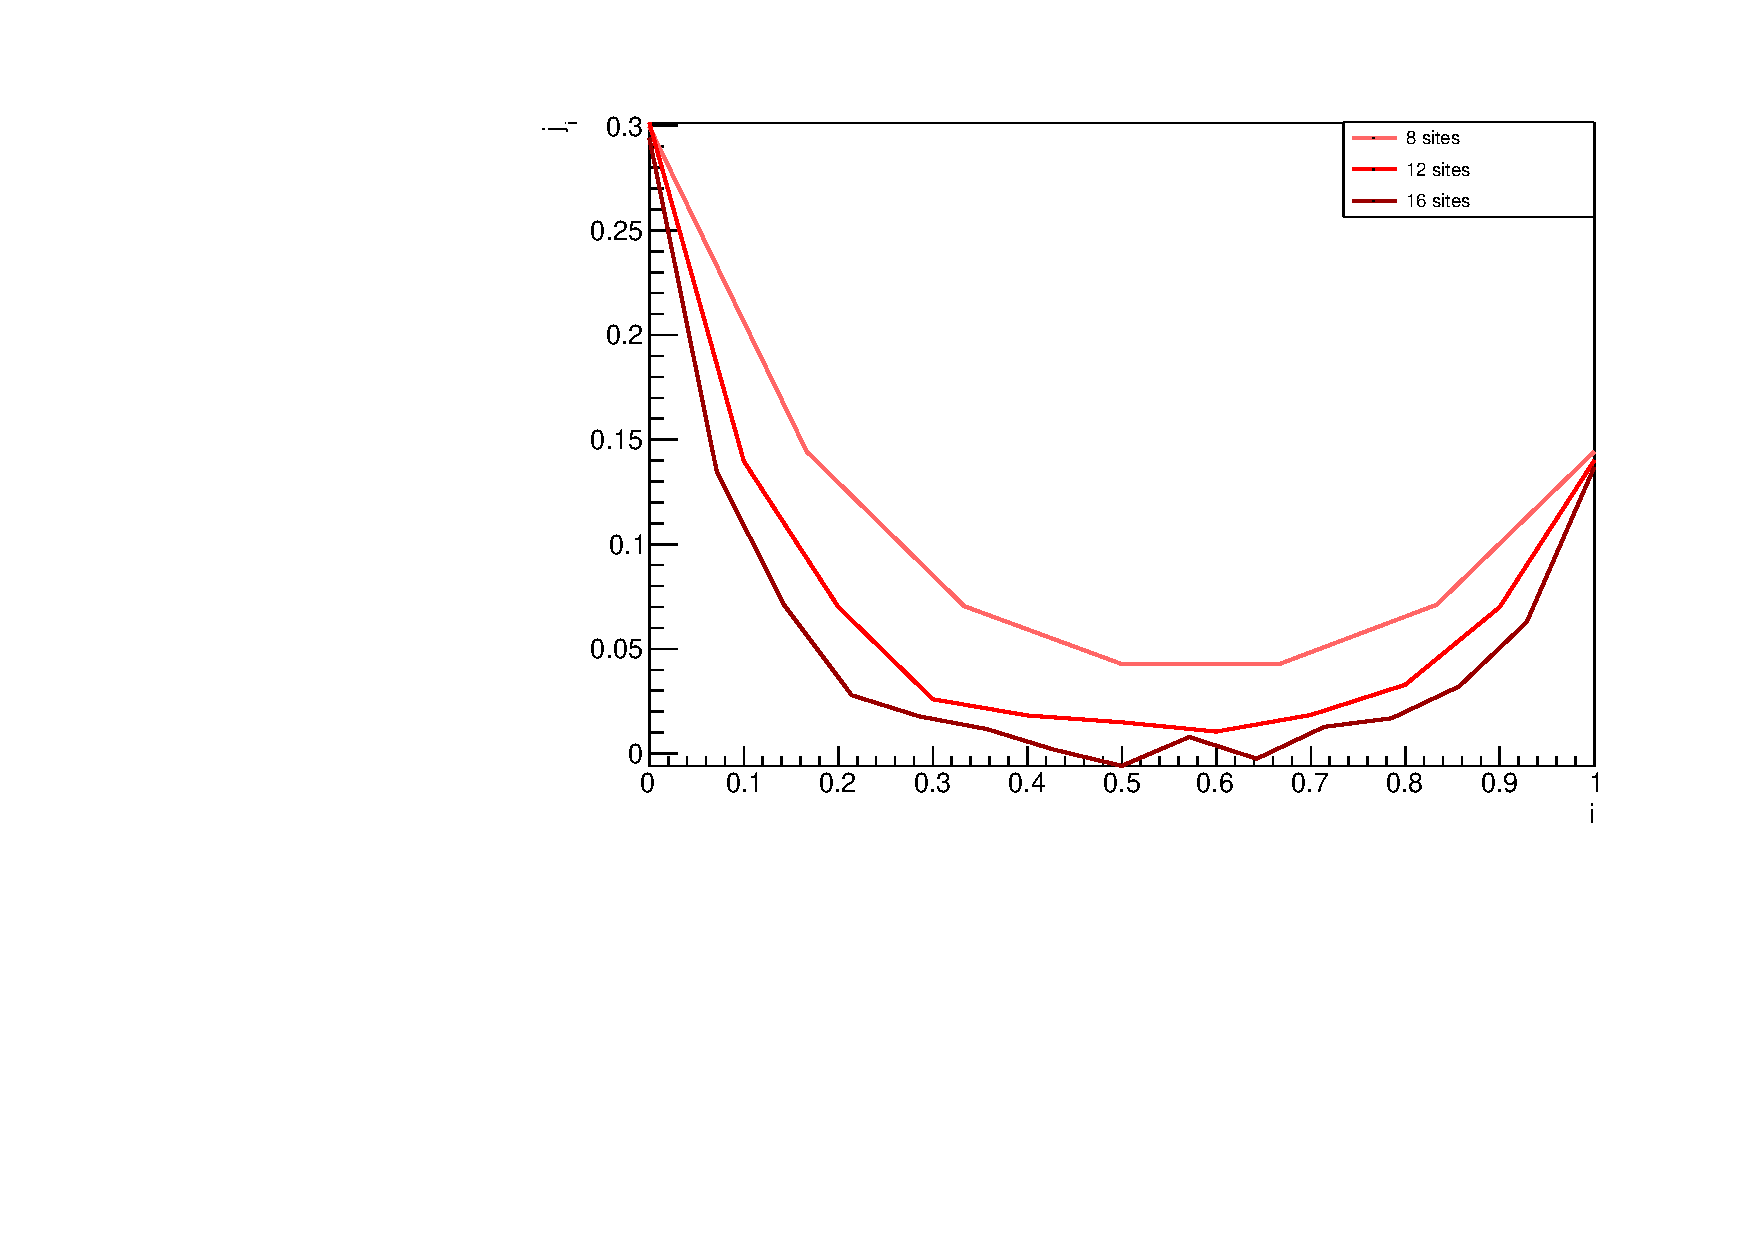
\includegraphics[scale=0.7]{Figures/NORM_SpinCurr_comparisonVSsize.pdf}
    \caption{Spin current for the model at $J_z = 1$. Data for different chain lengths are shown. They are obtained from MPO method. \textcolor{red}{SE RIESCI MODIFICARE PER COLORI}}
    \label{fig:NORM_SpinCurr_comparisonVSsize}
\end{figure}

An aspect worth considering is the common peak value of the spin current, independent of the chain size. As done in the section~\ref{sec:magn_profile} studying the magnetization, we can see how this value changes varying $\gamma$. 

\begin{figure}[H]
    \centering
    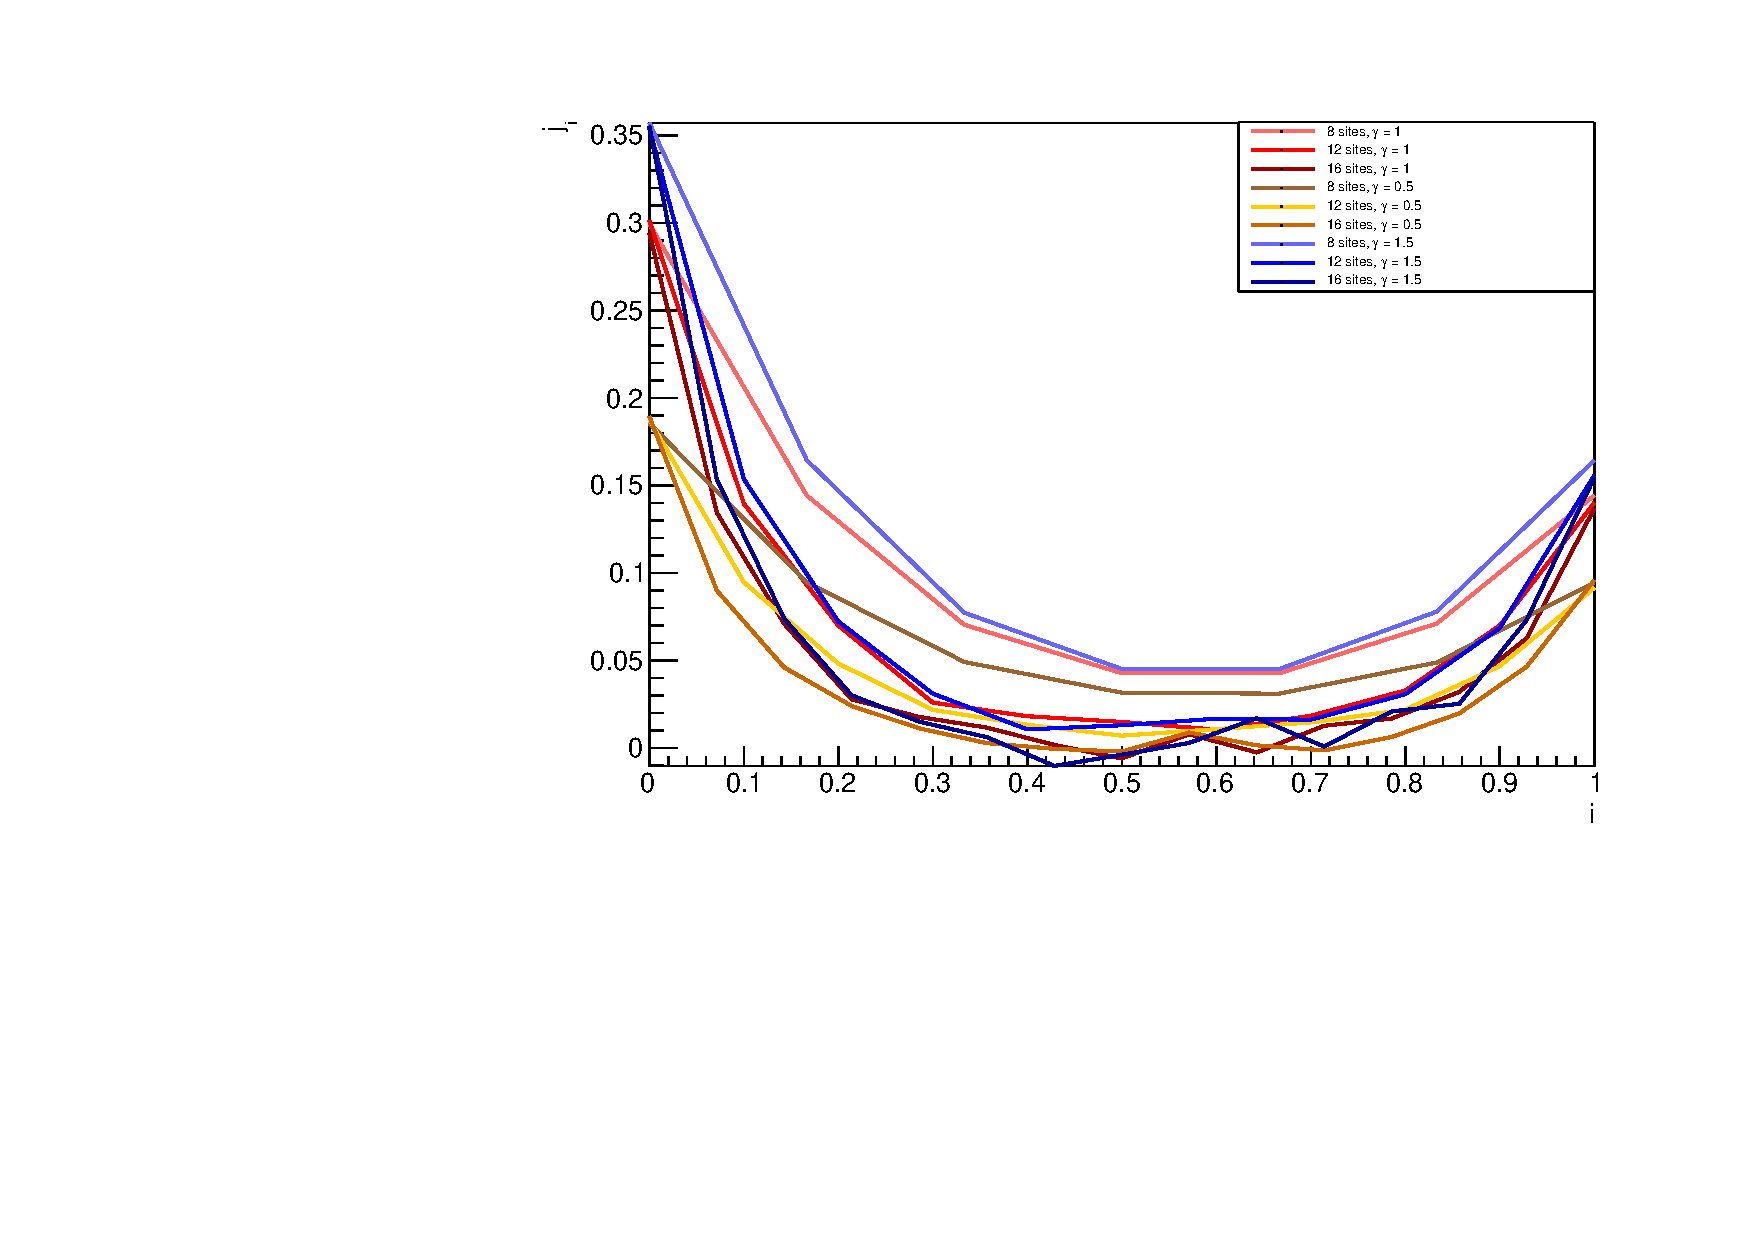
\includegraphics[scale=0.7]{Figures/SpinCurrcomparisonVSsizeANDdissipationRate.pdf}
    \caption{Spin current for the model at fixed $J_z = 1$, for several values of $\gamma$.}
    \label{fig:SpinCurrcomparisonVSsizeANDdissipationRate}
\end{figure}

\begin{figure}[H]
    \centering
    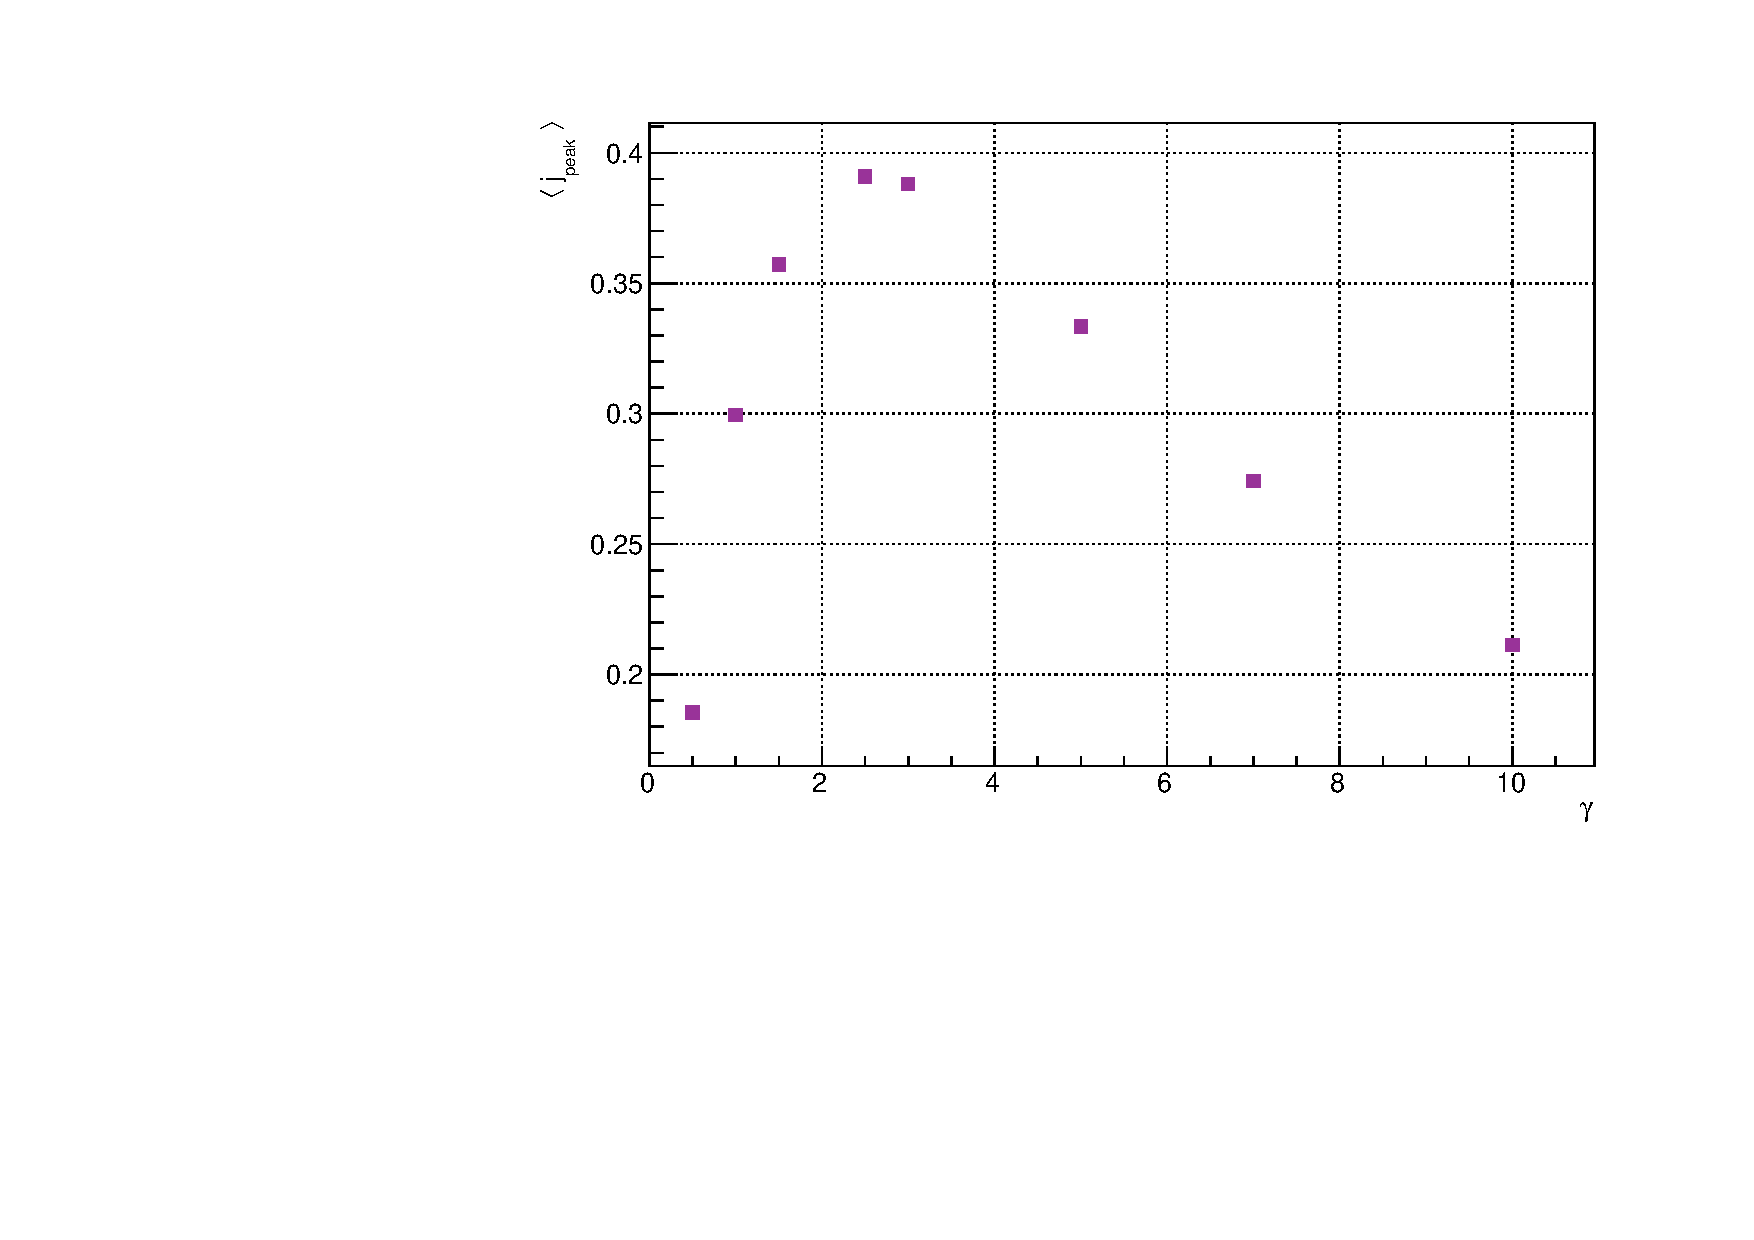
\includegraphics[scale=0.7]{Figures/PeakValueSpinCurrVSgamma_8sites.pdf}
    \caption{Peak values of spin current for several values of $\gamma$. Data are obtained from MPO method.}
    \label{fig:PeakValueSpinCurrVSgamma_8sites}
\end{figure}

%%%%%%%%%%%%%%%%%%%%%%%%%%%%%%%%%%%%%%%%%%%%%%%%%%%%%%%%%%%%%%%%%%%%%%%%%%%%%%%%%%%%%%%%%%%%%%%%%%%%%%%%%%%%%%%%%%%%%%%%%%%%%%%%%%%%%%%%%%%%%%%%%%%%%%%%%%%%%%%%%%%%%%%%%%%%%%%%%%%%%%%%%%%%%%%%%%%%%%
%%%%%%%%%%%%%%%%%%%%%%%%%%%%%%%%%%%%%%%%%%%%%%%%%%%%%%%%%%%%%%%%%%%%%%%%%%%%%%%%%%%%%%%%%%%%%%%%%%%%%%%%%%%%%%%%%%%%%%%%%%%%%%%%%%%%%%%%%%%%%%%%%%%%%%%%%%%%%%%%%%%%%%%%%%%%%%%%%%%%%%%%%%%%%%%%%%%%%%
%%%%%%%%%%%%%%%%%%%%%%%%%%%%%%%%%%%%%%%%%%%%%%%%%%%%%%%%%%%%%%%%%%%%%%%%%%%%%%%%%%%%%%%%%%%%%%%%%%%
\section{Varying J\textsubscript{z}}

Let us have a look to the spin current while varying $J_z$.

\begin{figure}[H]
    \centering
    \includegraphics[scale=0.7]{Figures/8sites_spinCurrVSJz.pdf}
    \caption{8-sites chain.}
    \label{fig:my_label}
\end{figure}


An interesting behaviour is shown for $J_z < 0.5$. Let us go into detail.

\begin{figure}[H]
    \centering
    \includegraphics[scale=0.7]{Figures/8sites_spinCurrVsLOWJz.pdf}
    \caption{8-sites chain.}
    \label{fig:my_label}
\end{figure}

\begin{figure}[H]
    \centering
    \includegraphics[scale=0.7]{Figures/8sites_LMvsJz.pdf}
    \caption{8-sites chain.}
    \label{fig:my_label}
\end{figure}

\begin{figure}[H]
    \centering
    \includegraphics[scale=0.7]{Figures/8sites_LMvsLowJz.pdf}
    \caption{8-sites chain.}
    \label{fig:my_label}
\end{figure}


Let us see if this behaviour still remains in longer chains.

\begin{figure}[H]
    \centering
    \includegraphics[scale=0.7]{Figures/12sites_spinCurrVSJz.pdf}
    \caption{12-sites chain.}
    \label{fig:my_label}
\end{figure}

\begin{figure}[H]
    \centering
    \includegraphics[scale=0.7]{Figures/12sites/12sites_LMvsJz.pdf}
    \caption{12-sites chain.}
    \label{fig:my_label}
\end{figure}

\begin{figure}[H]
    \centering
    \includegraphics[scale=0.7]{Figures/12sites/12sites_LMvsLOWJz.pdf}
    \caption{12-sites chain.}
    \label{fig:my_label}
\end{figure}

\begin{figure}[H]
    \centering
    \includegraphics[scale=0.7]{Figures/16sites/16sites_SpinCurrVsLOWJz.pdf}
    \caption{16-sites chain.}
    \label{fig:my_label}
\end{figure}

\begin{figure}[H]
    \centering
    \includegraphics[scale=0.7]{Figures/16sites/16sites_LMvsLOWJz.pdf}
    \caption{16-sites chain.}
    \label{fig:my_label}
\end{figure}

\textcolor{red}{$J_z > 1.5$}It is interesting how the profile of correlation changes from an exponential behaviour to a linear one. In the following, we will see how this linear profile changes with respect to $\Delta$. The following fits, as all those performed in this thesis, are done by~\cite{root_cern}.
\begin{figure}[H]
    \centering
    \includegraphics[scale=0.7]{Figures/8sites/FIT8sCorrFunc1_MPO_over15.pdf}
    \caption{Data are obtained from QT method.}
    \label{fig:my_label}
\end{figure}